% \documentclass[algorithmlist, figurelist,tablelist, nomlist, master, onside]{config/seuthesiY}
% \documentclass[figurelist,tablelist, nomlist, engineering, openany]{config/seuthesiY}
\documentclass[figurelist,tablelist,nomlist,engineering, openany]{config/seuthesiY}
% \documentclass[ engineering, openany]{config/seuthesiY}
%===============================================================================
% 采用的编译方式为  XELATEX -→  BIBER -→    XELATEX -→    XELATEX
% 为了加快字体的缓存效率 需要在命令行运行 fc-cache
% 对于学位论文需要标注【硕博】
%===============================================================================
\usepackage{multirow}
\usepackage{booktabs}
\usepackage{geometry}
% \geometry{textwidth=14.5cm,top=2.43cm,bottom=3cm,lmargin=3.21cm,
%       rmargin=2.73cm,bindingoffset=0.25in,heightrounded}
% \geometry{lmargin=2.54cm,rmargin=2.54cm}
\usepackage{blindtext}
% %biblatex宏包的参考文献数据源加载方式
\addbibresource[location=local]{config/seuthesiY.bib}
%设置图标序号
\renewcommand {\thetable} {\thechapter{}-\arabic{table}}
\renewcommand {\thefigure} {\thechapter{}-\arabic{figure}}
\usepackage{caption}
\DeclareCaptionLabelSeparator{twospace}{\ ~}   %%这三条语句即可
\captionsetup{labelsep=twospace}

\newtheorem{definition}{Definition}
% \setlength{\baselineskip}{20pt}%固定行距
\linespread{1.25}%修改行距
% \hypersetup{colorlinks=true,linkcolor=black,citecolor=black} %颜色设置
\begin{document}
\begin{sloppypar}
%===============================================================================
%非盲审
% \categorynumber{TP311} % 分类采用《中国图书资料分类法》
% \UDC{004.6}            %《国际十进分类法UDC》的类号
% \secretlevel{公开}    %学位论文密级分为"公开"、"内部"、"秘密"和"机密"四种
% \studentid{184607}   %学号要完整,前面的零不能省略。
% \title{基于知识图谱的IT运维辅助系统设计与实现}{基于知识图谱的 \rotatebox{270}{IT} 运维辅助系统设计与分析}{}{}{Design and Implementation of IT Operation and Maintenance Assistant System Based on Knowledge Graph}{}
% \author{方苏东}{FANG Sudong}
% \advisor{漆桂林}{教授}{QI Guilin}{Prof.}
% \coadvisor{丁岩}{高工}{DING Yan}{Ir.} % 没有% 可以不填
% \degreetype{工程硕士}{Master of Engineering} % 详细学位名称
% \major{软件工程}
% \submajor{软件工程}
% \defenddate{\today}
% \authorizedate{\today}
% \committeechair{}
% \reviewer{}{}
% \department{东南大学软件学院}{SouthEast University}
% 盲审
\categorynumber{TP311} % 分类采用《中国图书资料分类法》
\UDC{004.6}            %《国际十进分类法UDC》的类号
\secretlevel{公开}    %学位论文密级分为"公开"、"内部"、"秘密"和"机密"四种
\studentid{***}   %学号要完整,前面的零不能省略。
\title{基于知识图谱的IT运维辅助系统设计与实现}{基于知识图谱的 \rotatebox{270}{IT} 运维辅助系统设计与分析}{}{}{Design and Implementation of IT Operation and Maintenance Assistant System Based on Knowledge Graph}{}
\author{***}{***}
\advisor{***}{教授}{***}{Prof.}
\coadvisor{***}{高工}{***}{Ir.} % 没有% 可以不填
\degreetype{工程硕士}{Master of Engineering} % 详细学位名称
\major{软件工程}
\submajor{软件工程}
\defenddate{\today}
\authorizedate{\today}
\committeechair{***}
\reviewer{***}{***}
\department{东南大学软件学院}{SouthEast University}



% \seuthesisthanks{本课题的研究来自于与阿里云合作项目}
% \makebigcover

\makecover
\begin{abstract}{故障预测,IT运维,知识图谱,表示学习}
    随着互联网技术的迅猛发展,目前大多数应用软件都建立在一个庞大、繁杂、跨协议层的大型分布式集群中。这类分布式集群的技术、软件、配置通常会不断地演变,难以避免会发生故障。面对海量的监控数据和庞大的系统,IT(Information Technology)运维人员很难做出迅速、准确的运维决策来应对各种故障。近年来,智能运维 (Artificial Intelligence for IT Operations,AIOps)通过引入人工智能技术,提升了IT运维效率。
    % 已有的AIOps方案使用历史数据训练感知机、贝叶斯网、随机森林等机器学习模型,用于异常检测、异常分类、故障预测等以辅助运维,均只停留在算法层面,对知识表示和推理的积累比较少。在AIOps中引入知识图谱能够结构化整合多源异构数据,规范化展示系统运行状态。知识图谱也可以把人对系统的认知、过往的运维经验沉淀成计算机可表示积累的数据,并作为先验知识来辅助运维。另外,知识图谱中经过严格定义的结构化数据使其具备一定的推理与诊断能力,从而辅助IT运维人员进行线上诊断、故障预测等。
    % 停留在算法层面,仅使用历史数据训练机器学习模型,却忽略了历史数据中蕴含的运维知识。这些运维知识,不仅能够解释故障产生过程,还具有通用性能够指导运维。知识图谱可以结构化整合这些历史数据中的知识,进一步辅助线上诊断、故障预测等运维工作。
    
    然而,在实际场景中,IT运维依然面临着三个问题:多源异构数据难以整合、运维知识表示不足和故障难以准确预知。首先,已有的运行状态监测模型都只能整合片面的数据,导致沉淀的运维知识也是片面的。其次,传统的运维知识表示方法局限于知识的显示结构,忽略了运维知识的深层含义。此外,现有的故障预测方法没有引入运维知识,预测结果缺乏可解释性,可靠性低。
    
    基于此,本文提出了有效解决上述问题的IT运维辅助技术,主要包括:    

    (1)提出了自动化构建组件-事件知识图谱的方法,整合了横跨硬件、软件、日志和运行指标的所有数据,使用了机器学习模型生成组件-事件知识图谱,减少了知识图谱构建的人工消耗。

    (2)提出了组件-事件知识图谱的表示学习模型,考虑了实体在不同上下文中含义不同,把实体表示分为了语义表示和结构表示,实现了实体随上下文变化的动态表示,在组件-事件知识图谱三元组分类和链接预测任务上取得了最好的效果。

    (3)提出了引入组件-事件知识图谱的故障预测模型,利用知识图谱识别事件序列中的关键信息,预测出最匹配的故障类型,提高了预测结果的细粒度,增强了可解释性。

    (4)基于上述工作,设计并实现了一个基于知识图谱的IT运维辅助系统。
    
    综上所述,本文利用历史数据自动化构建了知识图谱,提出了针对该类知识图谱的表示学习模型,并将知识图谱引入到了故障预测中,最终设计并实现了一个基于知识图谱的IT运维辅助系统。
    % \begin{itemize}
    %     \item [(1)] 
    %     提出了自动化构建组件-事件知识图谱的方法,设计了6种事件特征,训练了机器学习分类模型判别事件间有无因果关系,进而从历史数据沉淀出了与故障类型对应的组件-事件知识图谱,减少了知识图谱构建的人工消耗。   
    %     \item [(2)]
    %     提出了组件-事件知识图谱的表示学习模型,考虑了相同实体在不同上下文结构中有着不同的含义,实体表示被分为了语义表示和结构表示两部分,实现了实体动态表示。相较于经典的知识图谱表示学习模型,本文模型在组件-事件知识图谱三元组分类和链接预测任务上取得了最好的效果。
    %     \item [(3)]
    %     引入了组件-事件知识图谱进行故障预测,采用了双向记忆网络编码实时事件序列,利用组件-事件知识图谱注意力机制识别重要信息,取得了最佳的故障预测效果。
    %     \item [(4)]
    %     基于上述工作,设计并实现了一个基于知识图谱的IT运维辅助系统。
    %   \end{itemize}

\end{abstract}

% \begin{englishabstract}{Failure Prediction, ITOps, Knowledge Graph, Knowledge Graph Embedding}
%     With the rapid development of internet technology, most applications are built in a large, complicated and distributed cluster across protocol layers. The technology, software and configuration of the distributed cluster are always evolving, and it is difficult to avoid various failures. In the face of massive monitoring data and huge systems, it is difficult for IT Ops(Operations) personnel to make quick and accurate decisions to prevent failures. AIOps (artificial intelligence for it operations) aims to use artificial intelligence technology to improve IT Ops efficiency.
    
%     The existing AIOps programs use historical data to train perceptron, Bayesian, random forest and other machine learning models for anomaly detection,
%     anomaly classification, and failure prediction. It can be seen that AIOps only stays on the algorithm
%     level, and does not use knowledge representation and reasoning. This paper mainly studies IT Ops
%     technology based on knowledge graph, including the following:
%     \begin{itemize}
%         \item [(1)] 
%         The component-event knowledge graph is constructed automatically, and six kinds of event characteristics are designed. The machine learning classification model is trained to judge whether there is causal relationship between event pair, and then the component-event knowledge graph corresponding to fault type is precipitated from historical data, which reduces the labor consumption of knowledge graph construction.
%         \item [(2)]
%         A representation learning model of component-event knowledge graph is proposed. Because exceptions propagate along topology in IT Ops scenarios, and the same entity has different meanings in different context structures, entity representation is divided into semantic representation and structural representation, which realizes dynamic representation of entities with context changes. Compared with the classical knowledge graph representation learning model, the proposed model achieves the best results on the component-event knowledge graph triple classification and link prediction tasks.
        
%         \item [(3)]
%         The component-event knowledge graph is introduced for fault prediction. After the real-time event sequence is encoded by bidirectional memory network, the attention mechanism of knowledge graph is utilized to obtain important information for fault prediction, and the best fault prediction effect is achieved.

%         \item [(4)]
%         Based on the above work, an IT Ops assistant system based on knowledge graph is designed and implemented. 
        
%     \end{itemize}
% \end{englishabstract}

\begin{englishabstract}{Failure Prediction, IT operation and maintenance, Knowledge Graph, Knowledge Graph Embedding}
With the rapid development of internet technology, most applications are built in a large, complicated and distributed cluster across protocol layers. The technology, software and configuration of this kind of distributed cluster are always evolving, and it is difficult to avoid failure. Faced with massive monitoring data and huge systems, it is difficult for IT(Information Technology) operation and maintenance personnel to make quick and accurate operation and maintenance decisions to deal with various failures. In recent years, Artificial Intelligence for IT Operations (AIOps) has improved the efficiency of IT operation and maintenance by introducing artificial intelligence technology. 

However, in the actual scene, IT operation and maintenance still faces three problems: it is difficult to integrate multi-source heterogeneous data, insufficient representation of operation and maintenance knowledge and it is difficult to accurately predict faults. First of all, the existing operational status monitoring models can only integrate one-sided data, which leads to one-sided operation and maintenance knowledge. Secondly, the traditional representation method of operation and maintenance knowledge is limited to the display structure of knowledge, which neglects the deep meaning of operation and maintenance knowledge. In addition, the existing fault prediction methods do not use operation and maintenance knowledge, and the prediction results are lack of interpretability and reliability.

Based on this, this paper proposes an IT operation and maintenance assistant technology to effectively solve the above problems, which mainly includes: 

(1) A method of building component-event knowledge graph automatically is proposed, which integrates all types of data across hardware, software, logs and operation indicators, and uses machine learning model to generate component-event knowledge graph, thus reducing the labor consumption of building knowledge graph.

(2) A representation learning model of component-event knowledge graph is proposed. Considering the different meanings of entity in different contexts, entity representation is divided into semantic representation and structural representation, which realizes the dynamic representation of entity changing with context, and achieves the best results in component-event knowledge graph triple classification and link prediction tasks. 

(3) A fault prediction model based on component-event knowledge graph is proposed. The key information in event sequence is identified by knowledge graph, and the most matching fault type is predicted, which improves the fine granularity of prediction results and enhances the interpretability. 

(4) Based on the above work, an IT operation and maintenance assistant system based on knowledge graph is designed and implemented. 
    
To sum up, this paper uses historical data to build knowledge graph automatically, puts forward a representation learning model for this kind of knowledge graph, introduces knowledge graph into fault prediction, and finally designs and implements an IT operation and maintenance assistant system based on knowledge graph.
\end{englishabstract}
\setnomname{缩略词表}
\tableofcontents
\listofothers
%===============================================================================

% \begin{thenomenclature} 
%     \nomgroup{A}
%         \item [{IT}]\begingroup Information Technology\nomeqref {1.0}\nompageref{6}
%         \item [{Ops}]\begingroup Operations\nomeqref {1.0} \nompageref{6}
%         \item [{AIOps}]\begingroup Artificial Intelligence for IT Operations\nomeqref {1.0}  \nompageref{6}
%         \item [{API}]\begingroup Application Programming Interface\nomeqref {1.0}\nompageref{6}
%         \item [{KPI}]\begingroup Key Performance Indicators\nomeqref {1.0}\nompageref{6}
%         \item [{SLB}]\begingroup Server Load Balancer\nomeqref {1.0} \nompageref{6}
      
%         \item [{ECS}]\begingroup Elastic Compute Service\nomeqref {1.0} \nompageref{6}
%         \item [{RNN}]\begingroup Recurrent Neural Networks\nomeqref {1.0} \nompageref{6}
%         \item [{LSTM}]\begingroup Long Short-Term Memory\nomeqref {1.0} \nompageref{6}
%         \item [{BiLSTM}]\begingroup Bi-directional Long Short-Term Memory\nomeqref {1.0} \nompageref{6}
%         \item [{SVM}]\begingroup Support Vector Machines\nomeqref {1.0} \nompageref{6}
%         \item [{RGCN}]\begingroup Relational Graph Convolutional Networks\nomeqref {1.0} \nompageref{6}
%         \item [{VPC}]\begingroup Virtual Private Cloud\nomeqref {1.0} \nompageref{6}
%         \item [{DTW}]\begingroup Dynamic Time Warping\nomeqref {1.0} \nompageref{6}
%         \item [{k8s}]\begingroup kubeneters\nomeqref {1.0} \nompageref{6}
%         \item [{MR}]\begingroup mean rank\nomeqref {1.0} \nompageref{6}
%         \item [{Hits@n}]\begingroup Hits at n\nomeqref {1.0} \nompageref{6}
%         \item [{HSMM}]\begingroup Hidden Semi-Markov Model\nomeqref {1.0} \nompageref{6}
%         \item [{B/S}]\begingroup Browser/Server\nomeqref {1.0} \nompageref{6}
%         \item [{SLS}]\begingroup Log Service\nomeqref {1.0} \nompageref{6}

% \end{thenomenclature}


% 摘要 版本v1
% 随着互联网、移动互联网的迅猛发展,目前大多数应用软件都建立在一个庞大、复杂、跨协议层的大型分布式系统之上。
% 这个分布式系统的技术、软件、配置通常会不断地演变;其软硬件也难以避免会发生故障和变更;用户流量会发生不可预知的变化,甚至会发生安全攻击事件等等。
% 上述问题都是IT运维(以下简称Ops,包含运维、故障诊断、安全等方面)过程中面临的重要挑战。
% 即使各大集团在运维方面已有大量人力投入,在日常的工作中面对海量的监控数据和庞大的系统,运维人员还是很难做出迅速、准确的运维决策,
% 导致出现各种各样的、甚至影响非常大的故障。

% 近些年被提出的AIOps (Artificial Intelligence for IT Operations)尝试将人工智能的能力与运维相结合,通过机器学习的方法来提升运维效率。已有AIOps方案使用历史数据训练SVM、贝叶斯、随机森林等机器学习模型,用于异常检测、异常分类、根因溯源等辅助运维,仅仅停留在算法层面上,
% 对知识表示和推理的积累比较少。
% 现在业界有大量的静态和动态数据(如设备型号配置信息、设备时序信息、用户软件日志等),
% 整合这些多元异构数据,围绕IT运维构建一套知识库,将会有效服务于集团内的自动化运维。
% 相比于业界主要依赖于算法进行的AIOps,基于运维知识图谱的AIOps能够结构化整合异构复杂数据,
% 对系统实时运行状态进行建模,从而进一步对系统进行自动化检测。
% 另外,知识图谱可以把人对系统的认知、过往的运维诊断经验沉淀成计算机可以表示、积累的数据,
% 并可以在以后的运维过程中,引入这些数据作为先验知识来辅助决策。
% 同时,知识图谱中经过严格定义的结构化数据使其具备一定的推理与诊断能力,从而辅助人进行线上运维、异常排查分析等。

% 本文主要研究在 IT 运维场景中引入知识图谱以辅助运维的技术,主要工作如下:

% (1) 基于机器学习自动化构建组件-事件知识图谱。本文将事件特征拓展至6种,并训练了机器学习分类模型判别事件间有无因果关系,进而利用历史数据沉淀出了组件-事件知识图谱,缓解了知识图谱构建的人工消耗。

% (2) 组件-事件知识图谱表示学习。针对 IT 运维场景下异常沿着拓扑传导的特性,且相同实体在不同上下文环境中有着不同的含义,本文将实体表示分为语义表示和结构表示两部分,实现了实体随着不同上下文变化而动态表示。相较于经典的知识图谱表示模型,本文模型在组件-事件知识图谱三元组分类和链接预测任务上取得了最好的效果。

% (3) 引入知识图谱进行故障预测。本文提出了在双向记忆网络编码事件序列时,引入知识图谱来进行故障预测,取得了最佳的故障预测效果。

% (4) 基于上述工作,设计并实现了一个基于知识图谱的IT运维辅助系统。

\mainmatter

\chapter{绪论}
\section{研究背景与意义}
近年来,由于云计算灵活、便捷、可扩展的特性,越来越多电子商务、社交网络、金融、医药等领域的企业都选择将其服务应用部署于云计算环境中。在云计算环境中,这些服务应用会被部署在复杂庞大、跨协议的分布式集群上。随着分布式集群中的软硬件变迁、技术升级、配置更新等,各种故障时有发生,如资源争用死锁、软件运行错误、硬件故障等。另外,分布式集群结构的复杂性和资源的共享关联性会形成阻力,导致运维人员很难快速准确地查询分析分布式集群数据,进而导致故障未被及时发现而进一步扩散,最终导致应用不可用,带来巨大的经济损失。例如,云提供商AmazonWeb Service(AWS)在2015年9月20日上午2:13到7:10之间发生了一次服务宕机,当时用户无法访问Netflix,Tinder,Airbnb,Reddit和IMDb等流行的在线服务,失败的根源在于美国东部地区亚马逊DynamoDB服务的读写操作异常。

因此,如何借助人工智能技术辅助运维人员自动检测、分析、预测故障成为了研究的热点及难点。近些年被提出的智能运维(AIOps)就尝试将人工智能技术与运维相结合,通过机器学习的方法来提升运维效率。但大量已有AIOps方案均使用历史数据训练各种机器学习模型,用于完成异常检测、异常分类和故障预测等任务,却忽略了历史数据中蕴含的运维知识。这些运维知识,不仅能够解释故障产生过程,还具有通用性能够指导运维。由于缺少对运维知识的研究,AIOps仍然无法解决IT运维所面临的诸多问题。

% 运维知识,对于云服务提供商,可以为客户提供更稳定的服务以增加收益;对于运维人员,可以更直观,更有效地管理分布式集群减少人力消耗,并做出可解释、可靠的运维决策;对于云应用程序开发人员,可以减少应用程序部署,迭代和发布的阻力。
\begin{figure}[htbp]
    \centering
    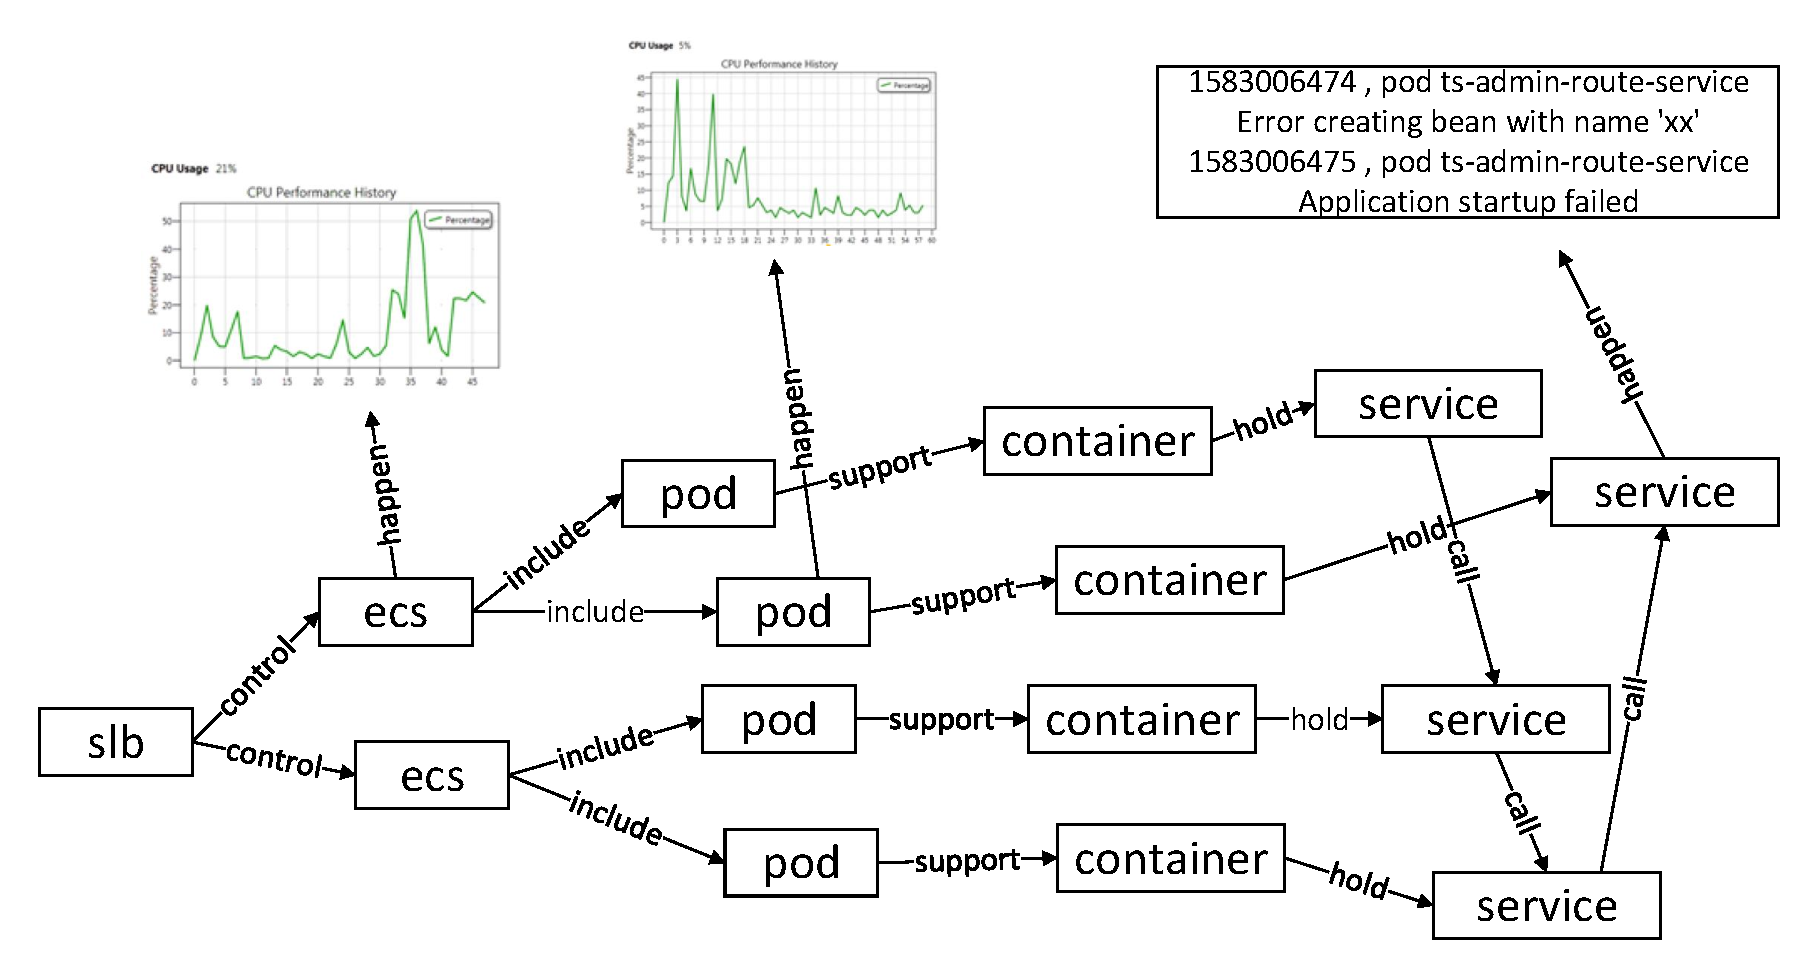
\includegraphics[width=0.9\textwidth]{cloud-environment.pdf}
    \caption{分布式集群信息关系示意图\label{cloud-environment}}
\end{figure}

首先,如何全面地整合多源异构数据,来获取运维知识始终是IT运维面临的一个问题。分布式集群中的数据不仅形式复杂多样,而且数量庞大。如图\ref{cloud-environment}所示,分布式集群中可用的数据包括组件间的拓扑关系、硬件的指标时序数据、软件的运行日志数据。组件间的拓扑关系指明了组件间的交互、依赖等关系,如负载均衡器(Server Load Balancer,SLB)会调控多台云服务器(Elastic Compute Service,ECS)实现负载均衡;硬件的指标时序数据记录了硬件的内存占用率、读写速度、CPU负载率等随时间的变化曲线;软件的运行日志数据记录了各个微服务在具体时间戳打印的日志文本。随着分布式集群的实时运转,平均每秒钟产生的各类数据可达上万条。

已有的运行状态监测模型\cite{wang2019grano,nie2016mining-causality-graph,qiu2020causality-mining-knowledge-graph}可以实时监测、收集分布式集群中的数据,并进一步沉淀运维知识。但其始终无法整合全部数据,都只监测到了片面的数据,导致获取到的运维知识也是片面的。现有运行状态监测模型的覆盖率、细粒度都有待提高,这样才能提升运维知识的全面性和通用性。
% 在已有的研究中,\cite{wang2019grano,nie2016mining-causality-graph,qiu2020causality-mining-knowledge-graph}分别基于系统拓扑图、基于事件因果图、基于运维知识图谱监测集群运行状态,不断收集数据,并从中获取运维知识。但这些方法所监测到的数据都是片面的,导致获取到的运维知识也是片面的。系统拓扑图只关注组件间的交互关系,忽略了异常数据间的触发关系;事件因果图只关注集群异常事件之间的因果关系,忽略了事件所在的组件信息;运维知识图谱只关注数据种类之间的依赖关系,忽略了具体数据间的触发逻辑,构建的知识图谱细粒度较低。可见,现有运行状态监测模型的覆盖率、细粒度都有待提高,这样才能提升运维知识的全面性和通用性。

另外,如何有效地表示运维知识,也是IT运维一个亟待解决的问题。文献\parencite{nie2016mining-causality-graph,qiu2020causality-mining-knowledge-graph,tan2012prepare}将运维知识拓扑视作贝叶斯网,随后利用贝叶斯推理辅助运维工作。但贝叶斯网建立于条件独立性假设上,其认为给定父节点后,每个子节点与其非后代节点条件独立。事实上,在IT运维场景中,条件独立性假设是不成立的,比如故障产生与已发生的多条异常信息、系统整体状态都息息相关。这种运用贝叶斯网建模表示运维知识的方式,对IT运维辅助工作有一定提升,但局限于知识的显示结构,忽略了运维知识的深层逻辑。运维知识的表示,仍具有巨大提升空间。

IT运维还面临着另一个问题是如何准确预知未来可能会出现的故障。故障预测是辅助IT运维的代表性工作,其通过预测可能会发生的故障,提醒运维人员及时采取预防措施。当前,基于深度学习的故障预测方法\cite{xu2016health,cheng2018machine,du2017deeplog,das2018desh,islam2017predicting,li2020predicting,gao2020task}是研究的热点,其可以在故障预测任务上达到很好的预测效果,如文献\parencite{gao2020task}可以达到87\%的准确度和86\%的F1值。但是该类方法只能预测到是否会有故障发生,不能具体到会出现何种故障。另外,由于没引入运维知识,也不能给出故障触发过程,缺乏可解释性,可靠性低。在故障预测中引入运维知识,提高预测结果细粒度,增强预测可解释性,是目前亟待展开的工作。

% 基于以上分析,首先本文分析了现有的分布式集群运行状态监测方案,发现这些方案仅使用了分布式集群部分信息且挖掘的数据特征有限,导致构建的监测拓扑图比较片面且其构建过程需要大量人工。本文收集了横跨软硬件的所有信息,并设计了6种数据特征,构建了组件-事件知识图谱。其次,本文针对云计算场景下异常沿组件图传播、事件发生与上下文相关的特性,提出了组件-事件知识图谱实体的动态表示方案。最后,本文用双向记忆网络编码事件序列,再用组件-事件知识图谱识别关键信息,从而将运维知识引入到故障预测中,增强了预测结果的可靠性与可解释性。
综上所述,目前在IT运维领域存在着以下挑战:
% \begin{itemize}[itemsep=0pt,parsep=0pt]
%     \item [(1)]在沉淀运维知识时,存在多源异构数据难以整合的挑战,已有的运行状态监测模型从不同方面获取集群运行状态信息,但都具有片面性,存在着巨大的提升空间。
%     \item [(2)]在表示运维知识时,存在运维知识表示不足的挑战,基于贝叶斯网建模表示的方式局限于显示的知识拓扑结构,需要进一步展开针对运维知识的表示学习研究。
%     \item [(3)]在故障预测时,存在着故障难以准确预知的挑战,只依靠深度学习的故障预测方法预测结果细粒度低,缺乏可解释性,需要展开引入运维知识进行故障预测的研究。
%     \item [(4)]针对上述的挑战,需要实现一种满足运维人员需求的IT运维辅助系统。该系统需要能够监测多源异构数据,有效地沉淀、表示运维知识,并用于实时的故障预测。
% \end{itemize}

(1)在沉淀运维知识时,存在多源异构数据难以整合的挑战,已有的运行状态监测模型从不同方面获取集群运行状态信息,但都具有片面性,存在着巨大的提升空间。

(2)在表示运维知识时,存在运维知识表示不足的挑战,基于贝叶斯网建模表示的方式局限于显示的知识拓扑结构,需要进一步展开针对运维知识的表示学习研究。

(3)在故障预测时,存在着故障难以准确预知的挑战,只依靠深度学习的故障预测方法预测结果细粒度低,缺乏可解释性,需要展开引入运维知识进行故障预测的研究。

(4)针对上述的挑战,需要实现一种满足运维人员需求的IT运维辅助系统。该系统需要能够监测多源异构数据,有效地沉淀、表示运维知识,并用于实时的故障预测。

基于以上背景信息,本文收集了横跨软硬件的所有信息,构建了组件-事件知识图谱。其次,本文提出了组件-事件知识图谱实体的动态表示方案。随后,本文用双向记忆网络编码事件序列,再用组件-事件知识图谱识别关键信息,进行故障预测。最后,本文设计并实现了一个基于知识图谱的IT运维辅助系统。

\section{国内外研究现状}
为了解决IT运维实际中面临的问题,包括多源异构数据难以整合、运维知识表示不足和故障难以准确预知,国内外已经展开了大量研究。本文主要从分布式集群运行状态监测模型、知识表示学习和故障预测三方面展开了调研,并进行了分析。
\subsection{运行状态监测模型研究现状}
有效的分布式集群运行状态监测模型可以全面完善地获取、表示系统运行状态。高细粒度的运行状态数据是展开进一步运维工作的基础。

已有的模型分为基于系统拓扑图的方法、基于事件因果图的方法和基于运维知识图谱的方法。在基于系统拓扑图的方法中,eBay提出的GRANO\cite{wang2019grano}通过构建组件拓扑图,捕获警报信息和程序运行状态,实现了用于云计算分布式数据平台的端到端状态检测分析系统。具体实现上,GRANO首先处理大量指标时序数据来检测硬件和软件系统组件的异常信息,随后让专家利用领域知识给异常信息打上严重分数,然后在组件拓扑图上使用传播算法对各个组件的严重分数进行更新,最终辅助运维人员通过交互界面沿着系统拓扑图查看严重的系统组件。这种基于系统拓扑图的方法虽可以有效监视和识别系统异常,但不能沉淀出运维知识,也不能给出可靠的异常触发链。在基于事件因果图的方法中,文献\parencite{nie2016mining-causality-graph}首先利用异常检测方法\cite{nguyen2011pal}获取各个系统组件实时运行发生的异常事件,随后借助有监督的机器学习\cite{breiman2001randomforest}构建事件间可靠的因果关系,最终形成可辅助运维的事件因果图。这种基于事件因果图的方法不需要了解云计算场景中应用的设计和实现细节,也不需要检测服务的源代码,但只使用概率特征的因果发掘模型需要领域专家循环标注海量数据才可以达到良好的效果,且缺乏对系统组件拓扑关系的有效利用。在基于运维知识图谱的方法中,文献\parencite{qiu2020causality-mining-knowledge-graph}根据组件间的访问与部署关系、指标与组件间的来源产生关系,构建了运维知识图谱,但对于异常信息间的触发关系,该图谱只能精确到指标时序类型之间的因果关系,如“Container 1 CPU usage”导致了“Microservice 1 Response Time”\cite{qiu2020causality-mining-knowledge-graph},不能进一步知道什么样的CPU变化导致了什么样的响应时间变化。

可见始终缺乏一个横跨硬件、软件、异常数据,并能在高细粒度上将异常信息触发链和系统状态作为知识沉淀下来的运行状态监测模型。
\subsection{知识表示学习研究现状}\label{kge-research}
在运行状态监测模型沉淀出知识后,需要利用知识表示学习将运维知识转为计算机可理解的数据形式,即利用计算机可以处理的实值向量来表示知识实体和关系。运维知识被转化为实值向量后,可以通过计算机引入到下游任务中(如故障预测),有助于实现自动化运维。

知识表示学习方面,已经存在着大量工作。基于距离的模型中,文献\parencite{bordes2012joint}只利用了头实体和尾实体的共现信息来进行表示学习;在此基础上文献\parencite{bordes2011learning}将实体关系建模为两个分别针对头尾实体的矩阵,从而引入了关系信息。从翻译视角展开工作的模型中,最开始TranE\cite{bordes2013translatingE}将每个知识三元组中的关系视作头实体到尾实体的翻译过程,但它不能处理复杂的一对多、多对多关系;TransH\cite{wang2014knowledge}选择将头尾实体都映射到关系所在的超平面上,解决了复杂关系的问题;TransR\cite{lin2015learning}认为每一种关系间是有区别的,应该对应着不同的语义向量空间,所以其将关系嵌入为矩阵;TransD\cite{ji2015knowledge}为了克服同一关系头尾实体种类属性差别过大的问题,将每个对象(实体、关系)嵌入为语义向量和映射向量这两个向量;TranSparse\cite{ji2016knowledge}根据关系连接的头尾实体对数量,自适应的调整映射矩阵的稀疏程度;TransF\cite{feng2016knowledge}放宽了损失函数的约束条件,只要求头实体加关系后的张量与尾实体关系一致;TransG\cite{ou2016asymmetric}将实体的不确定度、关系的多语义用高斯分布协方差来表示。基于语义匹配的模型中,LFM\cite{jenatton2012latent}使用关系的双线性变换,刻画实体和关系之间的二阶联系;ComplEx\cite{trouillon2016complex}为了建模非对称关系将表示扩展到复数向量空间;ANALOGY\cite{liu2017analogical}将知识图谱中的类比关系进行了建模;SLM\cite{socher2013reasoning}开始引入神经网络,其利用标准非线性单层神经网络来连接实体;NTN\cite{socher2013reasoning}使用张量网络捕获头尾实体间的语义关联;ConvE\cite{dettmers2018convolutional}为了捕获实体间的语义关系,使用了卷积网络。融入多源信息的模型也有很多,SSE\cite{guo2015semantically}和TKRL\cite{xie2016representation}将实体的类别信息引入了知识表示学习中;文献\parencite{lin2015modeling}为了引入关系路径将路径上所有的关系向量进行了组合以表示路径向量;为了引入文本描述,文献\parencite{socher2013reasoning}将语料库训练的词向量累加平均作为实体的初始向量;文献\parencite{xie2016representation}给每个实体赋予了基于结构和基于文本描述的两个表示;文献\parencite{wang2016text}选择将实体与文本库词汇对齐;GAKE\cite{feng2016gake}和TCE\cite{shi2017knowledge}则引入了实体的上下文信息,包括邻居上下文、边上下文、路径上下文等。文献\parencite{schlichtkrull2018modeling}引入图卷积网络的同时区分了不同关系对节点的影响,利用图信息传播机制编码知识图谱以获取实体表示。

虽然知识表示学习方面已经存在了很多不同角度展开的工作,但都只能得到实体、关系的静态表示向量。在云计算场景下的组件-事件知识图谱中,实体会随着上下文场景变化有不同的含义,需要动态地表示。
\subsection{故障预测研究现状}
故障预测是一种主动预防故障的方法,可以在故障发生前进行预测,从而告知运维人员采取措施防止故障发生,避免故障造成的损失。
% 马尔科夫模型是一种广泛应用于时间序列数据建模的统计方法。作为有限时间马尔可夫链(DTMC)的扩展,隐马尔可夫模型(HMM)已经成功地应用于许多模式识别任务中,比如语音处理和基因序列分析。尽管基于隐马尔可夫模型的异常预测是近年来众多研究的主题,但要其满足商业应用需求(例如,高可扩展性和预测精度)仍然是一个挑战。

文献\parencite{salfner2010survey}已经对在线故障预测技术进行了广泛地调研。其将现有的故障预测方法宽泛地分为两类:分类方法和函数逼近方法。基于分类的故障预测方法\cite{tan2012prepare,pitakrat2018hora,zhang2018prefix,baldoni2015line}首先构建了容易发生故障和不容易发生故障的数据样本,随后在这些数据上训练分类器。分类器的决策边界通常来自于参考数据集,这个数据集每个数据点的决策边界都是已知的,即明确地知道它指示的是容易发生故障还是不容易发生故障。在进行在线故障预测时,只需要检查当前监视值位于决策边界的哪一侧即可。函数逼近是一个广泛应用于各种科学领域的术语,可以用在故障预测任务的原因在于该任务可以被视作发掘一种函数映射关系,即被监视的系统状态(函数的输入)到系统未来是否会有故障(函数的输出)之间的未知函数关系。逻辑回归技术就是为目标性能值建立曲线拟合函数,并调整参数以最佳拟合训练数据集,其输入数据一般是性能指标时序数据\cite{salfner2010survey}。文献\parencite{dalmazo2013predicting}提出了一种基于统计模型的流量预测方法,它将滑动窗口内的观测值用泊松分布加权。文献\parencite{sladescu2012event}提出了一种事件感知策略,通过利用与计划事件相关的先验知识,可以更有效地预测系统工作时的负载突发。事件感知预测方法可以非常有效地预测故障,但无法给出故障出现的触发过程。文献\parencite{purushotham2005multi}使用了基于隐马尔可夫模型的方法来推断受监控组件的状态是否健康。虽然作者文中未提及该方法可用于故障预测,但可以通过以下方式进行故障预测:假设系统中存在导致未来故障的错误状态,而其他错误状态不会导致未来的故障,所提出的隐马尔可夫模型方法就可以用来确定(分类)故障是否即将发生。文献\parencite{boutros2011detection}指出,可以通过识别系统正在经历的状态来预测系统出现故障的概率,但作者并没有给出详细的算法和实验结果。文献\parencite{xu2016health,cheng2018machine,du2017deeplog,das2018desh,islam2017predicting,li2020predicting}开始使用深度学习方法,如循环神经网络(Recurrent Neural Networks,RNN)和长短期记忆神经网络(Long Short-Term Memory,LSTM)进行故障预测。文献\parencite{gao2020task}使用双向的长短期记忆神经网络(Bi-directional Long Short-Term Memory,BiLSTM)编码时序信息,并对数据赋予了不同权重,在预测是否会发生故障时取得了最佳效果。

从以上调研结果可见,目前的故障预测工作专注于预测是否会有故障发生,不能预测到具体会有何种故障。另外,由于预测过程均没有引入运维知识,预测结果的可解释性不高。
\section{论文研究目标与内容}
\subsection{研究目标}
本文的研究目标是设计并实现一个满足实际运维需求的IT运维辅助系统。为了达到研究目标,本文分析了目前的研究难点,并逐一展开了调研,总结了现有工作存在的问题。在此基础上,本文提出了一个基于知识图谱的IT运维辅助系统的设计方案。该方案基于本文提出的算法模型,将知识图谱构建、知识图谱表示学习、故障预测封装为多个功能模块,以应对多源异构数据难以整合、运维知识表示不足和故障难以准确预知等问题。

\subsection{研究内容}
本文主要开展了以下研究工作:
% \begin{itemize}
%     \item [(1)]研究横跨硬件、软件、异常数据的组件-事件知识图谱自动构建方案。一方面研究如何让知识图谱整合高细粒度的多种信息,如软硬组件间关系、指标时序数据、日志数据。另一方面研究如何设计事件特征,使用机器学习模型挖掘事件间因果关系。最终实现从历史数据中沉淀出故障类型对应的组件-事件知识图谱。
%     \item [(2)]研究针对组件-事件知识图谱的知识表示学习模型。在组件-事件知识图谱中,异常会沿着组件拓扑关系传递,事件间有因果触发关系,实体在不同的上下文中也有不同的含义。针对组件-事件知识图谱的这些特性,需要重点研究如何让实体随上下文变化动态地表示。
%     \item [(3)]研究基于组件-事件知识图谱的故障预测模型。为了解决深度学习模型在故障预测时,可解释性低、预测结果细粒度低的问题,需要研究如何结合知识图谱与深度学习模型进行故障预测。最终使得预测结果可以具体到会出现何种故障,并能结合知识图谱得到触发逻辑。
%     \item [(4)]研究基于知识图谱的IT运维辅助系统的设计与实现。为了满足运维人员使用需求,需要研究如何整合业务流程。重点研究如何实现分布式集群不同信息的实时快速获取,以及如何向运维人员展示运行状态信息和故障预测结果。
% \end{itemize}

(1)研究横跨硬件、软件、异常数据的组件-事件知识图谱自动构建方案。一方面研究如何让知识图谱整合高细粒度的多种信息,如软硬组件间关系、指标时序数据、日志数据。另一方面研究如何设计事件特征,使用机器学习模型挖掘事件间因果关系。最终实现从历史数据中沉淀出故障类型对应的组件-事件知识图谱。

(2)研究针对组件-事件知识图谱的知识表示学习模型。在组件-事件知识图谱中,异常会沿着组件拓扑关系传递,事件间有因果触发关系,实体在不同的上下文中也有不同的含义。针对组件-事件知识图谱的这些特性,需要重点研究如何让实体随上下文变化动态地表示。

(3)研究引入组件-事件知识图谱的故障预测模型。为了解决深度学习模型在故障预测时,可解释性低、预测结果细粒度低的问题,需要研究如何结合知识图谱与实时数据进行故障预测。最终使得预测结果可以具体到会出现何种故障,并能结合知识图谱得到触发逻辑。

(4)研究基于知识图谱的IT运维辅助系统的设计与实现。为了满足运维人员使用需求,需要研究如何整合业务流程。重点研究如何实现分布式集群不同信息的实时快速获取,以及如何向运维人员展示运行状态信息和故障预测结果。

\section{论文结构安排}
本文篇幅结构共有七章,各个章节间的关系如图\ref{paper-constructure}所示,每一章内容如下:

第一章为绪论,首先梳理了相关研究背景和研究现状,然后分点描述了本文研究内容。

第二章为相关技术,描述了本文会涉及到的相关概念及技术,为下文各个方法模型的提出做好铺垫。

第三章为组件-事件知识图谱的构建流程,主要介绍了系统运行状态信息获取,事件因果关系挖掘和历史数据沉淀生成组件-事件知识图谱的过程,在模拟构建的数据集上进行了实验,并分析了实验结果。

第四章为组件-事件知识图谱的知识表示学习,主要分析了场景特性,介绍了随上下文变化的动态表示学习方案,在三元组分类和链接预测任务上进行了对比实验,并分析了实验结果。

第五章为引入组件-事件知识图谱的故障预测,主要介绍了引入组件-事件知识图谱,结合实时事件序列做出可解释故障预测的方法,在事件序列故障预测任务上进行了对比实验,并分析了实验结果。

第六章为系统设计与实现,主要介绍基于本文方法实现了一个基于知识图谱的IT运维辅助系统,并详细介绍该系统的设计和实现细节。

第七章为总结与展望,对本文完成的工作进行了总结归纳,也对未来的工作进行了规划。
\begin{figure}[htbp]
    \centering
    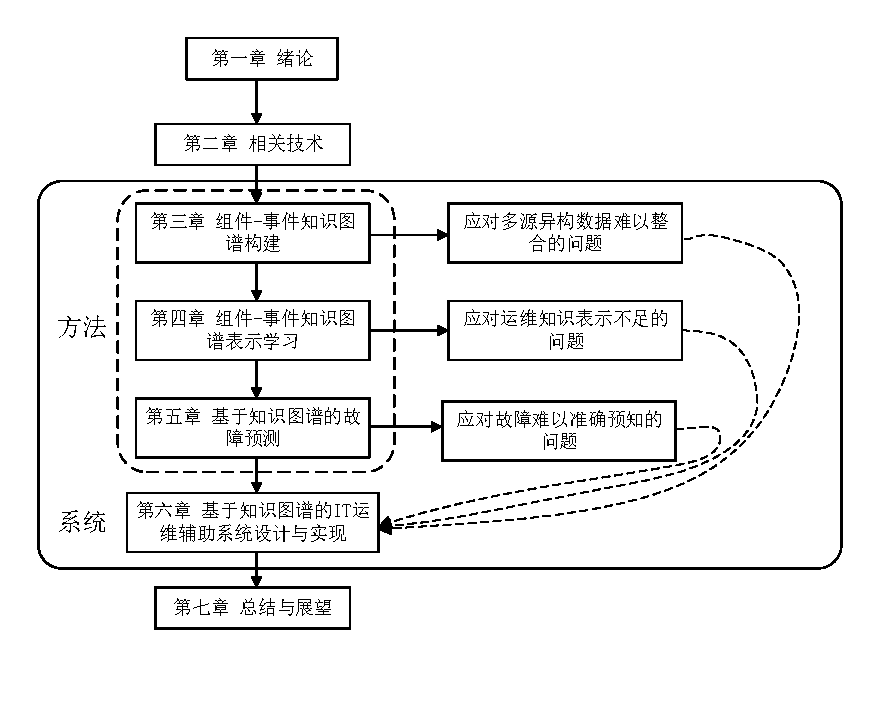
\includegraphics[width=.9\textwidth]{paper-constructure.pdf}
    \caption{论文章节关系示意图\label{paper-constructure}}
\end{figure}

% Definition of rule: E is symptom events unit, A; B 2
% E; A ! B means A causes B and A happens before B. !
% presents the causality.


% 详见文献\parencite{Peebles2001-100-100}\cite{Babu2014--}
% 参考文献\parencite[见][49页]{于潇2012-1518-1523}\cite[见][49页]{Babu2014--}
% 硕士论文\cite{zhouGPS2015},博士论文\cite{余勇1998--}
% 大小写\cite{liu_statistical_2017}

\nomenclature{IT}{Information Technology}
\nomenclature{Ops}{Operations}
\nomenclature{KPI}{Key Performance Indicators}
\nomenclature{AIOps}{Artificial Intelligence for IT Operations}
\nomenclature{API}{Application Programming Interface}

% 如图\ref{lxfbook}所示。

% \begin{figure}
%     \centering
%     \includegraphics[width=.6\textwidth]{lxfbook.jpg}
%     \caption{陆小凤传奇\label{lxfbook}}
% \end{figure}

\chapter{背景知识}
本章主要对本文所涉及的支持向量机、关系图卷积神经网络、双向长短期记忆神经网络、注意力机制等展开了详细的描述,为下文第三章、第四章和第五章的内容做好铺垫。

在构建组件-事件知识图谱时,第三章通过实验分析最终选用了支持向量机发掘事件因果关系,因此本章第一节对支持向量机进行了介绍。第四章组件-事件知识图谱表示学习是基于关系图卷积神经网络提出的,为了便于理解这部分内容,本章第二节对关系图卷积神经网络进行了必要地介绍。第五章基于知识图谱的故障预测是基于双向长短期记忆网络提出的,所以本章第三节对双向长短期记忆网络展开介绍。另外,第四章和第五章所提出的方法,都引入了注意力机制,所以本章第四节又介绍了注意力机制。

\section{支持向量机}
支持向量机(Support Vector Machines,SVM)是机器学习和模式分类领域的经典模型\cite{cherkassky2004practical},通过在输入空间中实现线性或非线性分离面来实现分类。在支持向量分类中,分离函数可以表示为与支持向量相关的核的线性组合,如式\ref{bk-svm}所示:
\begin{equation}
    \centering
    f(x)=\sum_{x_{j} \in S} \alpha_{j} y_{j} K\left(x_{j}, x\right)+b
    \label{bk-svm}
\end{equation}
其中$x_{i}$表示训练模式,$y_{i} \in\{+1,-1\}$表示相应的类标签,$S$表示支持向量集\cite{cherkassky2004practical}。其对偶式如式子\ref{bk-svm-op}所示:
\begin{equation}
    \centering
    \min _{0 \leq \alpha_{i} \leq C} W=\frac{1}{2} \sum_{i, j} \alpha_{i} Q_{i j} \alpha_{j}-\sum_{i} \alpha_{i}+b \sum_{i} y_{i} \alpha_{i}
    \label{bk-svm-op}
\end{equation}
其中$\alpha_{i}$是相应的协同系数,$b$是偏移系数,$Q_{i j}=y_{i} y_{j} K\left(x_{i}, x_{j}\right)$是一个对称的正定核矩阵,$C$是在不可分的情况下用来惩罚误差点的参数\cite{cherkassky2004practical}。对偶的Karush-Kuhn-Tucker(KKT)条件如式\ref{bk-svm-KKT}和式\ref{bk-svm-KKT-2}所示:
\begin{equation}
    \centering
    g_{i}=\frac{\partial W}{\partial \alpha_{i}}=\sum_{i} Q_{i j} \alpha_{j}+y_{i} b-1=y_{i} f\left(x_{i}\right)-1
    \label{bk-svm-KKT}
\end{equation}
\begin{equation}
    \centering
    \frac{\partial W}{\partial b}=\sum_{j} y_{j} \alpha_{j}=0
    \label{bk-svm-KKT-2}
\end{equation}

其将训练集划分为支持向量集$S$$\left(0<\alpha_{i}<C, g_{i}=0\right)$,误差集$E$$\left(\alpha_{i}=C, g_{i}<0\right)$和分类集$R$$\left(\alpha_{i}=0, g_{i}>0\right)$\cite{cauwenberghs2001incremental}。如果误差点用惩罚因子$C^{\prime}$进行二次罚分,那么这表明问题已经被简化为$C=\infty$的可分情形\cite{frie1998kernel}。内核函数可以修改为式\ref{bk-svm-modekernel}所示。
\begin{equation}
    \centering
    K^{\prime}\left(x_{i}, x_{j}\right)=K\left(x_{i}, x_{j}\right)+\frac{1}{C^{\prime}} \delta_{i j}
    \label{bk-svm-modekernel}
\end{equation}

其中当$i=j$时$\delta_{i j}=1$,否则$\delta_{i j}=0$。这个公式的优点是SVM问题可以被简化为线性可分情形\cite{keerthi2000fast}。

由上可见,训练SVM时要解一个二次优化问题,这需要使用来自数值库的优化例程。另外,解二次优化问题是计算密集型的,可能会遇到稳定性问题,并且实现起来非常困难\cite{zeng2008fast}。因此,序列最小优化(Sequential Minimal Optimization,SMO)\cite{keerthi2000fast}和最近点算法(NearestPoint Algorithm ,NPA)\cite{zeng2008fast},相继被提出并成功克服了这个问题。


\section{关系图卷积神经网络}\label{RGCN}
本小节主要介绍关系图卷积神经网络(Relational Graph Convolutional Networks,RGCN)算法\cite{schlichtkrull2018modeling}。该算法区分了不同关系对节点的影响,利用图信息传播机制获取了实体的上下文信息。本节会进一步分为两小节分别介绍RGCN的模型结构和优化目标。
% 下一小节中,本文在此模型基础上考虑了图信息传播时同一关系下不同实体的权重。
\subsection{模型结构}
本小节介绍RGCN的模型结构,包括嵌入层和图卷积层。

嵌入层主要为了引入实体多维度的信息,如实体包含着的各种语义信息。对于每个实体,该文献将其不同的文本属性连接起来,并使用预先训练的Bert\cite{devlin2018bert}模型来获得它们的嵌入表示。这些嵌入表示形成了实体的初始特征向量。对于实体没有属性的数据集,嵌入层则是随机初始化的。

图卷积层使用图卷积网络将局部的信息通过关系传递到整个图中,因此可以将其理解为一个可微分的消息传递框架,可以用式子\ref{propo-example}表示。
\begin{equation}
    h_{i}^{(l+1)}=\sigma\left(\sum_{m \in \mathcal{M}_{i}} g_{m}\left(h_{i}^{(l)}, h_{j}^{(l)}\right)\right)
    \label{propo-example}
\end{equation}

$h_{i}^{(l)} \in \mathbb{R}^{d^{(l)}}$是结点$v_{i}$在$l$-th层神经网络的隐状态,$d^{(l)}$是该层隐状态向量的维度。$g_{m}(\cdot, \cdot)$函数计算了$v_{j}$传入结点$v_{i}$的信息。随后累加$v_{i}$每个邻居结点传来的信息,并将累计结果传入激活函数$\sigma(\cdot)$就可以得到$v_{i}$在下一层神经网络的隐状态向量$h_{i}^{(l+1)}$,其中激活函数可以使用$\operatorname{ReLU}(\cdot)=\max (0, \cdot)$等常见的激活函数。$\mathcal{M}_{i}$表示每一条传入结点$v_{i}$的信息汇总集,其中每一条传入信息都与一条边对应。$g_{m}(\cdot, \cdot)$通常为信息计算函数,具体实现上可以是某种神经网络也可以是某种线性转变,比如$g_{m}\left(h_{i}, h_{j}\right)=W h_{j}$,$W$为参数张量(如文献\parencite{kipf2016semi}所示)。这样的信息计算函数有效地累计并编码了来自局部的结构化邻域特征,并在诸如图分类\cite{duvenaud2015convolutional}和图的半监督学习等领域取得了显著的改进效果。

基于上文的消息传递架构,一个知识图谱可以表示为$Graph=\left(\mathcal{V},\mathcal{E},\mathcal{R}\right)$,其中$v_i\in\mathcal{V}$表示结点,$\left(v_i,r,v_j\right)\in\mathcal{E}$表示被标注的边,$r\in\mathcal{R}$表示关系类型。
% 在本文中,$\mathcal{R}$包含正向因果(导致)、反向因果(被导致)两种关系类型。
其信息传播过程如式\ref{propo-in-directedgraph}所示。该式用于计算有向图中由$v_{i}$表示的实体或节点的隐状态随信息传递的变化。
\begin{equation}
    h_{i}^{(l+1)}=\sigma\left(\sum_{r \in \mathcal{R}} \sum_{j \in \mathcal{N}_{i}^{r}} \frac{1}{c_{i, r}} W_{r}^{(l)} h_{j}^{(l)}+W_{0}^{(l)} h_{i}^{(l)}\right)
    \label{propo-in-directedgraph}
\end{equation}
其中,$h_i^{\left(l\right)}\in R^{d^{\left(l\right)}}$为结点$v_i$在第$l$层神经网络的隐状态,$d^{\left(l\right)}$是该层网络表示空间的维度。而$\mathcal{N}_{i}^{r}$是索引为i的结点在关系$r\in\mathcal{R}$下的所有邻接结点索引值集合。$c_{i,r}$是特定于问题的规范化常量,可以被学习或预先指定(例如$c_{i, r}=\left|\mathcal{N}_{i}^{r}\right|$)。该方法通过归一化和来计算相邻节点传播来的信息,并且只选择相邻结点进行线性变换$Wh_j$具有重要的计算优势,既不需要使用大量内存保存关系向量,也可以通过使用稀疏矩阵乘法减少资源消耗。

\begin{figure}[htbp]
    \centering
    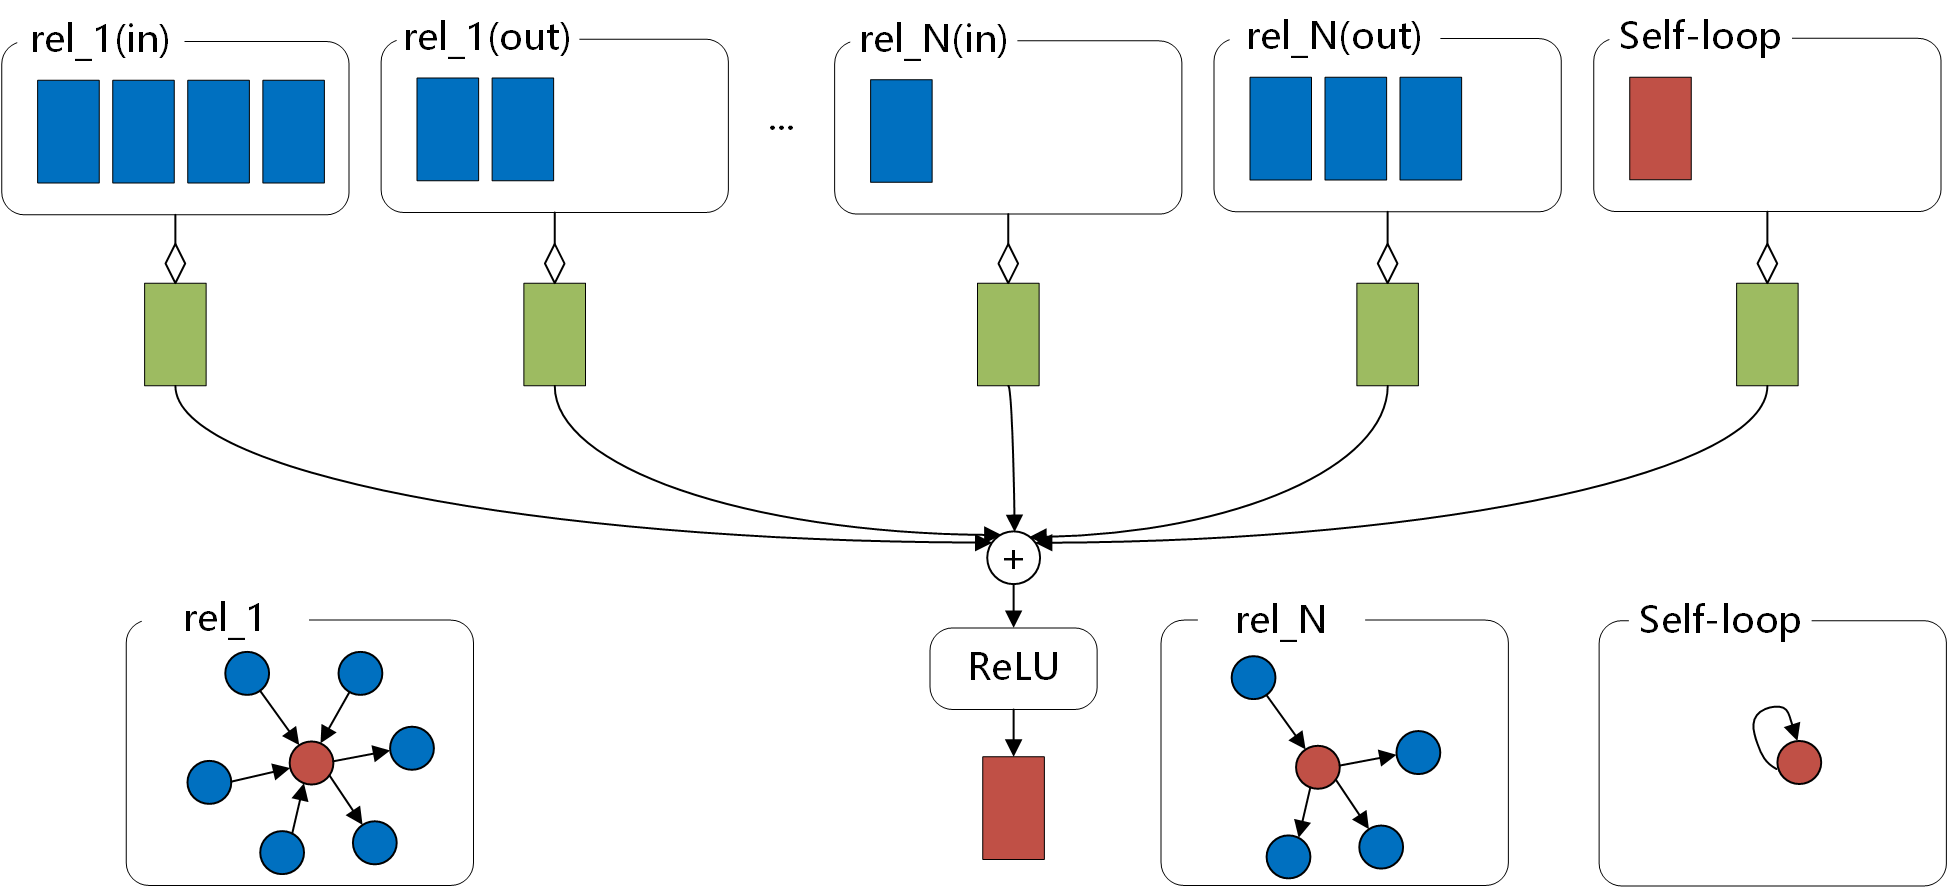
\includegraphics[width=.8\textwidth]{rgcn-cal.png}
    \caption{每层图网络隐状态更新过程\label{rgcn-cal}}
\end{figure}

每一层图网络的更新都需要对有向图中每个节点按照公式\ref{propo-in-directedgraph}进行并行计算。在模型实现中,可以堆叠多个图网络层以获取跨多个边的依赖关系。其中单个节点更新的计算图如图\ref{rgcn-cal}所示。待更新隐状态的结点或实体为红色,其所有的一跳邻居结点都为蓝色,用$d$维度的向量表示。然后针对每个relation类型分别进行信息传播计算,信息计算结果表示以标准化和的形式累加(绿色),最后经过激活函数作为新的隐状态向量,激活函数可以选择ReLU等。

\subsection{优化目标}
模型在进行参数更新时,主要使用了来自实体分类和链接预测两方面的损失函数。

实体分类:将如式子\ref{propo-in-directedgraph}的每一层图神经网络堆叠起来,并在最后一层节点的输出隐状态向量上使用$\operatorname{softmax}(\cdot)$激活函数。最终在标注的结点上最小化式\ref{node-class-crossenphory}表示的交叉熵损失函数即可。
\begin{equation}
    \mathcal{L}=-\sum_{i \in \mathcal{Y}} \sum_{k=1}^{K} t_{i k} \ln h_{i k}^{(L)}
    \label{node-class-crossenphory}
\end{equation}

其中$\mathcal{Y}$是有标签的结点索引集,$h_{i k}^{(L)}$是索引为$i$的带标签结点对应的网络输出的第$k$维的实数值。$t_{i k}$表示该实体的标注向量第$k$维的实数值。最后使用梯度下降算法训练模型参数即可。

链接预测:预测事实存在还是不存在(即三元组$(head,relation,tail)$是否存在)。有向、有标注的知识图谱可以使用符号式表示,即$G=(\mathcal{V}, \mathcal{E}, \mathcal{R})$。训练过程中没有使用完整的边集$\mathcal{E}$,而是使用了其子集$\hat{\mathcal{E}}$。模型会给候选边$(h, r, t)$一个分数$f(h, r, t)$,用以确定该边属于$\mathcal{E}$的可能性有多大。
为了进行链接预测,该文献引入了图编码-解码模型,编码部分使用上述图神经网络编码实体,解码部分对应着一个打分函数。编码器将每一个实体$v_{i} \in \mathcal{V}$映射到一个实数向量$e_{i} \in \mathbb{R}^{d}$。解码器会根据编码器输出的实体表示预测链接,具体实现上就是通过形如$s: \mathbb{R}^{d} \times \mathcal{R} \times \mathbb{R}^{d} \rightarrow \mathbb{R}$的函数给三元组$(head, relation, tail)$评分。编码器选用了上述的图卷积网络,解码器选用了文献\parencite{yang2014embedding}中的DistMult模型。DistMult模型中每一个关系$r$都与对角矩阵$R_{r} \in \mathbb{R}^{d \times d}$相关,候选三元组可以用式\ref{rgcn-link-score}计算得到评分。
\begin{equation}
    f(h, r, t)=e_{h}^{T} R_{r} e_{t}
    \label{rgcn-link-score}
\end{equation}
训练时,使用负采样为每个三元组负采样$\omega$个负样本。负样本来自于将正确的三元组的head或tail随机地替换掉。最终以正确的三元组评分要高于负样本为目的,使用了以下式\ref{rgcn-link-loss}为损失函数。

\begin{equation}
    \begin{aligned}
        \mathcal{L}=-\frac{1}{(1+\omega)|\hat{\mathcal{E}}|} & \sum_{(h, r, t, y) \in \mathcal{T}} y \log l(f(h, r, t))+\\
        &(1-y) \log (1-l(f(h, r, t)))
        \end{aligned}
    \label{rgcn-link-loss}
\end{equation}
其中$\mathcal{T}$是包含了正确和错误三元组的集合,而$l$是sigmoid函数。$y$是三元组的标签,$y=1$表示该三元组是正确的,$y=0$表示该三元组是错误的。在计算得到损失值后,会使用随机梯度下降算法更新模型参数。

\section{双向长短期记忆神经网络}\label{memory-net-section}
本节主要介绍编码时序数据的双向长短期记忆神经网络(Bi-directional Long Short-Term Memory,BiLSTM)。双向长短期记忆神经网络被广泛运用在许多场景中,本文以文献\parencite{gao2020task}中使用该模型进行故障预测为例,展开具体介绍。本节会进一步分为两小节分别介绍 BiLSTM 的模型结构和优化目标。
\subsection{模型结构}
\begin{figure}[htbp]
    \centering
    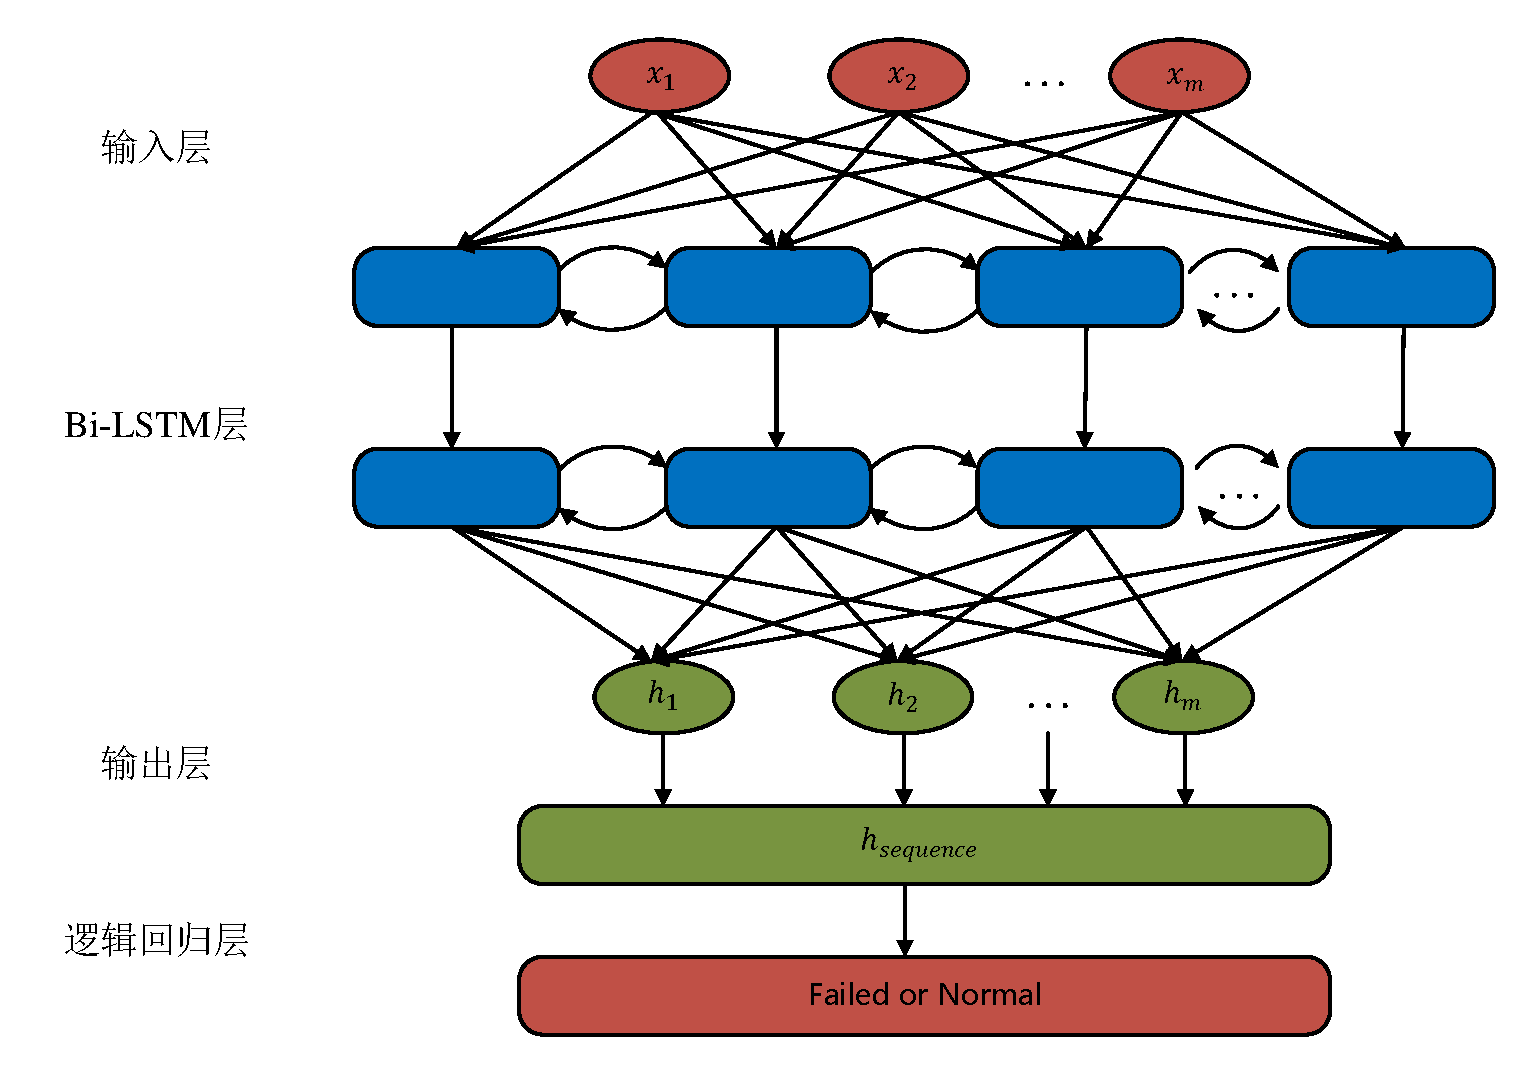
\includegraphics[width=.7\textwidth]{bilstm-model.pdf}
    \caption{基于双向长短期记忆神经网络的故障预测模型\label{bilstm-model}}
\end{figure}
图\ref{bilstm-model}所示为文献\parencite{gao2020task}用于故障预测的模型架构,可见其包含输入层、BiLSTM层、输出层和逻辑回归层。

输入层主要是数据的嵌入层。文献\parencite{gao2020task}拼接了同一时间点的CPU使用率、内存使用率、未映射页缓存、平均磁盘I/O时间、磁盘使用率、任务优先级、提交时间和提交次数共计8个特征。这样之后每个时间点都是一个8维的嵌入向量。
\begin{figure}[htbp]
    \centering
    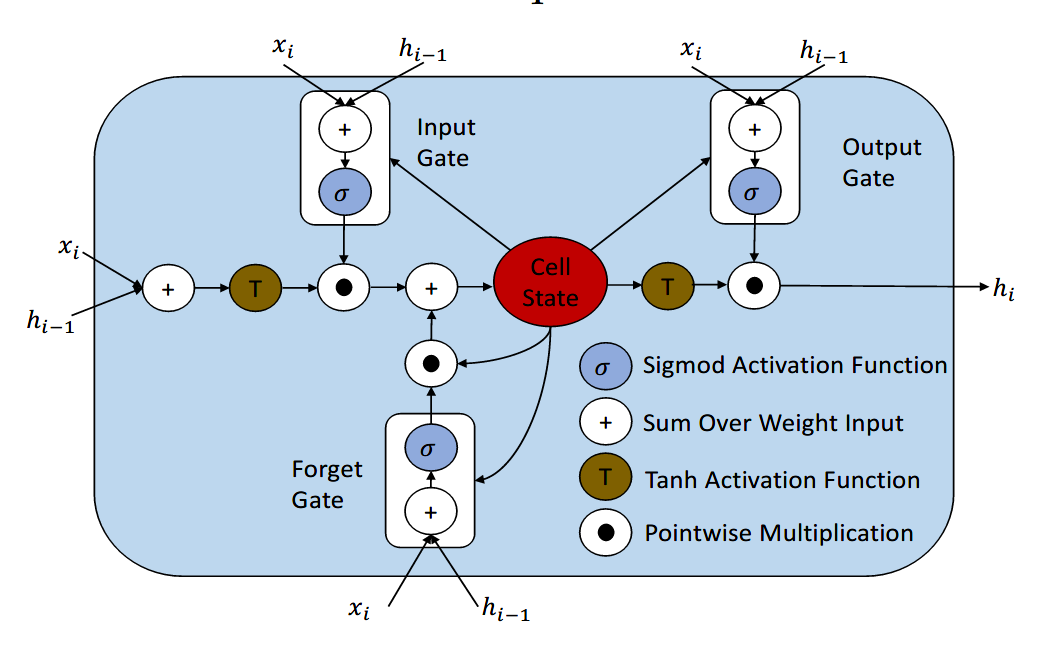
\includegraphics[width=.6\textwidth]{lstm-cell.png}
    \caption{双向长短期记忆网络神经单元\label{lstm-cell}}
\end{figure}

BiLSTM层完成了对时序数据的特征编码。该层会将输入的时序数据分别进行前向编码和后向编码,再将得到的前向隐状态和后向隐状态拼接得到最终的隐状态。经过上述步骤后,每个时间点的隐状态都会得到正向反向的上下文信息。图\ref{lstm-cell}展示了LSTM神经元内部的结构,可见其主要利用了非线性函数选择数据保存还是舍弃。具体实现上,每个神经元内部共有三个门控制其状态,包括输入门、遗忘门和输出门。输入门决定了应该更新哪个神经元状态,遗忘门决定了应该忽视掉什么信息,输出门决定输出隐状态的哪部分信息。该过程可以用公式\ref{lstm-cell-equation}表示:
\begin{equation}
    \begin{array}{l}
    g_{i}=\varphi\left(w_{g x} x_{i}+w_{g h} h_{i - 1}+b_{g}\right) \\
    n_{i}=\sigma\left(w_{n x} x_{i}+w_{n h} h_{i- 1}+b_{n}\right) \\
    f_{i}=\sigma\left(w_{f x} x_{i}+w_{f h} h_{i- 1}+b_{f}\right) \\
    o_{i}=\sigma\left(w_{o x} x_{i}+w_{o h} h_{i- 1}+b_{o}\right) \\
    s_{i}=g_{i} \odot n_{i}+s_{i -1} \odot f_{i} \\
    h_{i}=\varphi\left(s_{i}\right) \odot o_{i}
    \end{array}
    \label{lstm-cell-equation}
\end{equation}
其中$w_{gx}, w_{nx}, w_{fx} $和$w_{ox} $是记忆单元输入$x_{i}$的权重系数。$w_{gh}, w_{nh}, w_{fh} $和$w_{oh} $是记忆单元上一步输出$h_{i-1}$的权重系数。$b_{g}, b_{n}, b_{f},$ 和 $b_{o}$分别为输入信息$g_{i}$、输入门$n_{i}$、遗忘门$f_{i}$和输出门$o_{i}$对应的偏置系数。而$s_{i}$和$s_{i-1}$则分别为时间$i$和$i-1$的神经元状态。另外,$\odot$代表点乘,$\sigma$代表sigmoid激活函数,$\varphi$代表tanh激活函数。

输出层目的在于将输入序列中每个记忆单元隐状态整合起来。具体方式是将输入$X=\left\{x_{1}, x_{2} \ldots x_{m}\right\}$传入Bi-LSTM得到的表示序列$\left\{h_{1}, h_{2} \ldots h_{m}\right\}$进行式\ref{mean-pool}中所示的平均池化操作,得到序列表示向量$\widehat{h}$。
\begin{equation}
    \widehat{h}=\frac{1}{m} \sum_{i=1}^{m} h_{i}
    \label{mean-pool}
\end{equation}

逻辑回归层是预测当前数据序列将来是否会有故障的二分类层。具体实现上,该层将输出层得到的向量表示$\widehat{h}$输入$\operatorname{logstic}(.)$函数,计算会出现故障的概率。当概率大于阈值时,则预测会出现故障;反之,则预测不会出现故障。

\subsection{优化目标}
该模型的最终训练目标为正确分类每条数据序列。对应的损失函数为式\ref{memroy-net-loss}中所示。
\begin{equation}
    \mathcal{L}=-\sum_{i=1}^{n}\left[Y_{i} \log \left(f\left(X_{i} \right)\right)+\left(1-Y_{i}\right) \log \left(1-f\left(X_{i} \right)\right)\right]
    \label{memroy-net-loss}
\end{equation}

其中$X_{i}$表示第$i$条输入序列,$Y_{i}$为$X_{i}$对应的标签,即下一个时间点是否会有故障发生(1代表有故障发生,0代表不会有故障发生)。$f\left(.\right)$表示上文的BiLSTM模型。由损失函数计算得到损失值后,随机梯度下降会被用于更新模型参数。

\section{注意力机制}
注意力机制是一种自适应关注有效信息的机制,可以有效捕获长距离依赖信息\cite{mnih2014recurrent}。其本质上就是使用查询向量对一组键值向量计算权重分布,再根据权重分布对一组值向量加权平均。

注意力机制已经被广泛的应用在图像分类\cite{mnih2014recurrent}、神经机器翻译\cite{DBLP:conf/emnlp/LuongPM15}、多媒体推荐\cite{chen2017attentive}等领域。

在图像分类任务中,由于卷积神经网络的计算成本与输入图像的像素数成线性比例关系,因此在大图像上应用卷积神经网络的计算成本很高。为了解决巨大的计算成本问题,文献\parencite{mnih2014recurrent}提出了引入注意力机制的网络模型,所提出的模型自适应地从图像或视频中选择一系列区域,并且以高分辨率处理所选择的区域。

在机器翻译任务中,注意机制在翻译过程中有选择地聚焦于输入句子的有效部分,提高了机器翻译的准确性。Luong等人提出了两种机器翻译的注意机制方法:一种是始终关注所有源词的全局方法,另一种是只考虑源词子集的局部方法\cite{DBLP:conf/emnlp/LuongPM15}。

在多媒体推荐任务中,现有的协同过滤系统忽略了用户与多媒体内容间的隐含交互。文献\parencite{chen2017attentive}提出了两层注意机制来提取隐含交互。其中,底层自适应地选择组件级的隐含交互。上层自适应地选择项目级的隐含交互。两部分隐含交互会被结合起来输入经典的协同过滤模型。

\section{本章小结}
本章对本文中后续会涉及到的相关背景知识进行了介绍。本章首先介绍了支持向量机,支持向量机是进行分类的经典模型;其次介绍了关系图卷积神经网络,第四章会使用其获取实体上下文信息,实现组件-事件知识图谱实体的动态表示;随后介绍了双向长短期记忆神经网络,为第五章结合知识图谱和事件序列进行故障预测做了铺垫;最后介绍了注意力机制,第四章和第五章均使用其关注有效信息。
\chapter{组件-事件知识图谱构建}
目前已有的分布式集群运行状态监测模型都不能覆盖整合所有种类的信息。文献\parencite{wang2019grano}只构建了组件拓扑图而忽略了组件上数据之间的因果关系;文献\parencite{nie2016mining-causality-graph}将运行时信息转为事件数据后,只关注了事件间的因果图而忽略事件所在组件之间的拓扑关系;文献\parencite{qiu2020causality-mining-knowledge-graph}尝试构建运维知识图谱,但所构建的知识图谱只包含组件间的访问与部署关系、指标与组件间的来源产生关系,对于异常信息间的触发关系,只能精确到指标时序类型之间的因果关系,如“Container1 CPU usage”导致了“Microservice 1 Response Time”,不能进一步确定是什么样的 CPU 变化导致了什么样的响应时间变化。

为了解决上述多源异构数据难以覆盖整合的问题,本章提出了横跨硬件、软件、异常数据的组件-事件知识图谱构建方案。本章共分为5个小节展开介绍:首先,描述了组件-事件知识图谱构建的总体框架;其次,分3个小节分别介绍组件层信息获取,事件层信息获取和组件-事件知识图谱生成;最后模拟构建数据集,并对事件因果关系判别模型进行了实验分析。

% 对于组件部分数据,云服务商会提供开放的API返回分布式集群含有的组件属性信息、每类组件数量及每个组件间的关联关系。在事件层面,包含着分布式应用部署、模拟触发故障、数据收集、数据清洗、事件生成、事件因果关系挖掘及事件知识图谱构建。最后根据事件来源的组件类型,即可合并组件事件数据,构建生成组件-事件知识图谱。
\section{总体框架}
组件-事件知识图谱的总体构建框架如图\ref{kg-construct-total}所示。一方面,通过公开API(Application Programming Interface)和微服务追踪系统,获取组件唯一标识符、属性和关联关系,得到了组件层图谱;另一方面,将日志、指标时序数据等运行时信息转为了事件类型数据,然后引入了新的事件特征用于发掘事件间因果关系,得到了事件层图谱。最后,将同故障类型的组件层图谱、事件层图谱连接起来,自动沉淀出了标有对应故障类型的组件-事件知识图谱。
\begin{figure}[htbp]
    \centering
    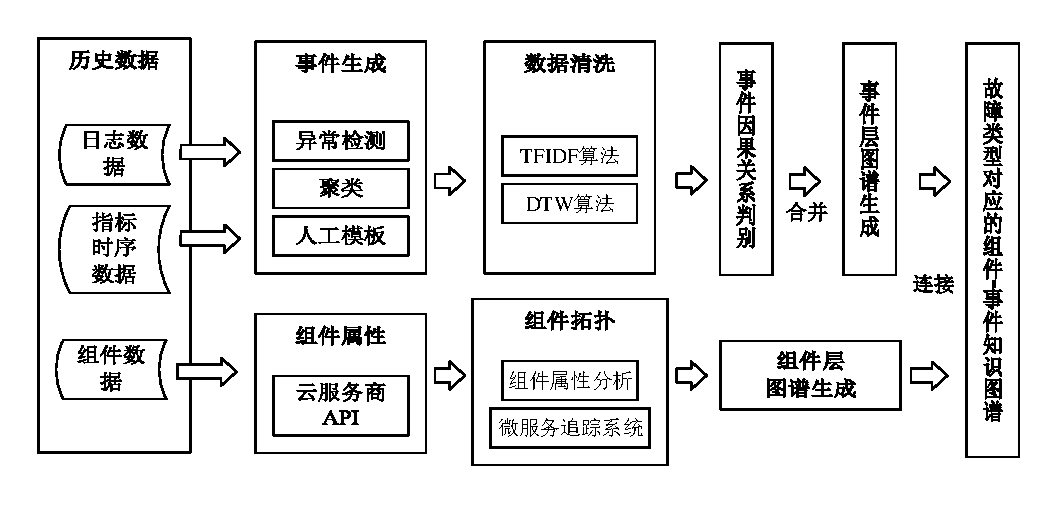
\includegraphics[width=.8\textwidth]{kg-construct-total.pdf}
    \caption{组件-事件知识图谱构建总体框架图\label{kg-construct-total}}
\end{figure}
\section{组件层信息获取}
% https://help.aliyun.com/document_detail/86742.html
Kubernetes(k8s)集群\cite{bernstein2014containers}在云计算行业中已经被广泛使用,它是一个具有扩展性、移植性的开源平台,同时具有着清晰的声明式配置和自动化特性,被用于管理各种容器化工作负载和服务。Kubernetes集群由一组工作机器(称为节点)组成,这些节点上运行着微服务,但为微服务并不是直接运行在这些节点上,而是由节点中承载的Pod来负载这些微服务。在生产环境中,集群通常运行着多个节点,从而提供容错性和高可用性。Kubernetes中所有组件都被绑定在一起,其间存在着复杂的负载、交互等关系。
% 图\ref{Kubernetes-components}为一个Kubernetes集群示意图,可见所有组件都被绑定在一起,其间存在着复杂的负载、交互等关系。
% \begin{figure}[htbp]
%     % https://kubernetes.io/zh/docs/concepts/architecture/cloud-controller/
%     \centering
%     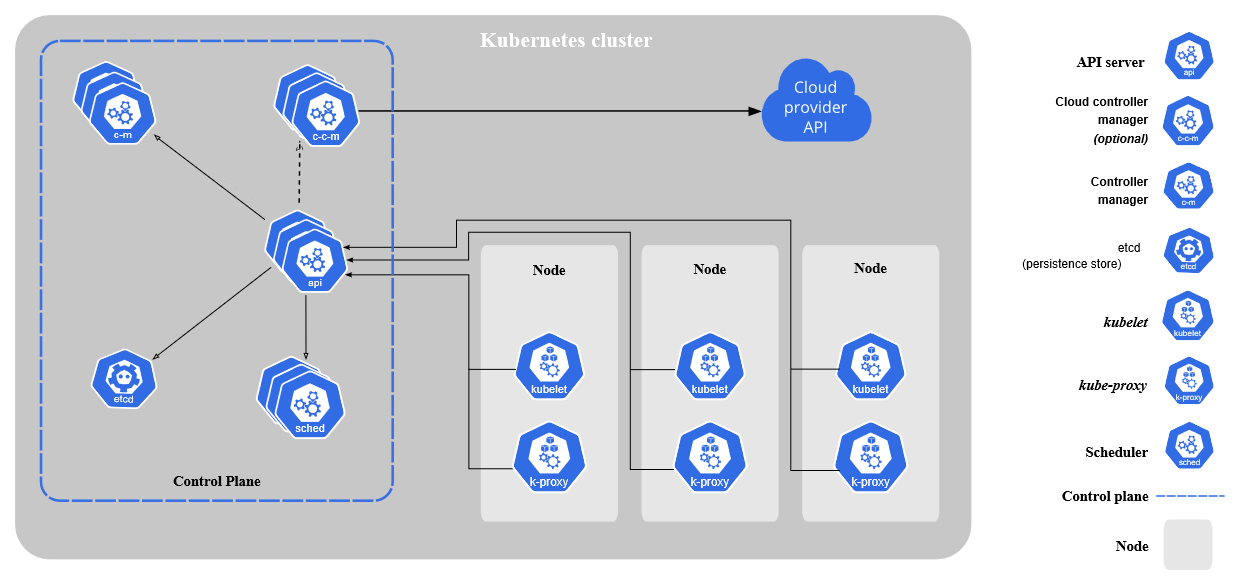
\includegraphics[width=.8\textwidth]{Kubernetes-components.png}
%     \caption{Kubernetes集群结构示意图\label{Kubernetes-components}}
% \end{figure}

本文所使用的Kubernetes集群是阿里云针对企业级应用所优化的容器服务版Kubernetes集群,其管理容器化应用的能力具有伸缩性,性能较高。阿里云对其提供的Kubernetes集群中各类组件都进行了清晰定义,具体上各类组件类型及含义如表\ref{systemCompotent}所示。
\newcommand{\tabincell}[2]{\begin{tabular}{@{}#1@{}}#2\end{tabular}}  
\begin{table}[htbp]
    \centering
    \caption{集群组件信息}
    \begin{tabular}{cc}
    \toprule[1.5pt]
        
        组件名称 & 含义 \\ \toprule[1.5pt]
        VPC & \tabincell{l}{专有网络(Virtual Private Cloud,VPC)是自定义私有网络。不同的专有网络之间\\存在二层逻辑隔离。用户可以在自己创建的专有网络内创建和管理各个云产品实\\例,比如ECS、SLB 、RDS 等。}  \\
        \midrule[1pt]
        SLB & \tabincell{l}{负载均衡器(Server Load Balancer,SLB)负责提供对多台应用实例进行流量分发\\的负载均衡服务。用户可以通过分流提高系统的服务能力,也可以通过消除单点\\故障使其具有可用性。} \\ 
        \midrule[1pt]
        ECS & \tabincell{l}{云服务器(Elastic Compute Service,ECS)是一种简单高效、具有弹性处理能力\\的计算服务。云服务器可以辅助用户高效率构建安全性、稳定性高的应用。} \\ 
        \midrule[1pt]
        Pod & \tabincell{l}{Pod 是 Kubernetes 中最小的部署单元和计费单位,根据应用场景,可以由一个或\\多个容器组成。当一个 Pod 中有多个容器时,这些容器会共享 Pod 的计算资源、\\存储空间、IP和端口。对于计算资源,Pod还可以限制各个容器使用的比例。} \\ 
        \midrule[1pt]
        Container & \tabincell{l}{Container即为容器,它包含在Pod中。一个Pod中有一个Pause容器和若干\\个业务容器。} \\ 
        \midrule[1pt]
        Service & \tabincell{l}{微服务是一种云原生架构方法,其中单个应用程序由许多松散耦合且可独立\\部署的较小Service组成。} \\ 
    
    \bottomrule[1.5pt]
    \end{tabular}
    \label{systemCompotent}
\end{table}
% 为了获取处于运行状态的Kubernetes集群中各个组件实例的唯一标识、属性和其间的关联关系,,以及所属VPC的Id信息

对于组件属性信息,本文使用了云服务商提供的公开API进行数据的请求,如获取某区域ECS属性信息的API为DescribeInstances(.)方法接口,输入地理区域“cn-hangzhou”,就会返回该区域的ECS信息。图\ref{api_ecs_info}为调用API后返回的杭州区域一台ECS的信息列表,包含该ECS的资源组、内存、唯一标识符、创建时间等属性信息。此外,VPC、SLB、Pod和Container都有着对应的API。在获取组件属性时,本文分别调用不同的API设定不同参数,最终可以获取到同一集群内所有组件的属性信息。

对于组件间拓扑关系,VPC、SLB、ECS、Pod和Container间的拓扑关系可以通过分析属性信息获取,而Service间的拓扑则需要借助微服务追踪系统获取。同样以图\ref{api_ecs_info}为例,返回信息中VpcId字段就表明了该ECS位于id为“vpc—2zeuphj 08tt7q3brd****”的虚拟私有网络下。除了Service类型组件,所有集群组件均可通过分析API返回的属性信息,获取到与其他组件的关联信息。Service类型组件对应着部署在Kubernetes集群中的分布式应用的各个微服务。微服务之间的拓扑关系与开发人员编写的应用架构有关,无法通过云服务商提供的公开API直接获取。另外,分布式应用代码是其所属公司的保密性数据,不能被外部获取或改写,所以通过侵入代码获取微服务结构的方法是不可行的。目前开放式的微服务追踪系统(如Jaeger\cite{mengistu2020distributed}),可以跟踪微服务之间的请求数据,然后分析汇总这些请求链路就可以构建出微服务之间的访问拓扑关系。追踪请求数据生成微服务拓扑关系的方法不必侵入代码,也不需要运维人员阅读分布式应用的开发文档,只需要将追踪系统部署在分布式应用所在的集群中跟踪分布式应用即可。

综上,本文通过云服务商提供的公开API和微服务追踪系统,获取了组件部分的实体属性及拓扑结构。
\begin{figure}[htbp]
    \centering
    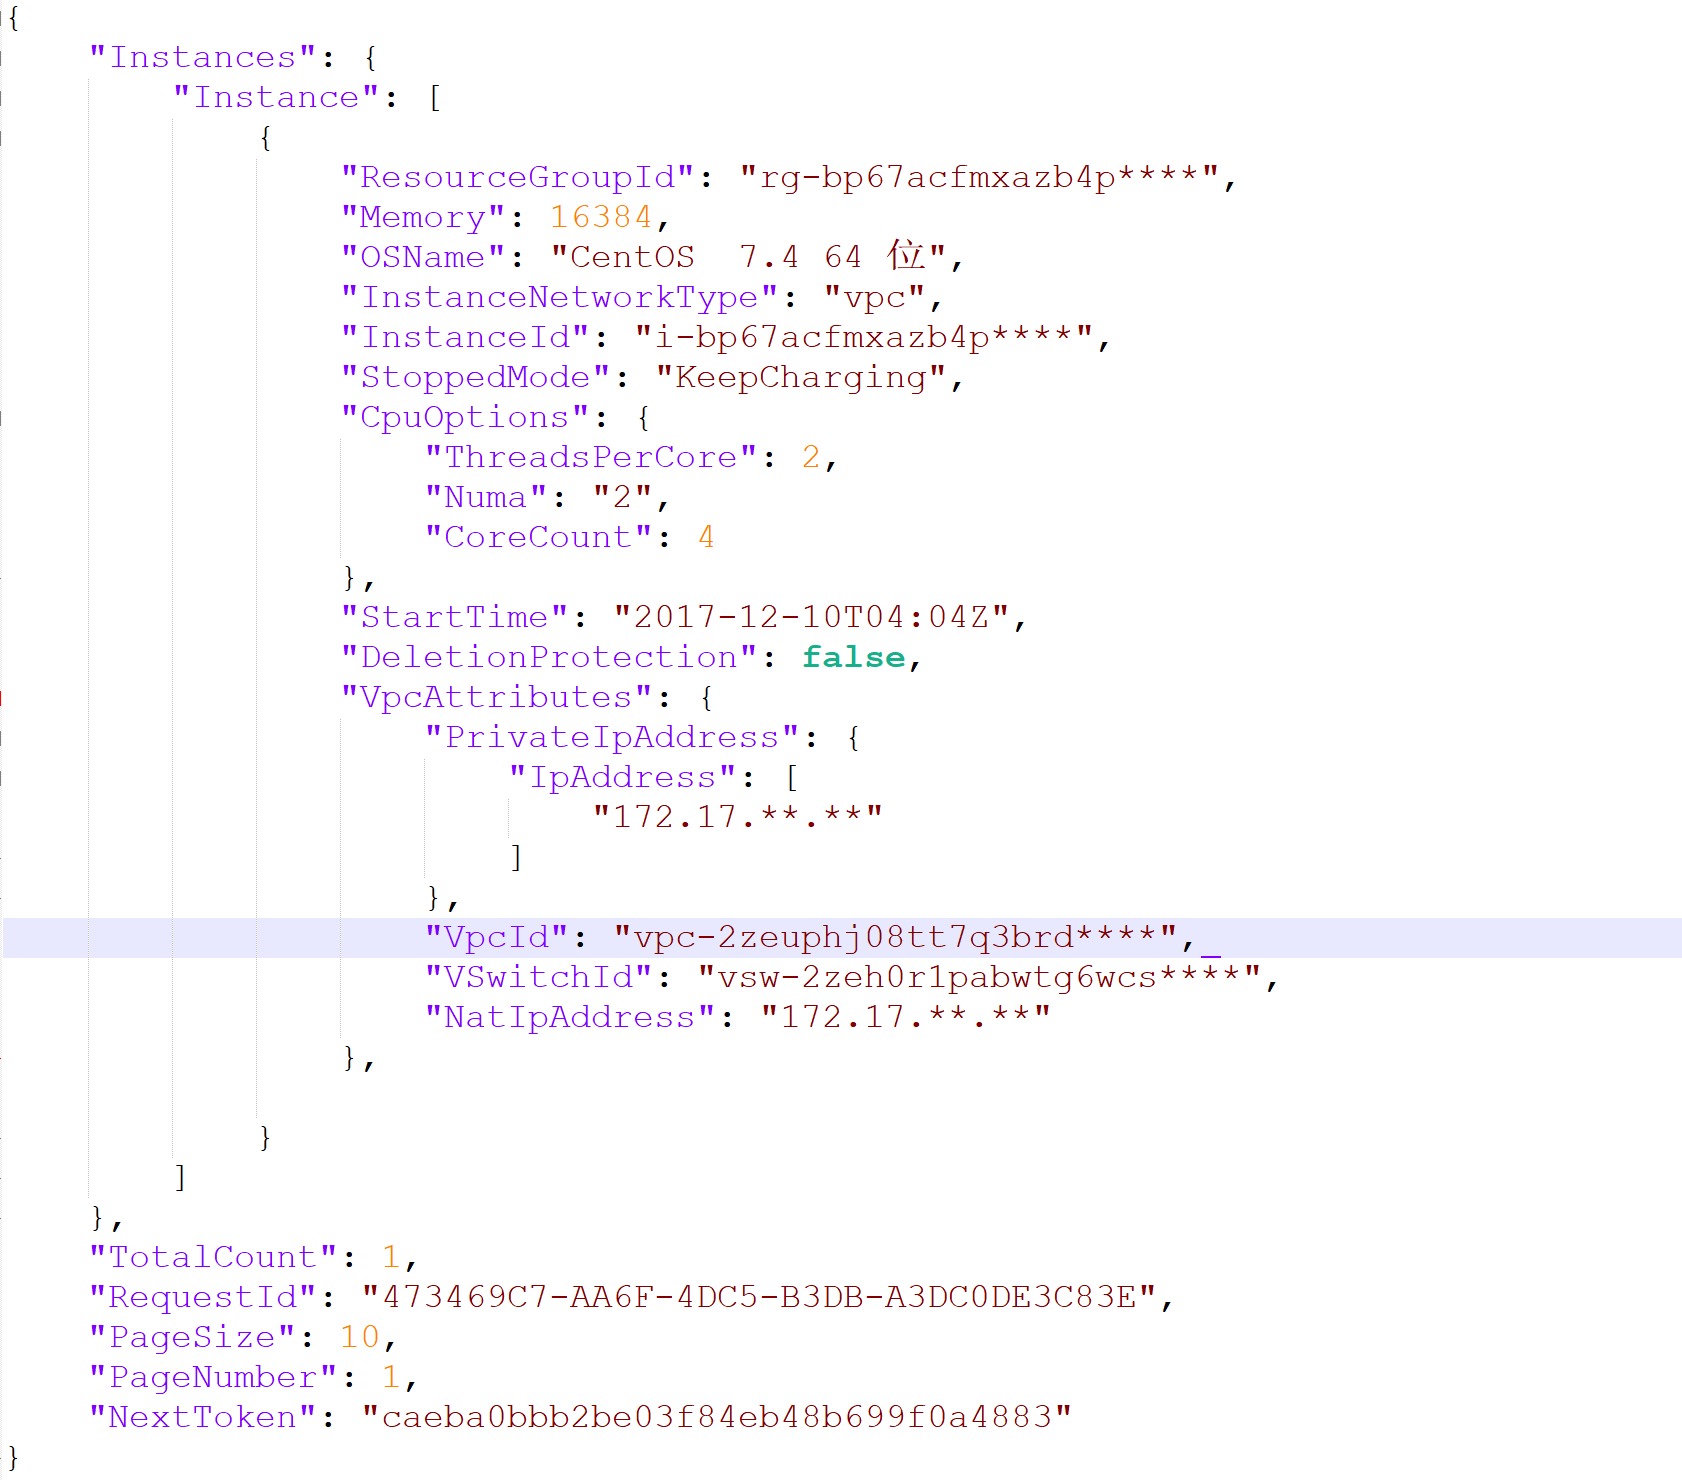
\includegraphics[width=.8\textwidth]{api_ecs_info.png}
    \caption{阿里云公开API返回ECS数据部分示例\label{api_ecs_info}}
\end{figure}

\section{事件层信息获取}
本小节旨在将集群运行状态数据经过清洗整理后转为事件信息,并进一步经过关系分类器挖掘事件间因果关系。本小节分为两部分展开介绍,分别为事件生成和事件因果关系挖掘。

在事件生成部分,使用了聚类、异常识别、模板匹配结合的方式,将实时产生的日志、指标时序数据转为了事件类数据。

在事件因果关系挖掘部分,过往工作大量依赖基于概率的事件特征,导致领域专家需要反复标注海量数据训练模型才能达到良好效果。为了克服该问题,本文设计并引入了新的事件特征,最终不需要反复标注海量数据就可以达到优质的效果。
\subsection{事件生成}\label{event-generate}
\begin{definition}[事件]
    \label{event-define}
    事件。事件是对分布式系统中组件运行状态的描述。主要包括五个部分:
    {\\\qquad
        Id:事件的唯一标识;\\
        Time:事件发生的时间戳;\\\qquad
        Location:事件发生所在的具体组件;\\\qquad
        EventType:事件类型描述;\\\qquad
        Detail:事件的具体描述\\\qquad
    }
\end{definition}

\begin{definition}[完全周期性事件]
    \label{periodic-event}
    完全周期性事件是严格按照一定时间间隔出现的事件,如每隔3s必然出现一次。
\end{definition}

事件定义如Definition \ref{event-define}所示。在生成事件之前,需要先收集到指标时序数据、日志数据。本文部署了云计算相关工作常用的两个开源应用train-ticket\cite{zhou2018poster} 、sock-shop\cite{rahman2019predicting}于阿里云平台上,随后分别多次模拟了常见的故障,并收集了两个应用正常数据以及各个故障场景的异常数据。具体数据收集情况会在实验部分详细描述。
\begin{figure}[htbp]
    \centering
    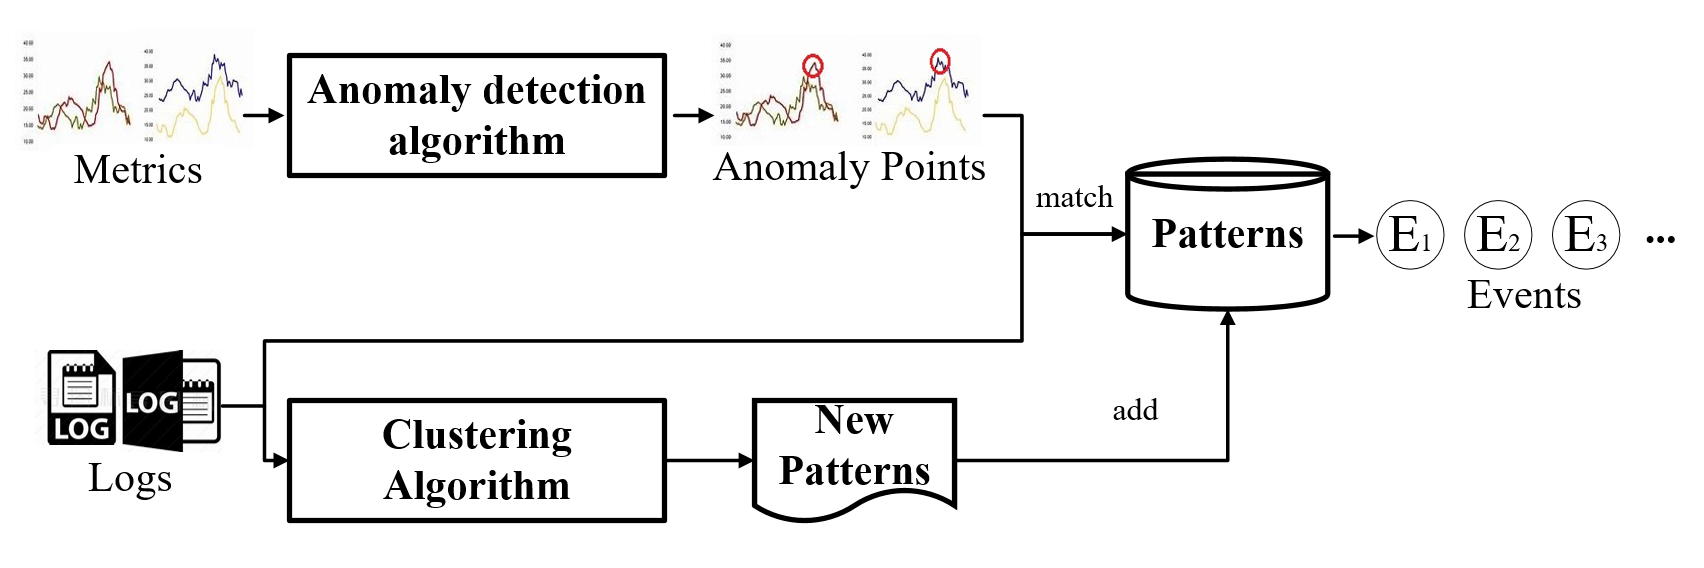
\includegraphics[width=.8\textwidth]{event-generate.png}
    \caption{事件生成流程\label{event-generate}}
\end{figure}

在收集完相关原始数据后,事件生成模块的主要功能是将系统的异常信息转为统一规范的事件数据,整体流程如图\ref{event-generate}所示。系统中的数据主要有两种,一种是指标时序数据,记录着系统各个组件的状态曲线变换,如内存、读写、CPU等随时间的变化曲线;另一种是日志数据,记录着微服务在具体时间戳打印的日志内容,如在某个时间微服务打印“xxx service strats success”日志。

对于指标时序数据,本文首先使用异常检测算法检测到异常点,比如某些指标开始很平滑,然后经过某个点后开始抖动,那么这个转折点就是异常点,异常点一般是系统发生异常的一种表现。在找到异常点后,经过模板匹配就可以得到异常事件。比如某Container的CPU使用率曲线突然上升到100\%,那么根据模板可以得到这个异常点事件类型是“container.cpu.usage.seconds.total”。对于日志数据,一方面会使用聚类算法发掘日志中的通用模板,如果有新模板产生,那么就会添加到模板库中;另一方面会使用模板库中的模板来匹配日志生成相应事件。图\ref{log-example}中是一些日志数据,这些日志由于格式比较类似,相同的关键词也比较多,因此会被聚类算法分为一类,这一类的模板就会写为 “****-**-** **:**:**, pod *** occurs Back-off restarting failed”,随后这个模板会被添加到模板库中,之后产生的日志匹配到此类模板会生成相应的事件。上文提到的异常检测算法\cite{yang2019integrated}和聚类算法\cite{landauer2020system}目前业界已有很多,不是本文主要研究内容,所以这里就不展开对这方面的细致介绍。
\begin{figure}[htbp]
    \centering
    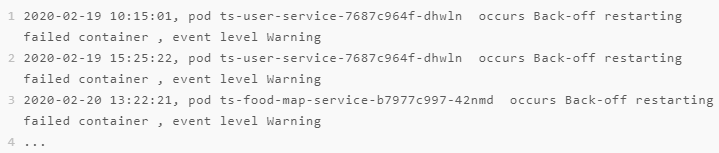
\includegraphics[width=.85\textwidth]{log-example.png}
    \caption{日志数据样例\label{log-example}}
\end{figure}

此外,在生成的事件中存在大量的完全周期性事件,其定义如Definition \ref{periodic-event}所示。完全周期性事件的存在,一方面使得事件数量级抖升而增加了时空复杂度,一方面会干扰后续事件因果分析、故障预测的效果。完全周期性事件不管集群有无异常都会保持绝对的周期出现,与集群状态无关。因此,在生成事件后,需要初步筛选去除具有完全周期性的事件,本文使用DTW(Dynamic Time Warping)算法\cite{mueen2016extracting}判断事件是否为完全周期性事件。采用DTW算法的原因在于该算法已经在语音匹配任务中取得了优秀的效果,它不需要曲线精确的对位分析,能适应时间错位性。利用该算法去除完全周期性噪声事件的具体做法为:

(1)统计某类事件$e$在异常注入前$t_1$时间段、异常到故障产生时间段$t_2$和故障发生后$t_{3}$时间段这三段时间内,发生的频次曲线。其中$t_1 = t_2 = t_3$。

(2)对比三段时间$t_1$、$t_2$和$t_{3}$所对应的三条频次曲线。如果DTW算法判别三者等同,则认为该类事件是完全周期性事件。

(3)对异常注入到故障产生时间段内的所有事件均采取上述判别过程。最终将认定有完全周期性的事件删除,只保留非完全周期性事件。该过程可以删去总事件量中约15\%的完全周期性事件,如在总共收集到的3738条事件中,删去了537条完全周期性事件。

本文生成的事件数据按照来源划分,可以分成两类:指标时序事件和日志事件。指标时序事件和日志事件可以继续往下划分,所划分生成的类别与每类别的数目如表\ref{event-type-level}所示。
% \vspace{-1.5cm}
% \begin{table}[htbp]
%     \caption{事件类型层次关系}
%     \centering
%     \label{event-type-level}
%     \begin{tabular}{cccc}
%     \toprule[1.5pt]
%     事件大类别    & 细分           & \begin{tabular}[c]{@{}c@{}}类别数目\\ (train-ticket)\end{tabular} & \begin{tabular}[c]{@{}c@{}}类别数目\\ (sock-shop)\end{tabular} \\ \midrule[1.5pt]
%     指标时序事件 & 异常点事件        & 64                 & 64              \\
%              & 告警事件         & 21                 & 21              \\ \midrule[1pt]
%     日志事件    & k8s日志事件      & 50                 & 50              \\
%              & dockerIO日志事件 & 69                 & 76              \\ \midrule[1pt]
%     共计       &              & 204                & 211             \\ 
%     \bottomrule[1.5pt]
%     \end{tabular}
% \end{table}
% Please add the following required packages to your document preamble:
% \usepackage{multirow}
\begin{table}[htbp]
    \centering
    \caption{事件类型层次关系}
    \label{event-type-level}
    \begin{tabular}{cccc}
    \toprule[1.5pt]
    事件大类别                   & 细分           & \begin{tabular}[c]{@{}c@{}}类别数目\\ (train-ticket)\end{tabular} & \begin{tabular}[c]{@{}c@{}}类别数目\\ (sock-shop)\end{tabular} \\ \midrule[1.5pt]
    \multirow{2}{*}{指标时序事件} & 异常点事件        & 64                                                            & 64                                                         \\
                            & 告警事件         & 21                                                            & 21                                                         \\ \midrule
    \multirow{2}{*}{日志事件}   & k8s 日志事件     & 50                                                            & 50                                                         \\
                            & dockerIO日志事件 & 69                                                            & 76                                                         \\ \midrule
    共计                      &              & 204                                                           & 211                                                        \\ \bottomrule[1.5pt]
    \end{tabular}
\end{table}
% \vspace{-1.5cm}

其中,异常点事件名称由监控项拼接异常点类型构成,表示了在组件的某个监控项曲线出现了某种异常点。监控项共有16种,如表\ref{kpi-event}所示。异常点类型共有4种:突然上升、突然下降、尖峰、低谷。每个监控项都会出现这四种异常点,比如$system.mem.util$突然上升$system.mem.util$突然下降、$system.mem.util$出现尖峰、$system.mem.util$出现低谷。因此,将每个监控项与异常点类型两两排列组合,可生成共计64种异常点事件。
% \begin{equation}
%     \begin{array}{l}
        % container.cpu.load.average.10s,\\
        % container.cpu.usage.seconds.total,\\
        % container.fs.reads.bytes.total,\\
        % container.fs.writes.bytes.total,\\
        % container.memory.usage.bytes,\\
        % container.network.receive.bytes.total,\\
        % container.network.receive.packets.dropped.total,\\
        % container.network.transmit.bytes.total,\\
        % container.network.transmit.packets.dropped.total,\\
        % system.net.drop.util,\\
        % system.net.in,\\
        % system.net.out,\\
        % system.io.disk.rbps,\\
        % system.io.disk.wbps,\\
        % system.mem.util,\\
        % system.cpu.util\\ 
%     \end{array}
%     \label{kpi-event}
% \end{equation}
\newpage
\begin{table}[htbp]
    \centering
    \caption{异常事件监控项列表}
    \label{kpi-event}
    \begin{tabular}{c}
    \toprule[1.5pt]
    监控项名称                                         \\ \midrule[1.5pt]
    container.cpu.load.average.10s                   \\
    container.cpu.usage.seconds.total                \\
    container.fs.reads.bytes.total                   \\
    container.fs.writes.bytes.total                  \\
    container.memory.usage.bytes                     \\
    container.network.receive.bytes.total            \\
    container.network.receive.packets.dropped.total  \\
    container.network.transmit.bytes.total           \\
    container.network.transmit.packets.dropped.total \\
    system.net.drop.util                             \\
    system.net.in                                    \\
    system.net.out                                   \\
    system.io.disk.rbps                              \\
    system.io.disk.wbps                              \\
    system.mem.util                                  \\
    system.cpu.util                                  \\ \bottomrule[1.5pt]
    \end{tabular}
    \end{table}
% \begin{lstlisting}[xleftmargin=12em,label=code]
%     container.cpu.load.average.10s,
%     container.cpu.usage.seconds.total,
%     container.fs.reads.bytes.total,
%     container.fs.writes.bytes.total,
%     container.memory.usage.bytes,
%     container.network.receive.bytes.total,
%     container.network.receive.packets.dropped.total,
%     container.network.transmit.bytes.total,
%     container.network.transmit.packets.dropped.total,
%     system.net.drop.util,
%     system.net.in,
%     system.net.out,
%     system.io.disk.rbps,
%     system.io.disk.wbps,
%     system.mem.util,
%     system.cpu.util
% \end{lstlisting}

告警事件名称是由监控项和阈值组成的,表明了在设备的某个监控项上出现了达到阈值的告警信息。会发生告警事件的监控项共7种,每个监控项目都有3种告警阈值。监控项和相应阈值如表\ref{alarm-event}所示。可见每个监控项都会生成3种告警事件,比如$pod.cpu.util$达到$100\%$、$pod.cpu.util$达到$90\%$、$pod.cpu.util$达到$95\%$。因此,将每个监控项与对应阈值组合,可生成告警事件共计21种。
% \begin{table}[htbp]
%     \centering
%     \caption{告警事件监控项及相应阈值}
%     \label{alarm-event}
%     \begin{tabular}{cc}
%     \toprule[1.5pt]
%     监控项                          & 阈值              \\ \\\midrule[1.5pt]
%     pod.cpu.util                 & 100\% 95\% 90\% \\
%     pod.mem.util                 & 100\% 95\% 90\% \\
%     system.cpu.util              & 100\% 95\% 90\% \\
%     system.mem.util              & 100\% 95\% 90\% \\
%     system.net.drop.util         & 20\% 10\% 5\%   \\
%     system.net.err.util          & 20\% 10\% 5\%   \\
%     system.partition.space.usage & 100\% 95\% 90\% \\ 
%     \bottomrule[1.5pt]
%     \end{tabular}
%     \end{table}
\begin{table}[htbp]
    \centering
    \caption{告警事件监控项及相应阈值}
    \label{alarm-event}
    \begin{tabular}{cc}
    \toprule[1.5pt]
    监控项                          & 阈值              \\ \midrule[1.5pt]
    pod.cpu.util                 & 100\% 95\% 90\% \\
    pod.mem.util                 & 100\% 95\% 90\% \\
    system.cpu.util              & 100\% 95\% 90\% \\
    system.mem.util              & 100\% 95\% 90\% \\
    system.net.drop.util         & 20\% 10\% 5\%   \\
    system.net.err.util          & 20\% 10\% 5\%   \\
    system.partition.space.usage & 100\% 95\% 90\% \\ \bottomrule[1.5pt]
    \end{tabular}
\end{table}

k8s(kubeneters)是分布式集群容器的管理系统,k8s日志事件就是k8s管理系统产生的事件,包含pod镜像拉取、pod健康状况等事件。这类事件共有50种细分类型,表\ref{k8s-event}展示了部分k8s日志事件类型。
% \begin{lstlisting}[xleftmargin=12em,label=code]
%             Unhealthy.Warning,
%             Killing.Normal,
%             Scheduled.Normal,
%             Pulled.Normal,
%             Created.Normal,
%             Started.Normal,
%             Pulling.Normal,
%             BackOff.Warning,
%             FailedSync.Warning,
%             Failed.Warning,
%             FailedCreatePodSandBox.Warning,
%             SandboxChanged.Normal,
%             FailedKillPod.Warning,
%             FailedScheduling.Warning,
%             BackOff.Normal,
%             FailedMount.Warning,
%             Scheduled.Normal,
%             Pulled.Normal,
% \end{lstlisting}
% \begin{equation}
%     \begin{array}{c}
%         Unhealthy.Warning, \\
%         Killing.Normal,\\
%         Scheduled.Normal,\\
%         Pulled.Normal,\\
%         Created.Normal,\\
%         Started.Normal,\\
%         Pulling.Normal,\\
%         BackOff.Warning,\\
%         FailedSync.Warning,\\
%         Failed.Warning,\\
%         FailedCreatePodSandBox.Warning,\\
%         SandboxChanged.Normal,\\
%         FailedKillPod.Warning,\\
%         FailedScheduling.Warning,\\
%         BackOff.Normal,\\
%         FailedMount.Warning,\\ 
%         Scheduled.Normal,\\
%         Pulled.Normal,\\
%     \end{array}
%     \label{k8s-event}
% \end{equation}
\newpage
\begin{table}[thbp]
    \centering
    \caption{部分k8s日志事件类型}
    \label{k8s-event}
    \begin{tabular}{c}
    \toprule[1.5pt]
    k8s日志事件类型名                     \\ \midrule[1.5pt]
    Unhealthy.Warning              \\
    Killing.Normal                 \\
    Scheduled.Normal               \\
    Pulled.Normal                  \\
    Created.Normal                 \\
    Started.Normal                 \\
    Pulling.Normal                 \\
    BackOff.Warning                \\
    FailedSync.Warning             \\
    Failed.Warning                 \\
    FailedCreatePodSandBox.Warning \\
    SandboxChanged.Normal          \\
    FailedKillPod.Warning          \\
    FailedScheduling.Warning       \\
    BackOff.Normal                 \\
    FailedMount.Warning            \\
    Scheduled.Normal               \\
    Pulled.Normal                  \\ \bottomrule[1.5pt]
    \end{tabular}
\end{table}

DockerIO日志事件指的是Docker中的输入输出日志所转化生成的事件。该类事件记录了Docker\cite{boettiger2015introduction}中的各种操作信息和容器中微服务应用运行时日志信息。在将这些日志聚类并编写人工模板后,人工模板被用来匹配日志信息以收集统计DockerIO日志事件类型。其中,因为不同分布式应用的微服务结构不同,且输出日志直接由开发人员编写的代码所决定,所以两应用中的DockerIO事件类型有所不同。最终train-ticket应用中收集到69种DockerIO日志事件,而sock-shop应用中共收集到76种DockerIO日志事件。式\ref{dockerio-event}中列出了部分DockerIO日志事件类型名称。
% \begin{equation}
%     \begin{array}{l}
%         java.lang.AbstractMethodError,\\
%         java.lang.AssertionError,\\
%         java.lang.ClassCircularityError,\\
%         java.lang.ClassFormatError,\\
%         java.lang.Error,\\
%         spring.server.connect.failed,\\
%         warn.Omitting,\\
%         warning.stderr,\\
%         spring.http.server.error,\\
%         error.mcp.Failed.to.create.a.new.MCP.sink.stream,\\
%         trying.to.establish.new.MCP.sink.stream,\\
%         socket.go.Successful.write.metrics.to.monitor.server,\\
%         operator.go.sync.prometheus,\\
%         event.go.reason.UPDATE.Ingress,\\
%     \end{array}
%     \label{dockerio-event}
% \end{equation}
% \begin{lstlisting}[xleftmargin=12em,label=code]
%         java.lang.AbstractMethodError,
%         java.lang.AssertionError,
%         java.lang.ClassCircularityError,
%         java.lang.ClassFormatError,
%         java.lang.Error,
%         spring.server.connect.failed,
%         warn.Omitting,
%         warning.stderr,
%         spring.http.server.error,
%         error.mcp.Failed.to.create.a.new.MCP.sink.stream,
%         trying.to.establish.new.MCP.sink.stream,
%         socket.go.Successful.write.metrics.to.monitor.server,
%         operator.go.sync.prometheus,
%         event.go.reason.UPDATE.Ingress,
% \end{lstlisting}

% 本文生成的事件按照严重等级可以划分如表\ref{event-type}所示,包括正常事件、异常事件和故障事件。正常事件是指系统内组件在正常业务逻辑中产生的事件,注意正常事件也有可能引发故障,比如事件“服务器正在重启”,虽然此事件是服务器正常重启产生的事件,但是如果在此服务器重启时,其他服务器对其访问,也会产生“访问失败”事件,触发系统故障。异常事件是指系统组件发生了正常执行业务时不会出现的事件,如异常检测算法检测到的系统异于常态的事件,但异常事件发生时组件仍可工作,不会发生系统不可用。故障事件是描述组件故障的事件,故障事件发生时系统部分服务已无法正常工作。
% % Please add the following required packages to your document preamble:
% % \usepackage{multirow}
% % Please add the following required packages to your document preamble:
% % \usepackage{multirow}
% \begin{table}[htbp]
%     \centering
%     \caption{事件严重程度划分结果}
%     \label{event-type}
%     \begin{tabular}{ccc}
%     \toprule[1.5pt]
%     初级划分                  & 次级划分   & 示例                                                                                                       \\ 
%     \midrule[1pt]
%     \multirow{2}{*}{正常事件} & 硬件正常事件 & container memory 50\%、container cpu 50\%、...                                                             \\
%                           & 软件正常事件 & 数据库连接成功、...                                                                                              \\ 
%                           \midrule[1pt]
%     \multirow{2}{*}{异常事件} & 硬件异常事件 & container memory 100\%、container cpu 100\%、...                                                           \\
%                           & 软件异常事件 & 数据库连接失败、...                                                                                              \\ 
%                           \midrule[1pt]
%     \multirow{2}{*}{故障事件} & 硬件故障事件 & 服务器宕机、...                                                                                                \\
%                           & 软件故障事件 & \begin{tabular}[c]{@{}c@{}}HttpServerErrorException 503、\\ HttpServerErrorException 500、...\end{tabular} \\ 
%                           \bottomrule[1.5pt]
%     \end{tabular}
% \end{table}

% \begin{table}[]
%     \caption{事件严重程度划分}
%     \label{event-type}
%     \begin{tabular}{llll}
%     \hline
%     事件 & 正常事件 & 硬件正常事件 & container memory 50\%、container cpu 50\%、...                  \\
%        &      & 软件正常事件 & 数据库连接成功、...                                                   \\ \cline{2-4} 
%        & 异常事件 & 硬件异常事件 & container memory 100\%、container cpu 100\%、...                \\
%        &      & 软件异常事件 & 数据库连接失败、...                                                   \\ \cline{2-4} 
%        & 故障事件 & 硬件故障事件 & 服务器宕机、...                                                     \\
%        &      & 软件故障事件 & HttpServerErrorException 503、HttpServerErrorException 500、... \\ \hline
%     \end{tabular}
% \end{table}


% \begin{figure}[htbp]
%     \centering
%     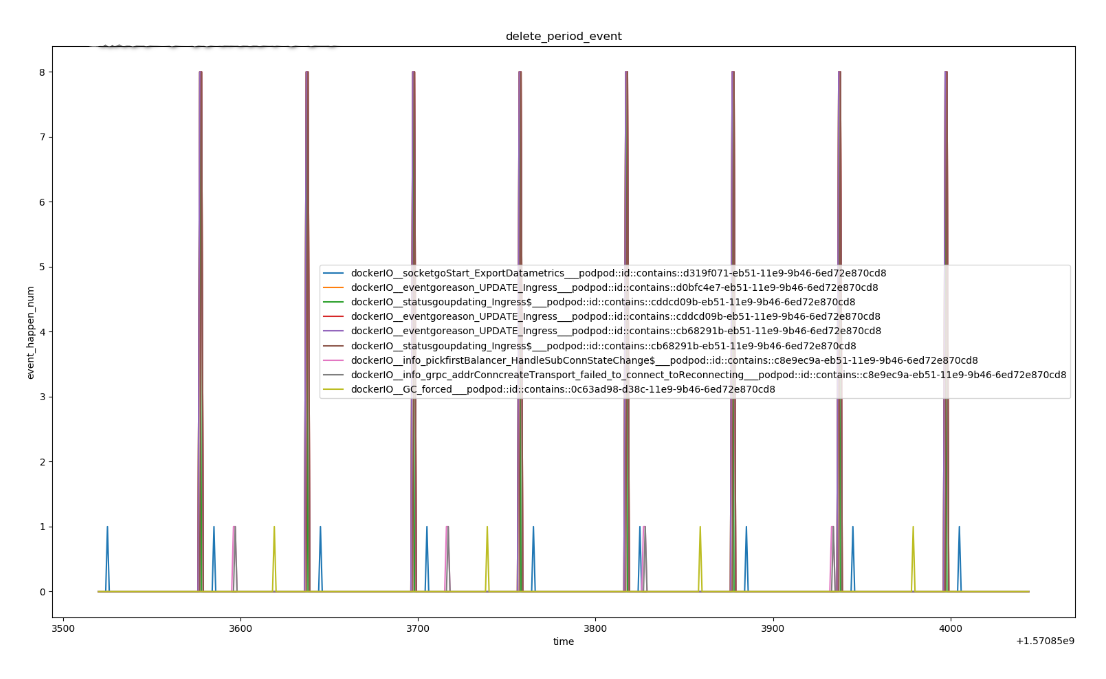
\includegraphics[width=.65\textwidth]{deleted-period-events.png}
%     \caption{筛去的完全周期性事件频次图\label{deleted-period-events}}
% \end{figure}

% 图\ref{saved-no-period-events}为保留的非完全周期性事件频次图。图\ref{deleted-period-events}为筛去的完全周期性事件频次图。可见被删去的完全周期性事件,均为集群管理系统发生的事件,如socket信息、垃圾回收信息和周期性更新信息等。

% \begin{figure}[htbp]
%     \centering
%     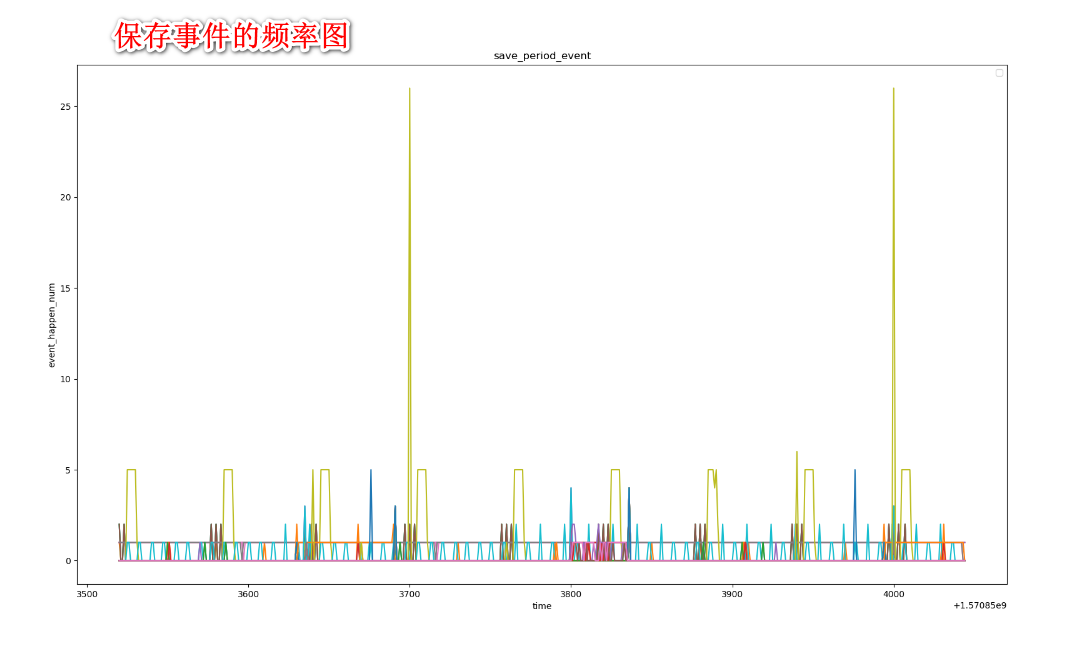
\includegraphics[width=.65\textwidth]{saved-no-period-events.png}
%     \caption{保留的非完全周期性事件频次图\label{saved-no-period-events}}
% \end{figure}
% \newpage
\subsection{事件因果关系挖掘}
关系分类器用于判别事件间关系类型,本文中为有无因果关系。输入关系分类器的是A、B两事件特征向量,输出为A到B是否有因果关系,即A→B是否存在。若要判断有无B到A(即B→A)的因果关系,需要按照顺序输入B、A两事件特征向量。本文共使用了以下6种事件特征,其中(1)(2)源自相关工作\cite{nie2016mining-causality-graph},(3)-(6)为本文新设计的事件特征。
\newpage
\begin{table}[htbp]
    \centering
    \caption{部分DockerIO日志事件类型}
    \label{dockerio-event}
    \begin{tabular}{c}
    \toprule[1.5pt]
    DockerIO日志事件类型                                       \\ \midrule[1.5pt]
    java.lang.AbstractMethodError                        \\
    java.lang.AssertionError                             \\
    java.lang.ClassCircularityError                      \\
    java.lang.ClassFormatError                           \\
    java.lang.Error                                      \\
    spring.server.connect.failed                         \\
    warn.Omitting                                        \\
    warning.stderr                                       \\
    spring.http.server.error                             \\
    error.mcp.Failed.to.create.a.new.MCP.sink.stream     \\
    trying.to.establish.new.MCP.sink.stream              \\
    socket.go.Successful.write.metrics.to.monitor.server \\
    operator.go.sync.prometheus                          \\
    event.go.reason.UPDATE.Ingress                       \\ \bottomrule[1.5pt]
    \end{tabular}
\end{table}

(1) 皮尔逊相关系数:该特征用来计算两个事件之间的相关性,即两个事件之间的皮尔逊相关系数越高,那么这两个事件越相关,越有可能是因果关系。皮尔逊相关系数计算方法如公式\ref{1per}所示。其中$X,Y$是事件$A,B$分别在时间维度上展开的向量,$\bar{X},\bar{Y}$是对应的样本平均值。当事件发生时为1,未发生时为0,事件按照在每个时间戳是否发生,可以表示为0、1组成的数字向量。
\begin{equation}
    p_{x, y}=\frac{\sum(X-\bar{X})(Y-\bar{Y})}{\sqrt{\sum(X-\bar{X})^{2}(Y-\bar{Y})^{2}}}\label{1per}
\end{equation}

(2)关系置信度:该特征用来统计历史数据中,$A$事件出现后$B$出现的概率。若$A$出现后$B$出现,则计$AB$共同出现一次。用$\operatorname{count}(A B)$表示$AB$共同出现的次数,$\operatorname{count}(A)$表示$A$出现的次数。计算方式如公式\ref{2confident}所示。
\begin{equation}
    \operatorname{{ relevant }\_{confidence }}(A, B)=P(B/A)=P(\operatorname{count}(A B) / \operatorname{count}(A))\label{2confident}
\end{equation}

(3)事件发生所在设备的距离度量:根据异常沿着组件拓扑传播的特性,两事件发生所在组件位置越近,越可能是因果关系。计算方式如公式\ref{3distance}所示。其中$device(.)$为找到事件所在设备,$Distance(.)$输出两设备距离,$log(1+.)$是为了让取值均大于0。
\begin{equation}
    d(A, B)=\log (1+\text { Distance }(\text { device }(A), \operatorname{device}(B)))\label{3distance}
\end{equation}

(4)平均时间差:事件发生时间越近,越可能是因果关系。计算事件$A$和事件$B$时间差时,$A,B$均可能出现多次,这时需要计算事件$A$与$B$的平均时间差。具体计算方式如公式\ref{4timeinter}所示:统计$A$出现的时间戳序列$A_{stamps}$,统计$B$出现的时间戳序列$B_{stamps}$。统计每当$A$出现后$B$出现的时间差序列$intervals$。最终求均值$mean(intervals)$再将取值调整为均大于0,即可得到$A,B$间平均时间差。
\begin{equation}
    \operatorname{\text{time}\_{interval}}\left ( A,B \right ) =  \log\left ({1+  \operatorname{mean} \left ( B_\text{stamps} - A_\text{stamps} \right ) } \right )\label{4timeinter}
\end{equation}

(5)事件周期性度量:虽然在事件生成后,本文已经初筛去掉了完全周期性事件,但仍保留了周期性不完美的事件,如每隔4s左右会出现大约2次。由于周期性事件在故障场景与正常场景中都会以一定的周期性出现,所以具有周期性的事件一般不会引发故障。可见事件周期性越高,它与其他事件的因果关系越弱。计算方式如公式\ref{5eventspan}所示:统计事件$A$出现的时间戳序列$A_{stamps}$,随后对事件戳序列差分$diff(.)$求标准差$std(.)$即可。计算结果值越小,则事件周期性越强。将$A,B$两事件周期性值较小值输入分类器即可。其中$diff(.)$表示求差分,$std(.)$表示求标准差。
\begin{equation}
    \operatorname{period}(A)=\log \left(1+\operatorname{std}\left(\operatorname{diff}\left(A_{stamps}\right)\right)\right)\label{5eventspan}
\end{equation}

(6)事件关键性度量:如果事件常发生在故障时间段内,在系统正常时很少发生,这意味着此事件很可能与故障有关并且是关键事件;反之,更可能为白噪声事件。事件关键性值可以用于衡量事件关键性,计算方式如\ref{6eventservity}所示。

\begin{equation}
    c_{e_{i}}=1-\left(\frac{ \text { count }_{\text {anomal }_{e_{i}}}}{\text { count }_{\text {anomal }}} \cdot \frac{  \text { count }_{\text {normal }_{e_{i}}}}{\text { count }_{\text {normal }}}\right)
    \label{6eventservity}
\end{equation}
其中$c_{e_i}$表示事件$e_i$对故障的关键性,${count}_{{anomal}_{e_i}}$表示事件$e_i$在故障发生时不发生的频数,${count}_{anomal}$表示故障出现的频数,${count}_{{normal}_{e_i}}$表示不发生故障的情况下事件$e_i$发生的频数,${count}_{normal}$表示故障不发生的频数。将$A$,$B$两事件关键性值较小值输入分类器即可。

在确定了以上6种特征后,本文在实验部分对比了多种分类模型,最终选择了SVM分类模型判别事件之间是否有因果关系,具体选用原因在实验部分作详细描述。

\section{组件-事件知识图谱生成}\label{graph-generate}
\begin{definition}[抽象事件]
    抽象事件是同类型事件规约后的形式。只包含2个部分:
    \\TypeId:抽象事件唯一标识;
    % \\LocationType:抽象事件发生在何种组件上;
    \\EventType:抽象事件类型名;
    % \\LocationType:所在的组件类型;
    \label{abstract_event}
\end{definition}
\begin{definition}[组件-事件知识图谱]
    组件-事件知识图谱由各种实体和关系组成,并有对应的故障类型,可表示为$G=(\mathcal{F}, \mathcal{V}, \mathcal{E}, \mathcal{R})$。$\mathcal{F}$为组件-事件知识图谱对应的故障类型名。实体集合$\mathcal{V}$包含着每个服务器、容器、微服务、负载均衡器等组件实体和抽象事件实体。关系集合$\mathcal{E}$包含每条组件实体之间的交互关系、组件实体和抽象事件实体间的产生关系、抽象事件实体之间的因果关系。$\mathcal{R}$则表示关系类别集合。
    \label{device-event-graph}
\end{definition}

前两小节描述了组件信息、事件信息获取的方式,本小节主要介绍从历史数据中沉淀生成组件-事件知识图谱的过程。首先本文给出了抽象事件的定义Definition\ref{abstract_event}和组件-事件知识图谱的定义Definition\ref{device-event-graph}。

在Definition\ref{device-event-graph}中组件-事件知识图谱的事件层结点是抽象事件,目的在于使得该知识图谱能够与具体时间戳、具体设备无关,而变成一种静态的通用型知识。在借助知识图谱进行运维时,知识图谱作为运维经验知识,只需要提供类似“存储票务信息的mysql容器的cpu爆满”会导致“订票服务找不到票务信息”的先验知识,而不是“id为75945d946-x6hwl的mysql容器ts-voucher-mysql在2019-12-09 22:08:30/1575900510 cpu爆满”后导致了“id为f9d5c946f-4bs5j的订票服务ts-order-service在22:08:57/1575900537 找不到票务信息”。因为集群中的组件id会随着应用状态演变而不断变换,后者只能视作一条历史数据记录,只有前者才能被看作可复用的先验知识。
\begin{figure}[htbp]
    \centering
    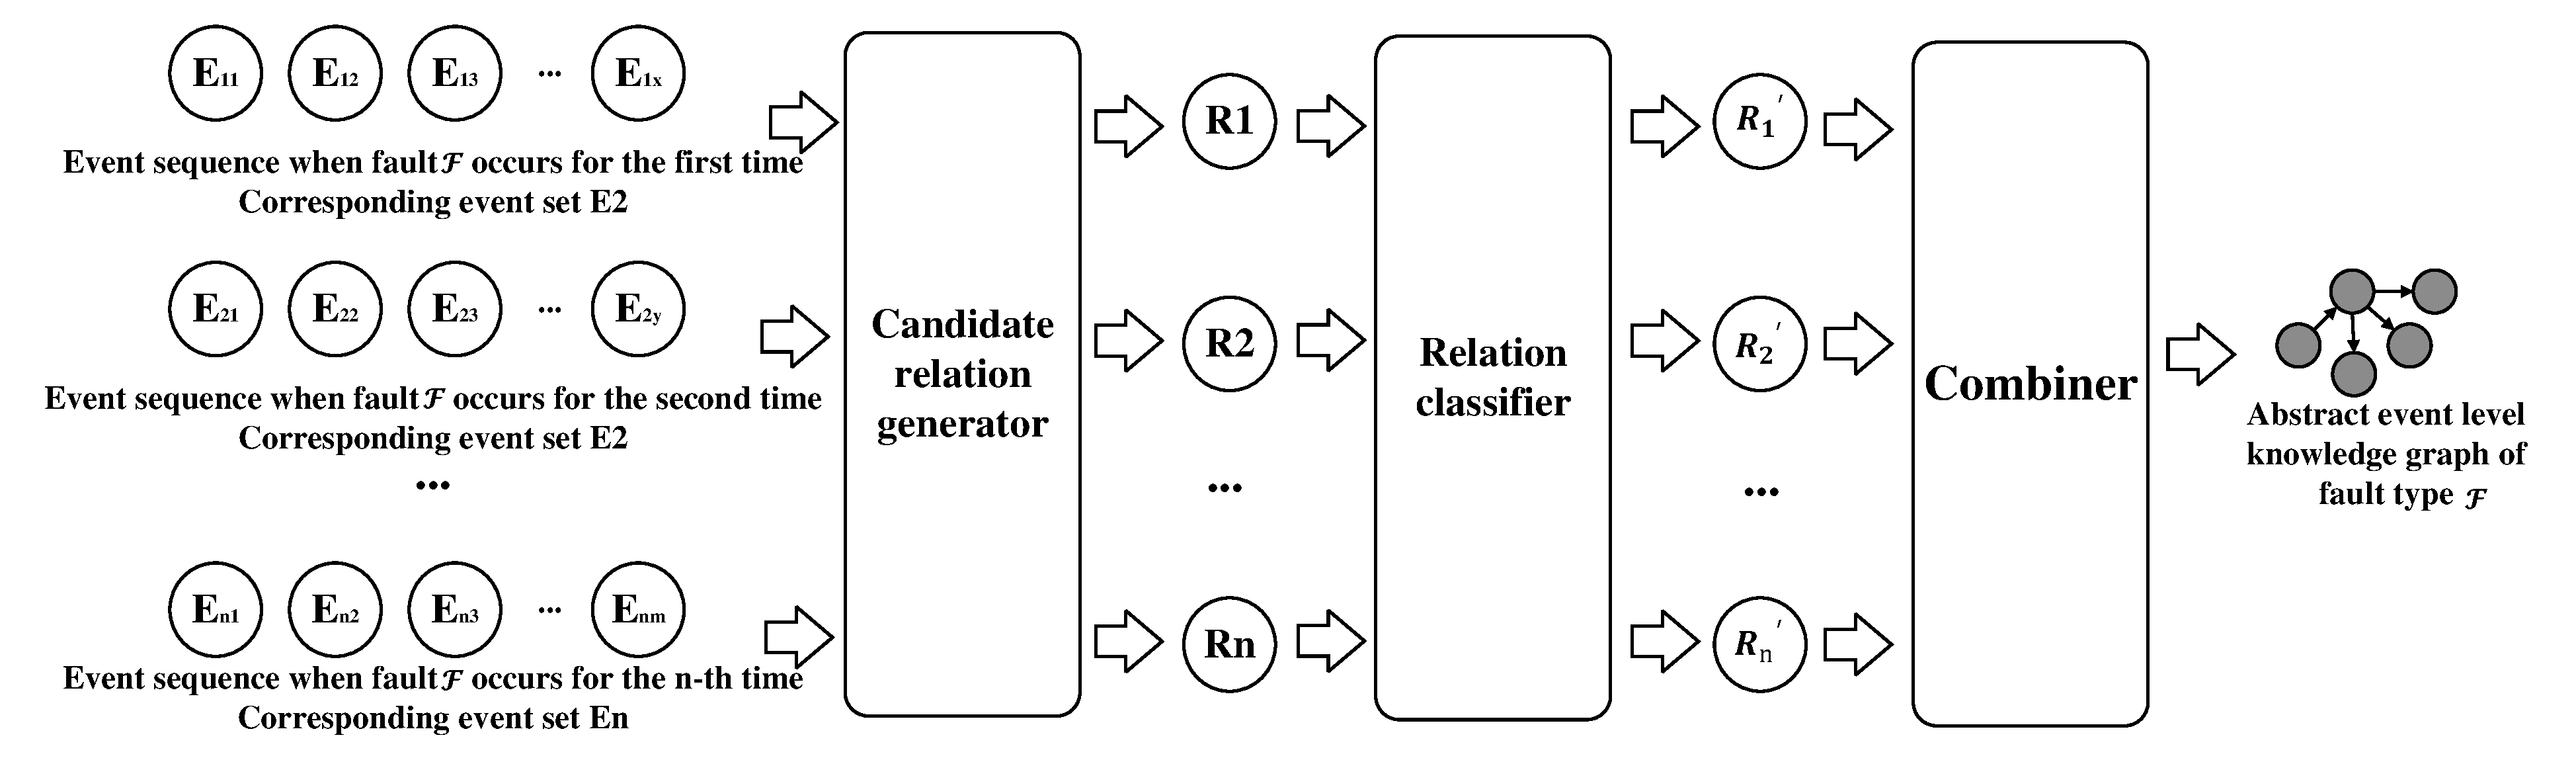
\includegraphics[width=.9\textwidth]{relation-combine.pdf}
    \caption{对应故障类型$\mathcal{F}$的组件-事件知识图谱生成流程\label{relation-combine}}
\end{figure}

图\ref{relation-combine}是故障类型$\mathcal{F}$对应的抽象事件层知识图谱构建流程示意图。图中构建流程可以使用算法\ref{construct-alg}表示。  
\begin{algorithm}[htbp]
	\renewcommand{\algorithmicrequire}{\textbf{输入:}}
	\renewcommand{\algorithmicensure}{\textbf{输出:}}
	\caption{组件-事件知识图谱构建算法}
	\label{construct-alg}
	\begin{algorithmic}[1]
		\REQUIRE 故障类型$\mathcal{F}$发生$n$次分别对应的事件集合$E_1,E_2,…,E_n$,分别对应的组件拓扑图$D_1,D_2,…,D_n$
		\ENSURE 故障类型$\mathcal{F}$对应的组件-事件知识图谱${kg}_{\mathcal{F}}$
		\STATE $i \gets 0$
		\WHILE {$i<n$}
            \STATE $R_{i} \gets$ 生成候选关系集合$(E_{i})$
            \STATE ${\mathbf{R}_\mathbf{i}}^\prime \gets$ 事件因果关系判别模型$(R_{i})$
        \ENDWHILE 
        \STATE $\mathcal{E}_{cause}=\ {\mathbf{R}_\mathbf{1}}^\prime\cup{\mathbf{R}_\mathbf{2}}^\prime\cup\ldots\cup{\mathbf{R}_\mathbf{n}}^\prime$
        \STATE $\mathcal{D}_{graph}= D_1 \cup D_2\cup \ldots \cup D_n$
        \STATE $\mathcal{E}_{graph} = Combiner(\mathcal{E}_{cause})$
        \STATE ${kg}_{\mathcal{F}} \gets link(\mathcal{D}_{graph}, \mathcal{E}_{graph})$
		\STATE \textbf{return} ${kg}_{\mathcal{F}}$
	\end{algorithmic}  
\end{algorithm}

具体上,故障类型$\mathcal{F}$对应组件-事件知识图谱的构建步骤描述如下:
% [itemsep= 15 pt,topsep = 20 pt,parsep =0pt,partopsep=0pt]
% \begin{itemize}[itemsep=0 pt,topsep = 0 pt,parsep =0pt,partopsep=0pt]
%     \item [(1)] 
%     生成候选关系集合:获取故障类型$\mathcal{F}$发生$n$次$\mathcal{F}_1,\mathcal{F}_2,…,\mathcal{F}_n$分别对应时间段内的事件集合$E_1,E_2,…,E_n$。针对每个时间段内的事件集合,首先基于TFIDF\cite{joachims1996probabilistic}和DTW算法\cite{mueen2016extracting}筛去部分噪声事件后将事件按时间顺序前后相连,得到候选关系集合$R_1,R_2,…,R_n$。  
%     \item [(2)]
%     生成因果关系集合:对候选关系集合$R_1,R_2,…,R_n$分别使用训练好的关系分类器判别该集合中每条候选关系是否为因果关系,仅保留判别为“存在”的因果关系,得到对应关系集合${\mathbf{R}_\mathbf{1}}^\prime$、${\mathbf{R}_\mathbf{2}}^\prime$、…、${\mathbf{R}_\mathbf{n}}^\prime$。
%     \item [(3)]
%     规约生成抽象事件因果拓扑:对分类器保留后的关系集合${\mathbf{R}_\mathbf{1}}^\prime$、${\mathbf{R}_\mathbf{2}}^\prime$、…、${\mathbf{R}_\mathbf{n}}^\prime$取并集,融合$\mathcal{F}$故障类型各个时间段内的事件因果关系对,其中每个事件都会按照类型归约到抽象事件,从而获得$\mathcal{F}$故障的抽象事件因果关系集合$\mathcal{E}_{cause}=\ {\mathbf{R}_\mathbf{1}}^\prime\cup{\mathbf{R}_\mathbf{2}}^\prime\cup\ldots\cup{\mathbf{R}_\mathbf{n}}^\prime$。
%     \item [(4)]
%     规约生成组件层拓扑:由于在相同应用上触发的故障,其组件层有着相同的拓扑逻辑结构。只需要将每个故障时间段组件图整合起来即可,具体整合方式为把具体id去除,只保留组件类型。如位于两个时间段的“ts-voucher-mysql-75945d946-x6hwl”和“ts-voucher-mysql-5sdf45sdd-xz45z”可以归约到组件实体“ts-voucher-mysql”。此外,针对“ts-voucher-mysql-75945d946-x6hwl”上发生“22:08:57/1575900537 找不到票务信息”这种组件到事件的关系,在组件-事件知识图谱中该关系会被存为“ts-voucher-mysql”上发生“找不到票务信息”。最后为了区分负载“ts-train-service”的Container,和负载“ts-ticketinfo-service”的Container,本文选择如文献\parencite{qiu2020causality-mining-knowledge-graph}对同类型组件进行序号标注的方式,将上述两个Container分别标注为“container1”,“container2”。
%     \item [(5)]
%     生成故障类型$\mathcal{F}$对应的组件-事件知识图谱:融合生成的关系对集合$\mathcal{E}_{cause}$,得到对应的有向图即为故障类型$\mathcal{F}$对应的抽象事件层知识图谱。再将组件实体与抽象事件实体按产生关系进行连接,就可以得到故障类型$\mathcal{F}$对应的组件-事件知识图谱。
%   \end{itemize}

(1)生成候选关系集合:获取故障类型$\mathcal{F}$发生$n$次$\mathcal{F}_1,\mathcal{F}_2,…,\mathcal{F}_n$分别对应时间段内的事件集合$E_1,E_2,…,E_n$。针对每个时间段内的事件集合,首先基于TFIDF\cite{joachims1996probabilistic}和DTW算法\cite{mueen2016extracting}筛去部分噪声事件后将事件按时间顺序前后相连,得到候选关系集合$R_1,R_2,…,R_n$。  

(2)生成因果关系集合:对候选关系集合$R_1,R_2,…,R_n$分别使用训练好的关系分类器判别该集合中每条候选关系是否为因果关系,仅保留判别为“存在”的因果关系,得到对应关系集合${\mathbf{R}_\mathbf{1}}^\prime$、${\mathbf{R}_\mathbf{2}}^\prime$、…、${\mathbf{R}_\mathbf{n}}^\prime$。

(3)规约生成抽象事件因果拓扑:对分类器保留后的关系集合${\mathbf{R}_\mathbf{1}}^\prime$、${\mathbf{R}_\mathbf{2}}^\prime$、…、${\mathbf{R}_\mathbf{n}}^\prime$取并集,融合$\mathcal{F}$故障类型各个时间段内的事件因果关系对,其中每个事件都会按照类型归约到抽象事件,从而获得$\mathcal{F}$故障的抽象事件因果关系集合$\mathcal{E}_{cause}=\ {\mathbf{R}_\mathbf{1}}^\prime\cup{\mathbf{R}_\mathbf{2}}^\prime\cup\ldots\cup{\mathbf{R}_\mathbf{n}}^\prime$。

(4)规约生成组件层拓扑:由于在相同应用上触发的故障,其组件层有着相同的拓扑逻辑结构。只需要将每个故障时间段组件图整合起来即可,具体整合方式为把具体id去除,只保留组件类型。如位于两个时间段的“ts-voucher-mysql-75945d946-x6hwl”和“ts-voucher-mysql-5sdf45sdd-xz45z”可以归约到组件实体“ts-voucher-mysql”。此外,针对“ts-voucher-mysql-75945d946-x6hwl”上发生“22:08:57/1575900537 找不到票务信息”这种组件到事件的关系,在组件-事件知识图谱中该关系会被存为“ts-voucher-mysql”上发生“找不到票务信息”。最后为了区分负载“ts-train-service”的Container,和负载“ts-ticketinfo-service”的Container,本文选择如文献\parencite{qiu2020causality-mining-knowledge-graph}对同类型组件进行序号标注的方式,将上述两个Container分别标注为“container1”,“container2”。

(5)生成故障类型$\mathcal{F}$对应的组件-事件知识图谱:融合生成的关系对集合$\mathcal{E}_{cause}$,得到对应的有向图即为故障类型$\mathcal{F}$对应的抽象事件层知识图谱。再将组件实体与抽象事件实体按产生关系进行连接,就可以得到故障类型$\mathcal{F}$对应的组件-事件知识图谱。

图\ref{graph-example}是上述构建过程生成的故障类型“数据库不可用无法查票”对应的组件-事件知识图谱的一部分。该知识图谱中,组件部分清晰地展示了ts-train-sevice,ts-ticketinfo-service,ts-travel-service分别部署在3个Container容器上,而这些容器托付在多个Pod中。同样的,这些Pod被负载在2台云服务器ECS中,并且这些ECS又被一台负载均衡器SLB所调控。在抽象事件部分,抽象事件实体被因果关系连接构成了抽象事件图,该图沉淀了ts-travel-service发生HttpServerError Exception 500故障的触发链知识。另外,抽象事件部分与组件部分被happen关系连接,本质上描述了抽象事件在哪类组件上产生。

\begin{figure}[htbp]
    \centering
    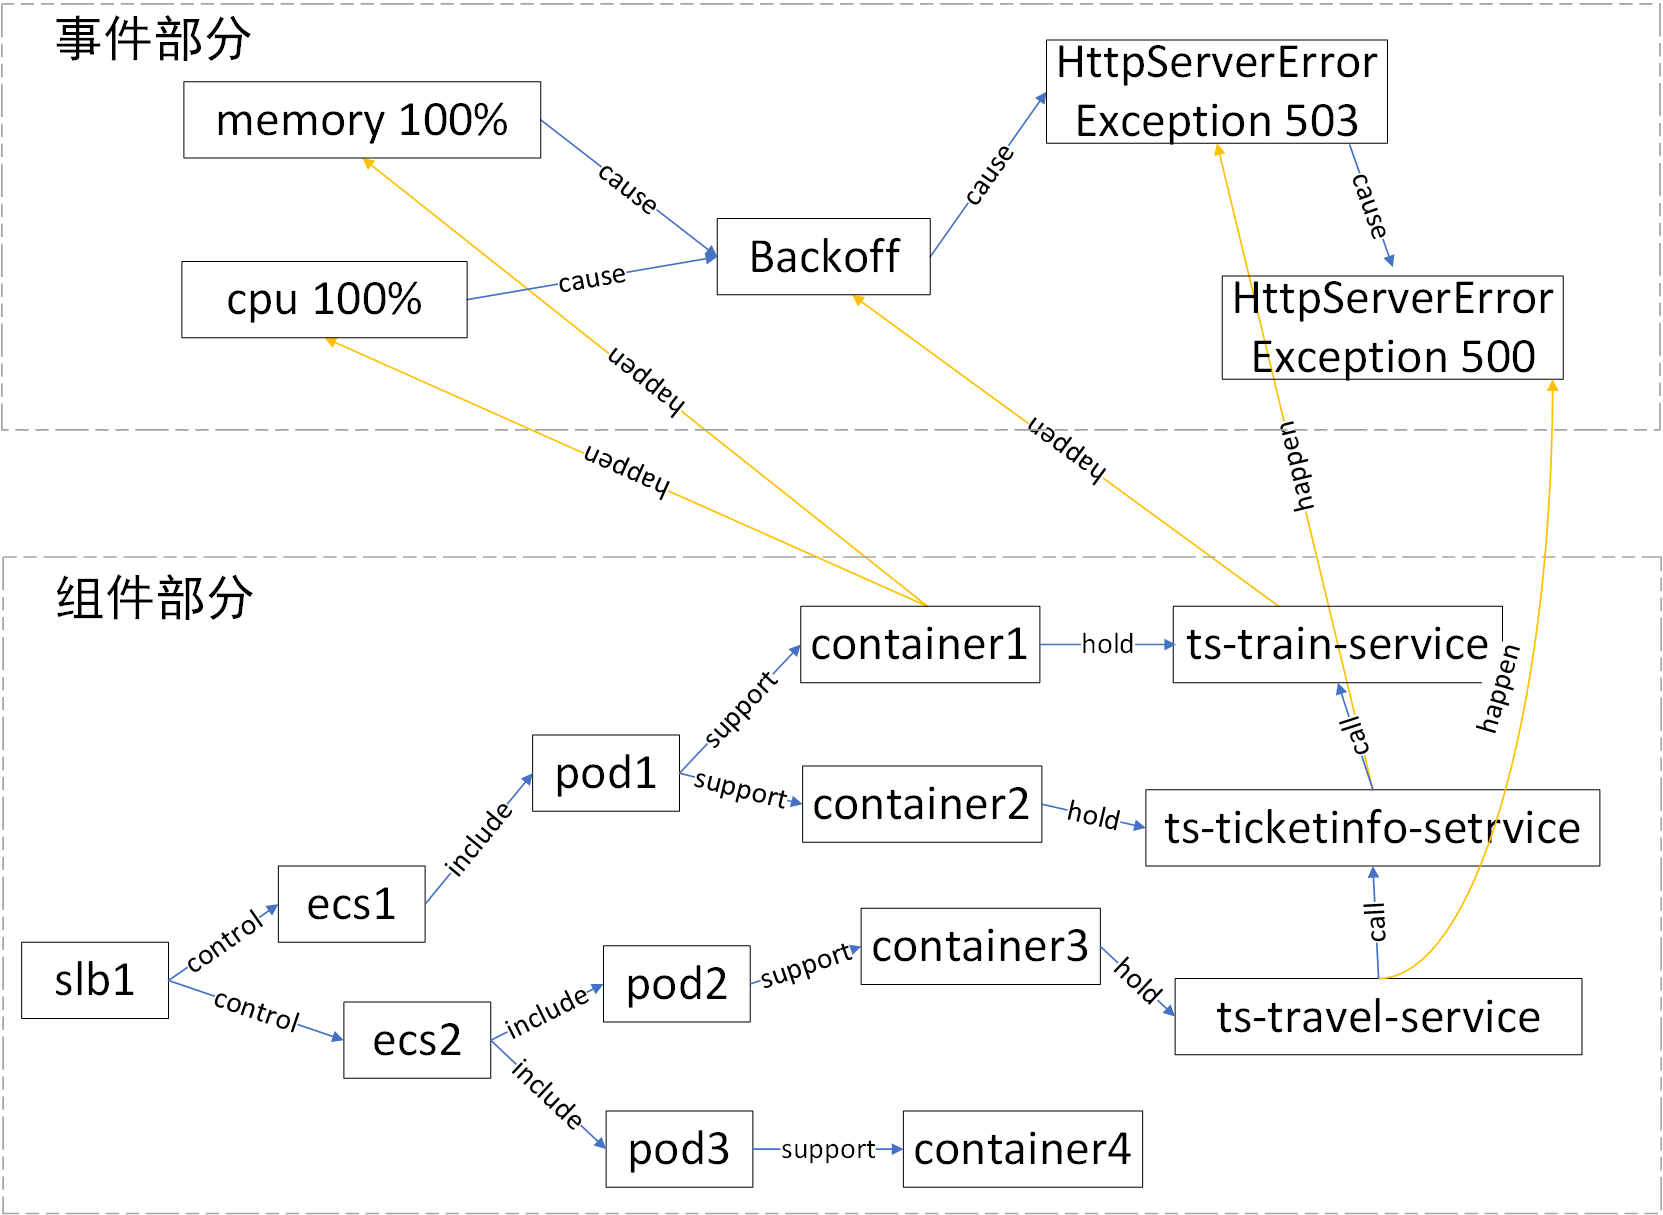
\includegraphics[width=.8\textwidth]{graph-example.png}
    \caption{数据库不可用无法查票故障对应知识图谱部分示例\label{graph-example}}
\end{figure}

% \newpage
\section{实验与分析}\label{event-cause-classidier-experiment}
由于组件间拓扑关系、组件到抽象事件的产生关系都可以准确获取,影响组件-事件知识图谱质量的只有事件间因果关系。因此,本节重点关注事件因果关系判别的效果,进行了相关实验的设计与实施。本节实验目的在于验证使用的6种事件特征,可以提升事件因果判别模型效果。本节共分为4小节介绍实验,包括数据集构建、评测指标、实验方法和实验结果分析。
\subsection{数据集构建}
%即\href{https://github.com/FudanSELab/train-ticket}{train-ticket}和\href{https://github.com/microservices-demo/microservices-demo}{sock-shop}。随后使用\href{https://github.com/asobti/kube-monkey}{kube-monkey}和\href{https://github.com/chaosblade-io/chaosblade}{ChaosBlade}
实验采用了阿里云kubernetes集群,集群各个组件数量如表\ref{component-num}所示。在该集群上部署了文献\parencite{zhou2018poster,rahman2019predicting}实验时分别使用的两个分布式应用,即train-ticket和sock-shop。随后使用kube-monkey和ChaosBlade向应用注入异常以模拟故障。在异常注入到故障产生的时间段中,阿里云的SLS平台负责收集实时产生的日志数据和指标时序数据。所模拟故障的数据统计信息如表\ref{failure-simulation-info}所示。这些数据后续经过事件生成模块,均转化为了事件类型数据。
\begin{table}[htbp]
    \caption{集群各类组件数量统计}
    \label{component-num}
    \centering
    \begin{tabular}{ccc}
    \toprule[1.5pt]
    组件名称      & train-ticket & sock-shop        \\ \midrule[1.5pt]
    VPC       & 34           & 28 \\
    SLB       & 30           & 36 \\
    ECS       & 30           & 30 \\
    Pod       & 215          & 181 \\
    Container & 720          & 621 \\
    Service   & 172          & 132 \\ \midrule[1pt]
    共计   & 1201          & 1028 \\ \bottomrule[1.5pt]
    \end{tabular}
\end{table}

本实验对数据集中的关系种类进行了标注,标注数据覆盖了每一种故障类型。其中对于每种故障类型,随机抽取了该类故障类型2个具体时间段的数据进行了标注,只对认为有因果关系的事件对标注为1,其余事件对默认无因果关系标注为0。
\begin{table}[htbp]
    \caption{故障模拟信息}
    \centering
    \label{failure-simulation-info}
    \begin{tabular}{ccc}
    \toprule[1.5pt]
    分布式应用       & train-ticket & \multicolumn{1}{c}{sock-shop} \\ \midrule[1.5pt]
    时间跨度       & 25天          & 14天                           \\
    平均故障时间段跨度  & 303s         & 310s                          \\
    单个故障时间段含有事件数目 & 4823         & 3352                          \\
    故障次数       & 491          & 573                           \\
    % 故障次数       & 423          & 550                           \\
    故障种类       & 10           & 17                            \\
    事件类型种类     & 204          & 211                           \\ 
    \bottomrule[1.5pt]
    \end{tabular}
\end{table}

由于事件因果判别模型是根据事件对统计特征发掘事件间因果关系,与事件来自何种应用无关,所以本块实验不区分事件来自于train-ticket还是sock-shop,直接把两个应用来源的标注事件对整合起来。最终标注为1的事件对共计286条,其余默认无关系的共计8,250,290‬条。数据集train-ticket、sock-shop的标注信息如下表\ref{event-cause-label}所示。由于正负样本数量级差距较大,后续选择了按照正负样本比1:10随机抽取了一批负样本数据用于训练。抽取出用于训练的数据共包含正样本286条,负样本2860条。
\newpage
\begin{table}[htbp]
    \caption{事件对因果关系标注数据集}
    \centering
    \label{event-cause-label}
    \begin{tabular}{cccc}
    \toprule[1.5pt]
        分布式应用     & 正例  & 负例      & 总计      \\ \midrule[1.5pt]
    train-ticket & 121 & 3610827 & 3610948 \\
    sock-shop    & 165 & 4639463 & 4639628 \\ \midrule[1pt]
    总计           & 286 & 8250290 & 8250576 \\ 
    \bottomrule[1.5pt]
    \end{tabular}
\end{table}

\subsection{评测指标}
由于事件因果关系判别模型目的在于正确判别事件对之间的关系,所以本块实验以被标注的事件对关系被识别的精确率($precision$)、召回率($recall$)和$F1$值作为评测标准。计算公式分别如式\ref{relation-classifier-p}、\ref{relation-classifier-r}和\ref{relation-classifier-f}所示。
% \begin{equation}
%     \begin{array}{c}
%     precision =\frac{\left|R_{correct }\right|}{|R_{predict}|} \\
%      recall =\frac{\left|R_{correct }\right|}{\left|R_{label }\right|}  \\
%     F 1=\frac{2 \times  precision  \times  recall }{precision + recall }
%     \end{array}
%     \label{relation-classifier-prf}
% \end{equation}{\Huge } 
\begin{equation}
    \centering
    precision =\frac{\left|R_{correct }\right|}{|R_{predict}|}
    \label{relation-classifier-p}
\end{equation}
\begin{equation}
    \centering
    recall =\frac{\left|R_{correct }\right|}{\left|R_{label }\right|}
    \label{relation-classifier-r}
\end{equation}
\begin{equation}
    \centering
    F 1=\frac{2 \times  precision  \times  recall }{precision + recall }
    \label{relation-classifier-f}
\end{equation}

其中,$\left|R_{\text {correct }}\right|$为同时被标注存在因果关系且被判别为存在因果关系的事件对数,$|R_{\text {predict}}|$为模型判别为有因果关系的事件对数,$\left|R_{\text {label }}\right|$为被标注存在因果关系的事件对数。

\subsection{实验方法}
\begin{table}[htbp]
    \caption{对比特征集}
    \centering
    \label{only-prob-feature}
    \begin{tabular}{cc}
    \toprule[1.5pt]
    特征名    & 计算方式                  \\ \midrule[1.5pt]
    共现次数\cite{liu1998integrating}   & A,B共现次数               \\
    关系置信度\cite{liu1998integrating}  & $P(B|A)$                \\
    逆关系置信度\cite{liu1998integrating} & $P(A|B)$                \\
    Lift\cite{liu1998integrating}  & $P(AB)/((P(A) \cdot P(B)))$ \\
    KULC\cite{liu1998integrating}   & $(P(A|B) + P(B|A))/2$   \\
    IR\cite{liu1998integrating}    & $P(A)/(B)$              \\ 
    Pearson\cite{mahimkar2008troubleshooting} & 皮尔逊相关系数         \\
    Location\cite{nie2016mining-causality-graph}  & 事件是否发生在同一个设备 \\ 
    \bottomrule[1.5pt]
    \end{tabular}
\end{table}
对于标注数据中的正样本286条、负样本2860条,随机抽取平分为5份,以便采用5折交叉验证方法。其中每份数据集中包含正样本数57,负样本数572。
% 根据文献\parencite{nie2016mining-causality-graph,qiu2020causality-mining-knowledge-graph}中的实验,
本块实验选用了SVM、XGBoost、随机森林、逻辑回归和多层感知机共计五种经典模型进行了对比实验,以选出最优表现的分类模型。

另外,为了验证本文选用的6种事件特征对因果关系判别的提升(其中只有“关系置信度”为基于概率的特征),实验总结了已有工作中使用的特征进行对比(其中前 6 项均是基于概率的特征),如表\ref{only-prob-feature}所示。随后,用“multi”表示本文使用的事件特征集,“base”表示对比特征集。


% \begin{table}[htbp]
%     \caption{本文选用特征}
%     \label{this-paper-use}
%     \begin{tabular}{cc}
%     \toprule[1.5pt]
%     特征名     & 含义            \\ \midrule[1.5pt]
%     皮尔逊相关系数 & 事件发生频次变化的相关性  \\
%     关系置信度   & 两事件发生的条件概率    \\
%     发生距离    & 事件发生所在设备的距离度量 \\
%     平均时间差   & 事件发生的前后时间差均值  \\
%     周期性     & 事件发生周期性度量     \\
%     关键性度量   & 事件与故障发生关联度    \\ 
%     \bottomrule[1.5pt]
%     \end{tabular}
% \end{table}
\subsection{实验结果与分析}

实验统计了各个模型在进行5折交叉验证时,所计算得到的精确率、召回率和F1值,结果统计如表\ref{cause-relation-result}所示。对于每个模型,都尝试了多种超参数组合,最终通过网格搜索选择可使其达到最佳效果的超参数组合。

\begin{table}[htbp]
    \caption{各分类模型事件因果关系判别结果}
    \centering
    \label{cause-relation-result}
    \begin{tabular}{ccccc}
    \toprule[1.5pt]
    模型      & 选用数据特征              & 精确率            & 召回率                           & F1             \\ \midrule[1.5pt]
    SVM     & multi               & \textbf{0.951} & 0.961                         & \textbf{0.956} \\
    XGBoost & multi               & 0.911          & 0.895                         & 0.903          \\
    随机森林    & multi               & 0.950          & 0.792                         & 0.864          \\
    逻辑回归    & multi               & 0.913          & 0.845                         & 0.878          \\
    多层感知机   & multi               & 0.892          & \textbf{1.0}                  & 0.943          \\ \midrule[1pt]
    SVM     & base & 0.822          & 0.769                         & 0.795          \\
    XGBoost & base & 0.779          & 0.756                         & 0.767          \\
    随机森林    & base & 0.831          & 0.770                         & 0.799          \\
    逻辑回归    & base & 0.782          & 0.754                         & 0.768          \\
    多层感知机   & base & 0.739          & 0.816  & 0.776          \\ \bottomrule[1.5pt]
    \end{tabular}
\end{table}

在表\ref{cause-relation-result}统计的结果中,SVM模型的精确率、召回率和F1值均达到了0.95以上,而随机森林、逻辑回归和XGBoost效果较差。多层感知机召回率达到了1.0,但精确率只有0.892,可见其偏向于将数据都判别为正例,判别结果会出现过多的假阳。在本实验中,SVM模型取得最佳效果时所设置的超参数组合为高斯核函数、$sigma=1$、松弛变量=5。另外,对比选用的数据特征,发现使用“multi”比只使用“base”的特征在所有模型上都取得了更好的效果,证明了本文设计并引入新的事件特征对因果关系判别效果有显著提升。

\section{本章小结}
本章主要介绍了组件-事件知识图谱的构建方式,该图谱整合了所有种类的数据。对于组件部分数据,云服务商会提供开放的API返回分布式集群含有的组件属性信息、组件数量及每个组件间的关联关系,微服务访问追踪系统可以获取微服务间访问拓扑关系。在事件数据层面,通过聚类、异常检测算法和模板匹配将多源异构数据统一为了事件类型数据,随后训练关系分类器挖掘事件间因果关系,最后将历史数据按照故障类型分组再沉淀生成对应故障类型的组件-事件知识图谱。在实验部分,实验结果验证了本文新设计引入的事件特征,对事件因果关系判别的有效性。下一章会在此基础上,研究组件-事件知识图谱的表示学习工作。

% 知识图谱可以用资源描述框架(RDF)\cite{heim2009relfinder}来表示,它包含一个主语、谓语和宾语,如等式\ref{rdf}所示。RDF由节点和边组成。节点表示实体和属性,边表示实体和实体之间的关系以及实体和属性之间的关系。
% \begin{equation}
%     Subject \stackrel{predicate}{\longrightarrow} Object
%     \label{rdf}
% \end{equation}

% 定义2:抽象事件。抽象事件是同类型事件规约后的形式。只包含包括3个部分:
% TypeId:抽象事件唯一标识;
% LocationType:抽象事件发生在何种组件上;
% Event type:抽象事件类型名;
% 定义3:事件知识图谱。事件知识图谱是三元组集合(抽象事件e_1,r,抽象事件e_2),其中r为因果关系。

\chapter{组件-事件知识图谱表示学习}\label{chapter-3}
在已有的知识库中(如FB15K\cite{bordes2013translatingE}和YAGO37\cite{guo2018knowledge}),由于每个三元组$\left(head, relation, tail\right)$都可以视作一条知识而单独存在,知识图谱可以用多个三元组组成的集合表示,即 $\mathcal{KG}=\left\{\left(e_{i}, r_{k}, e_{j}\right)\right\}$(其中$i$、$j$为实体索引,$k$为关系索引)。因此,已有的大多数知识表示模型都是输入三元组$\left(head, relation, tail\right)$,然后着重于缩短这三者嵌入表示之间的语义距离。

在本文的组件-事件知识图谱$G=(\mathcal{F}, \mathcal{V}, \mathcal{E}, \mathcal{R})$中,每个组件-事件知识图谱都对应着一个故障类型$\mathcal{F}$,这使得每个三元组的成立与其上下文背景信息有关,且每个实体在不同的上下文中应有不同的嵌入表示,即应随着上下文的变化而动态地表示。详细分析如章节\ref{backgroud-analysis}所示。

虽然文献\parencite{feng2016gake,shi2017knowledge}尝试将图结构上下文引入嵌入表示,但是它们都将原本的图结构转为邻居上下文、路径上下文再进行嵌入表示学习。这种方式不足以获取全面的图结构上下文信息,且不能满足动态的嵌入表示学习,即不能根据具体上下文给同一实体不同的嵌入表示。
% 所以本文利用图神经网络获取组件-事件知识图谱中的上下文结构信息,再结合实体的语义信息,获取动态的实体嵌入表示。

为了满足实体随上下文动态表示,本章设计了针对组件-事件知识图谱的知识表示学习方案(Dynamic Knowledge Graph Embedding,DKGE)。本章共分为4节展开介绍:首先,本章介绍了所提表示学习方案的总体框架;随后,本章进行了场景分析,罗列了组件-事件知识图谱进行表示学习时要解决的问题;然后详细介绍了针对组件-事件知识图谱的表示学习模型;最后,本章设计了详细的实验验证本文模型的有效性。
\section{总体框架}
本章提出的针对组件-事件知识图谱的表示学习方案的总体框架图如\ref{kg-repre-total}所示。由图可见,输入为三元组及其对应的上下文图结构。实体表示被分为了语义表示和结构表示两部分,语义表示通过实体文本属性训练的预训练模型获取,结构表示通过引入注意力机制的关系图卷积网络获取。关系表示则只有语义表示。整个表示学习模型,通过训练模块计算损失函数并更新模型参数,通过预测模块检测其效果。
\begin{figure}[htbp]
    \centering
    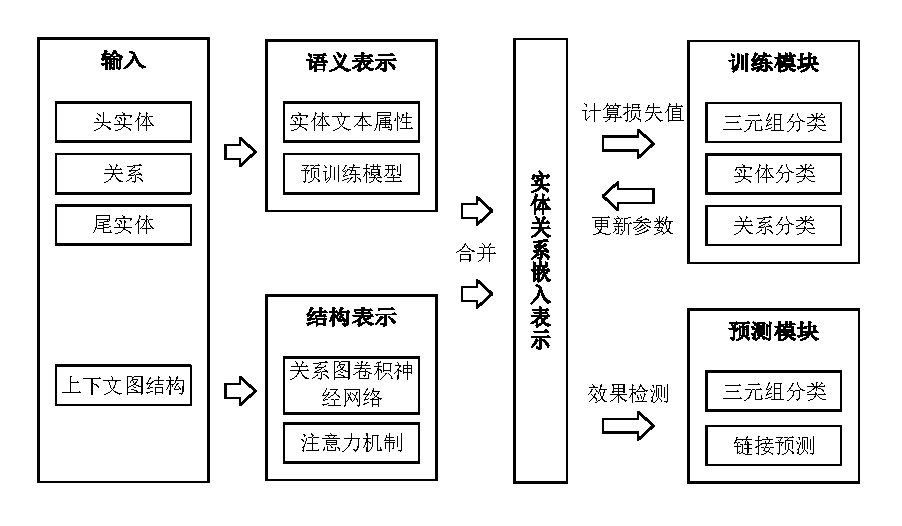
\includegraphics[width=.75\textwidth]{kg-repre-total.pdf}
    \caption{组件-事件知识图谱动态表示学习总体框架图\label{kg-repre-total}}
\end{figure}

\section{场景分析}\label{backgroud-analysis}
% GCN  RGCN  SACN KBAT
本节主要分析了组件-事件知识图谱的特性,解释了为何本文的知识表示学习与上下文背景信息相关,且需要动态的嵌入表示。

\subsection{上下文背景信息}\label{context-analysis}
在组件-事件知识图谱中,一个三元组的成立与其上下文拓扑关系有关,这使得一个三元组不能被视为一条可以单独存在的知识。下面是以图\ref{graph-example}中信息为例,对组件-事件知识图谱中三大类关系的分析:

(1)抽象事件间的因果关系。以三元组$\left(Backoff, cause, HttpServerError Exception 503\right)$为例,该三元组中$Backoff$(微服务重启失败)和$HttpServerError 503$(微服务服务不可用)之间不一定有触发关系。该三元组的成立,需要一定的背景信息如式\ref{event-event-relation}所示。
% ,即需要这两个事件发生在同一个微服务组件、或者有交互依赖关系的两个微服务组件。
\begin{equation}
    \begin{aligned}
        &\left ( ts-train-service, happen, Backoff \right ) \\
        &\wedge \left ( ts-ticketinfo-service, happen, HttpServerError Exception 503 \right ) \\
        &\wedge \left ( ts-ticketinfo-service, call, ts-train-service \right ) \\
        &\Rightarrow \left ( Backoff, \boldsymbol{cause}, HttpServerError Exception 503 \right )
    \end{aligned}
\label{event-event-relation}
\end{equation}

% 1)事件到事件的因果关系。以预测三元组中尾实体$\left(Backoff, cause, \textcolor[rgb]{1,0,0}{?}\right)$为例,推理关系如式\ref{event-event-relation-entity}所示,即需要这两个事件发生在同一个微服务组件、或者有交互关系的两个微服务组件。
% \begin{equation}
%     \begin{aligned}
%         &\left ( ts-train-service, happen, Backoff \right ) \\
%         &\wedge \left ( ts-ticketinfo-service, happen, HttpServerError Exception 503 \right ) \\
%         &\wedge \left ( ts-ticketinfo-service, call, ts-train-service \right ) \\
%         &\Rightarrow \left ( Backoff, \boldsymbol{cause}, HttpServerError Exception 503 \right )
%     \end{aligned}
% \label{event-event-relation-entity}
% \end{equation}

(2)组件到抽象事件的发生关系。以三元组$(ts-travel-service, happen, HttpServerError Exception 500)$为例,该三元组中$ts-travel-service$是否会发生事件$HttpServerError$$Exception 500$同样与其周边设备的状态有关。该三元组成立依据于式\ref{event-device-relation}中所示的条件。
\begin{equation}
    \begin{aligned}
        &\left ( ts-ticketinfo-service, happen,  HttpServerError Exception 503\right ) \\
        &\wedge \left ( ts-travel-service, call, ts-ticketinfo-service \right ) \\
        &\wedge \left ( HttpServerError Exception 503, cause, HttpServerError Exception 500 \right ) \\
        &\Rightarrow \left ( ts-travel-service, \boldsymbol{happen}, HttpServerError Exception 500 \right )
    \end{aligned}
\label{event-device-relation}
\end{equation}

(3)组件到组件的交互关系。以三元组$\left( container1, hold, ts-train-service \right)$为例,该三元组中$container1$负载着$ts-train-service$而不是其他微服务,同样需要借助背景信息才能推导出来。背景信息推导出该三元组成立的过程,如式\ref{device-device-relation}所示。
\begin{equation}
    \begin{aligned}
        &\left ( container1, happen,  cpu 100\% \right ) \\
        &\wedge \left ( container1, happen,  memory 100\% \right) \\
        &\wedge \left ( ts-train-service, happen,  Backoff \right) \\
        &\wedge \left ( cpu 100\%, cause,  Backoff \right) \\
        &\wedge \left ( memory 100\%, cause,  Backoff \right) \\
        &\Rightarrow \left ( container1, \boldsymbol{hold}, ts-train-service \right )
    \end{aligned}
\label{device-device-relation}
\end{equation}

由上述分析可见,组件-事件知识图谱中每条三元组都不能作为一条知识单独存在,而是知识图谱中三元组之间相互佐证使得整个拓扑图成为了蕴含知识的知识图谱。由此启发,组件-事件知识图谱的知识表示学习需要将实体所在上下文背景信息考虑进去,才能学习得到有效的实体与关系嵌入表示。
% 在组件-事件知识图谱表示学习中,需要考虑三元组的上下文。
% 已有的方式
% 引入逻辑规则,在传统的知识图谱中,关系都有丰富的语义信息(与常识知识有关),可以根据语义信息生成一些推理规则。比如
% isMarriedTo(x,y)->isMarriedTo(y,x)
% hasChild(x,y)且isCitizenOf(y,z)->isCitizenOd(x,z)
% playsFor(x,y)->isAffiliatedTo(x,y)
% 在组件-事件知识图谱中,只有因果关系,产生关系和交互关系,语义信息不足,生成的规则不具有通用性。规则是否成立其与具体的拓扑关系、抽象事件类型、组件类型都有关系。比如\ref{graph-example}中从“微服务ts-train-service发生BackOff就会导致请求它的微服务ts-ticketinfo-service发生HttpServerError”可以生成规则“微服务x发生BackOff就会导致请求它的微服务y发生HttpServerError”。该条规则只在当前的分布式应用可用,随着应用更新(添加了备用的微服务ts-train-service2或者开发人员添加异常处理使之不报错)或在其他的两个有访问关系的微服务之间,该条规则就会不适用。一方面规则需要大量人工编写审核,一方面即使自动生成规则也没有通用性,所以引入规则进行知识表示学习不可行。
\subsection{动态嵌入表示}
根据\ref{context-analysis}节分析,本文知识图谱表示学习需要引入上下文背景信息。在引入上下文背景信息方面,文献\parencite{feng2016gake,shi2017knowledge}将实体所在的图结构转为邻居上下文、路径上下文,通过最大化实体在其上下文的条件概率进行嵌入表示学习。但这种最大化概率的方式,对实体、关系的嵌入表示是静态的,即一旦训练完成嵌入表示是不会再随着上下文改变的。

这种获取静态嵌入表示的方法不适用于组件-事件知识图谱的表示学习。因为同一抽象事件由于其所在上下文不同、所在设备不同应当有着不同的嵌入表示。如图\ref{order-service-error}所示是"订票服务不可用"故障对应的组件-事件知识图谱部分示意图,在该图中同样存在$Backoff$抽象事件和$\left(ts-travel-service, happen, HttpServiceError Exception 500\right)$三元组,但该图中$ts-travel-service$发生$HttpServiceError Exception 500$是由于订票微服务$ts-order-service$上发生的抽象事件$Backoff$导致的。相对应的图\ref{graph-example}中$ts-travel-service$发生$HttpServiceError Exception 500$是微服务$ts-train-service$上的$Backoff$间接导致的,对应着"数据库不可用无法查票"故障。在这两个故障场景中,抽象事件$HttpServiceError Exception 500$是由不同原因导致的,所以应有不同的嵌入表示。抽象事件$Backoff$发生在不同的微服务上,也应有着不同的嵌入表示。所以,在组件-事件知识图谱中,实体嵌入表示需要随上下文信息动态变化。
\begin{figure}[htbp]
    \centering
    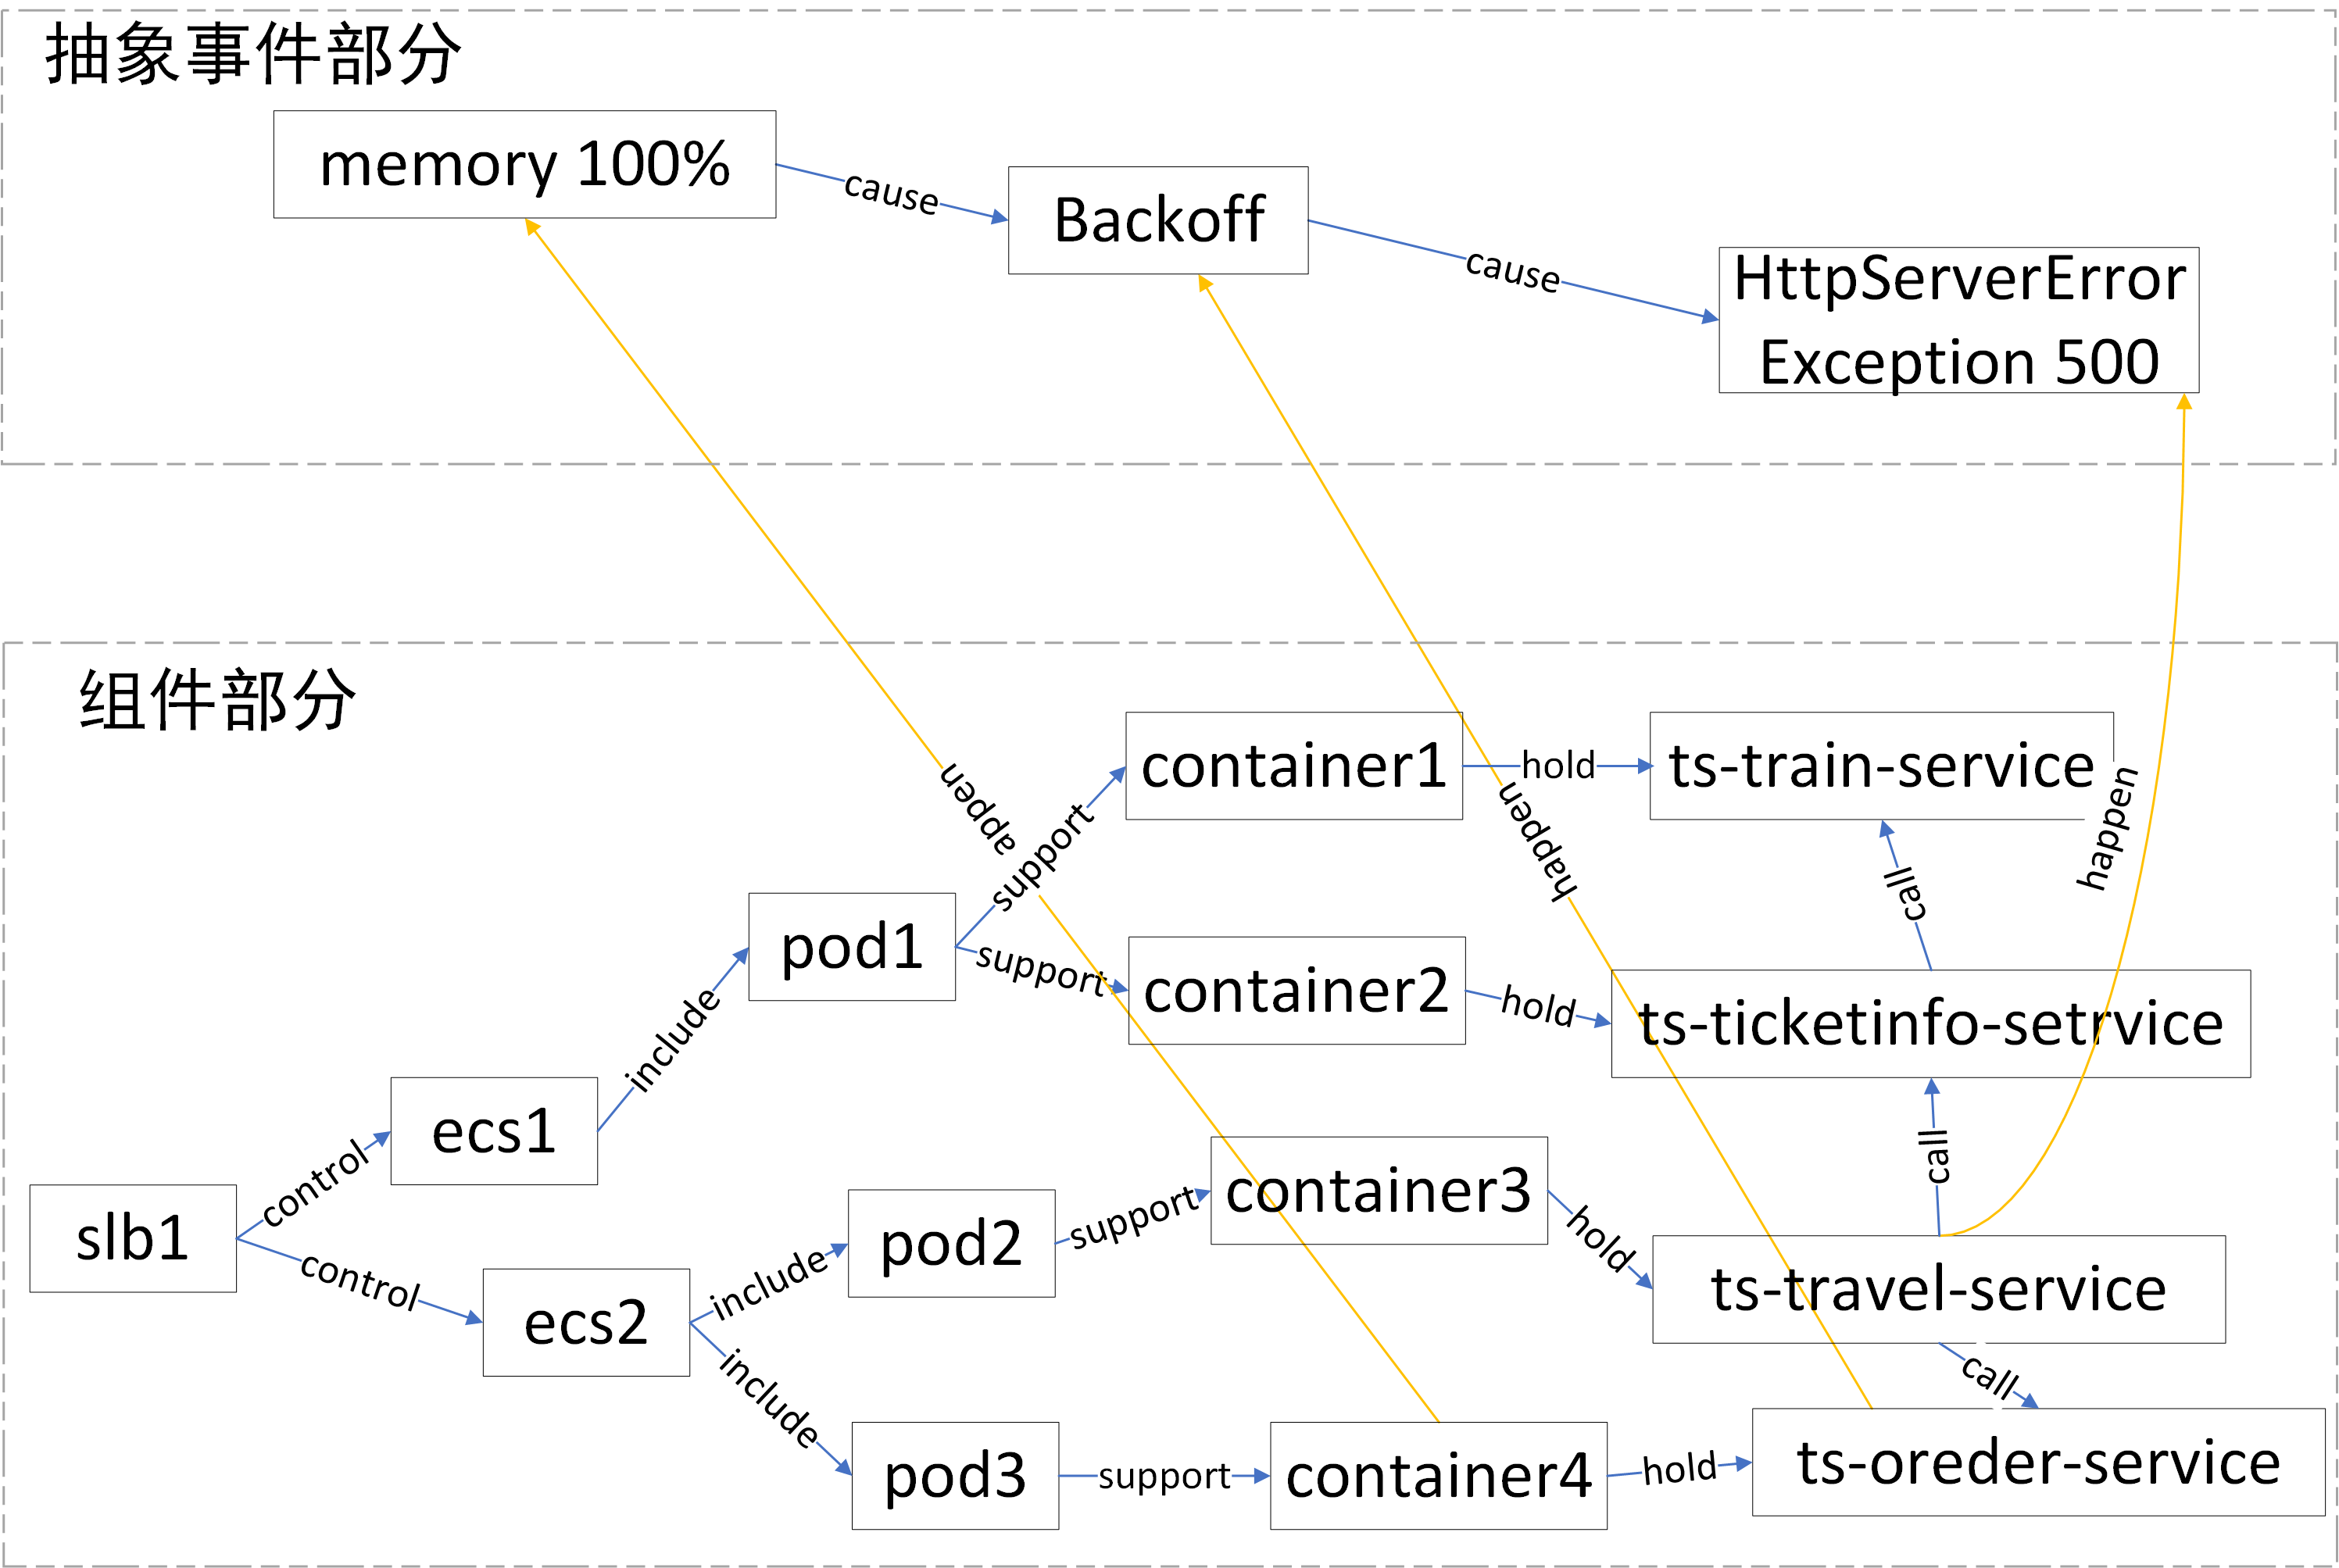
\includegraphics[width=.7\textwidth]{order-service-error.png}
    \caption{订票服务不可用故障对应知识图谱部分示例\label{order-service-error}}
\end{figure}

根据上下文进行动态表示在词嵌入领域已经有大量的相关工作。在最初的工作中,word2vec\cite{mikolov2013efficient}最大化单词在上下文出现的概率,将每个单词表示为低维稠密的静态向量,却忽视了单词在不同上下文含义不同。为了识别单词在不同上下文中具体的语义,ELMo\cite{peters2018deep}提出使用双层记忆网络,Bert\cite{devlin2018bert}使用基于自注意力机制的Transformer\cite{vaswani2017attention}编码层以获取单词随上下文变动的动态词向量。其中Bert所使用的Transformer结构其实是将一段文本看做单词为结点的全连接图。

受此启发,本文可以将知识图谱看作稀疏有向图,使用关系图卷积神经网络作为编码器,获取实体的上下文图结构信息。
% 1.rgcn后面连接的解码器什么样子
% 2.loss函数怎么计算 分类 关系 还是 头尾实体预测
% 3.模型的输入是什么

\section{组件-事件知识图谱动态表示学习模型}
上文介绍到实体会出现在不同的上下文中,所以需要随着上下文的变化拥有动态的向量表示。由于RGCN可以充分提取图的拓扑结构信息,所以本文使用RGCN作为编码器,获取实体的上下文图结构信息。在RGCN部分,为了让实体对不同的邻居结点有不同的侧重,本文又引入了注意力机制给邻居结点赋予了不同的权重,即Attention-RGCN。

本节详细介绍了针对组件-事件知识图谱的表示学习方法,分为模型结构、模型训练和预测3小节。
\subsection{模型结构}
整个模型结构如图\ref{kg-representation}所示,可见主要包括嵌入层、Attention-RGCN层、三元组分类层、实体分类层和关系分类层。下面将会分别对每一层展开介绍。
\begin{figure}[htbp]
    \centering
    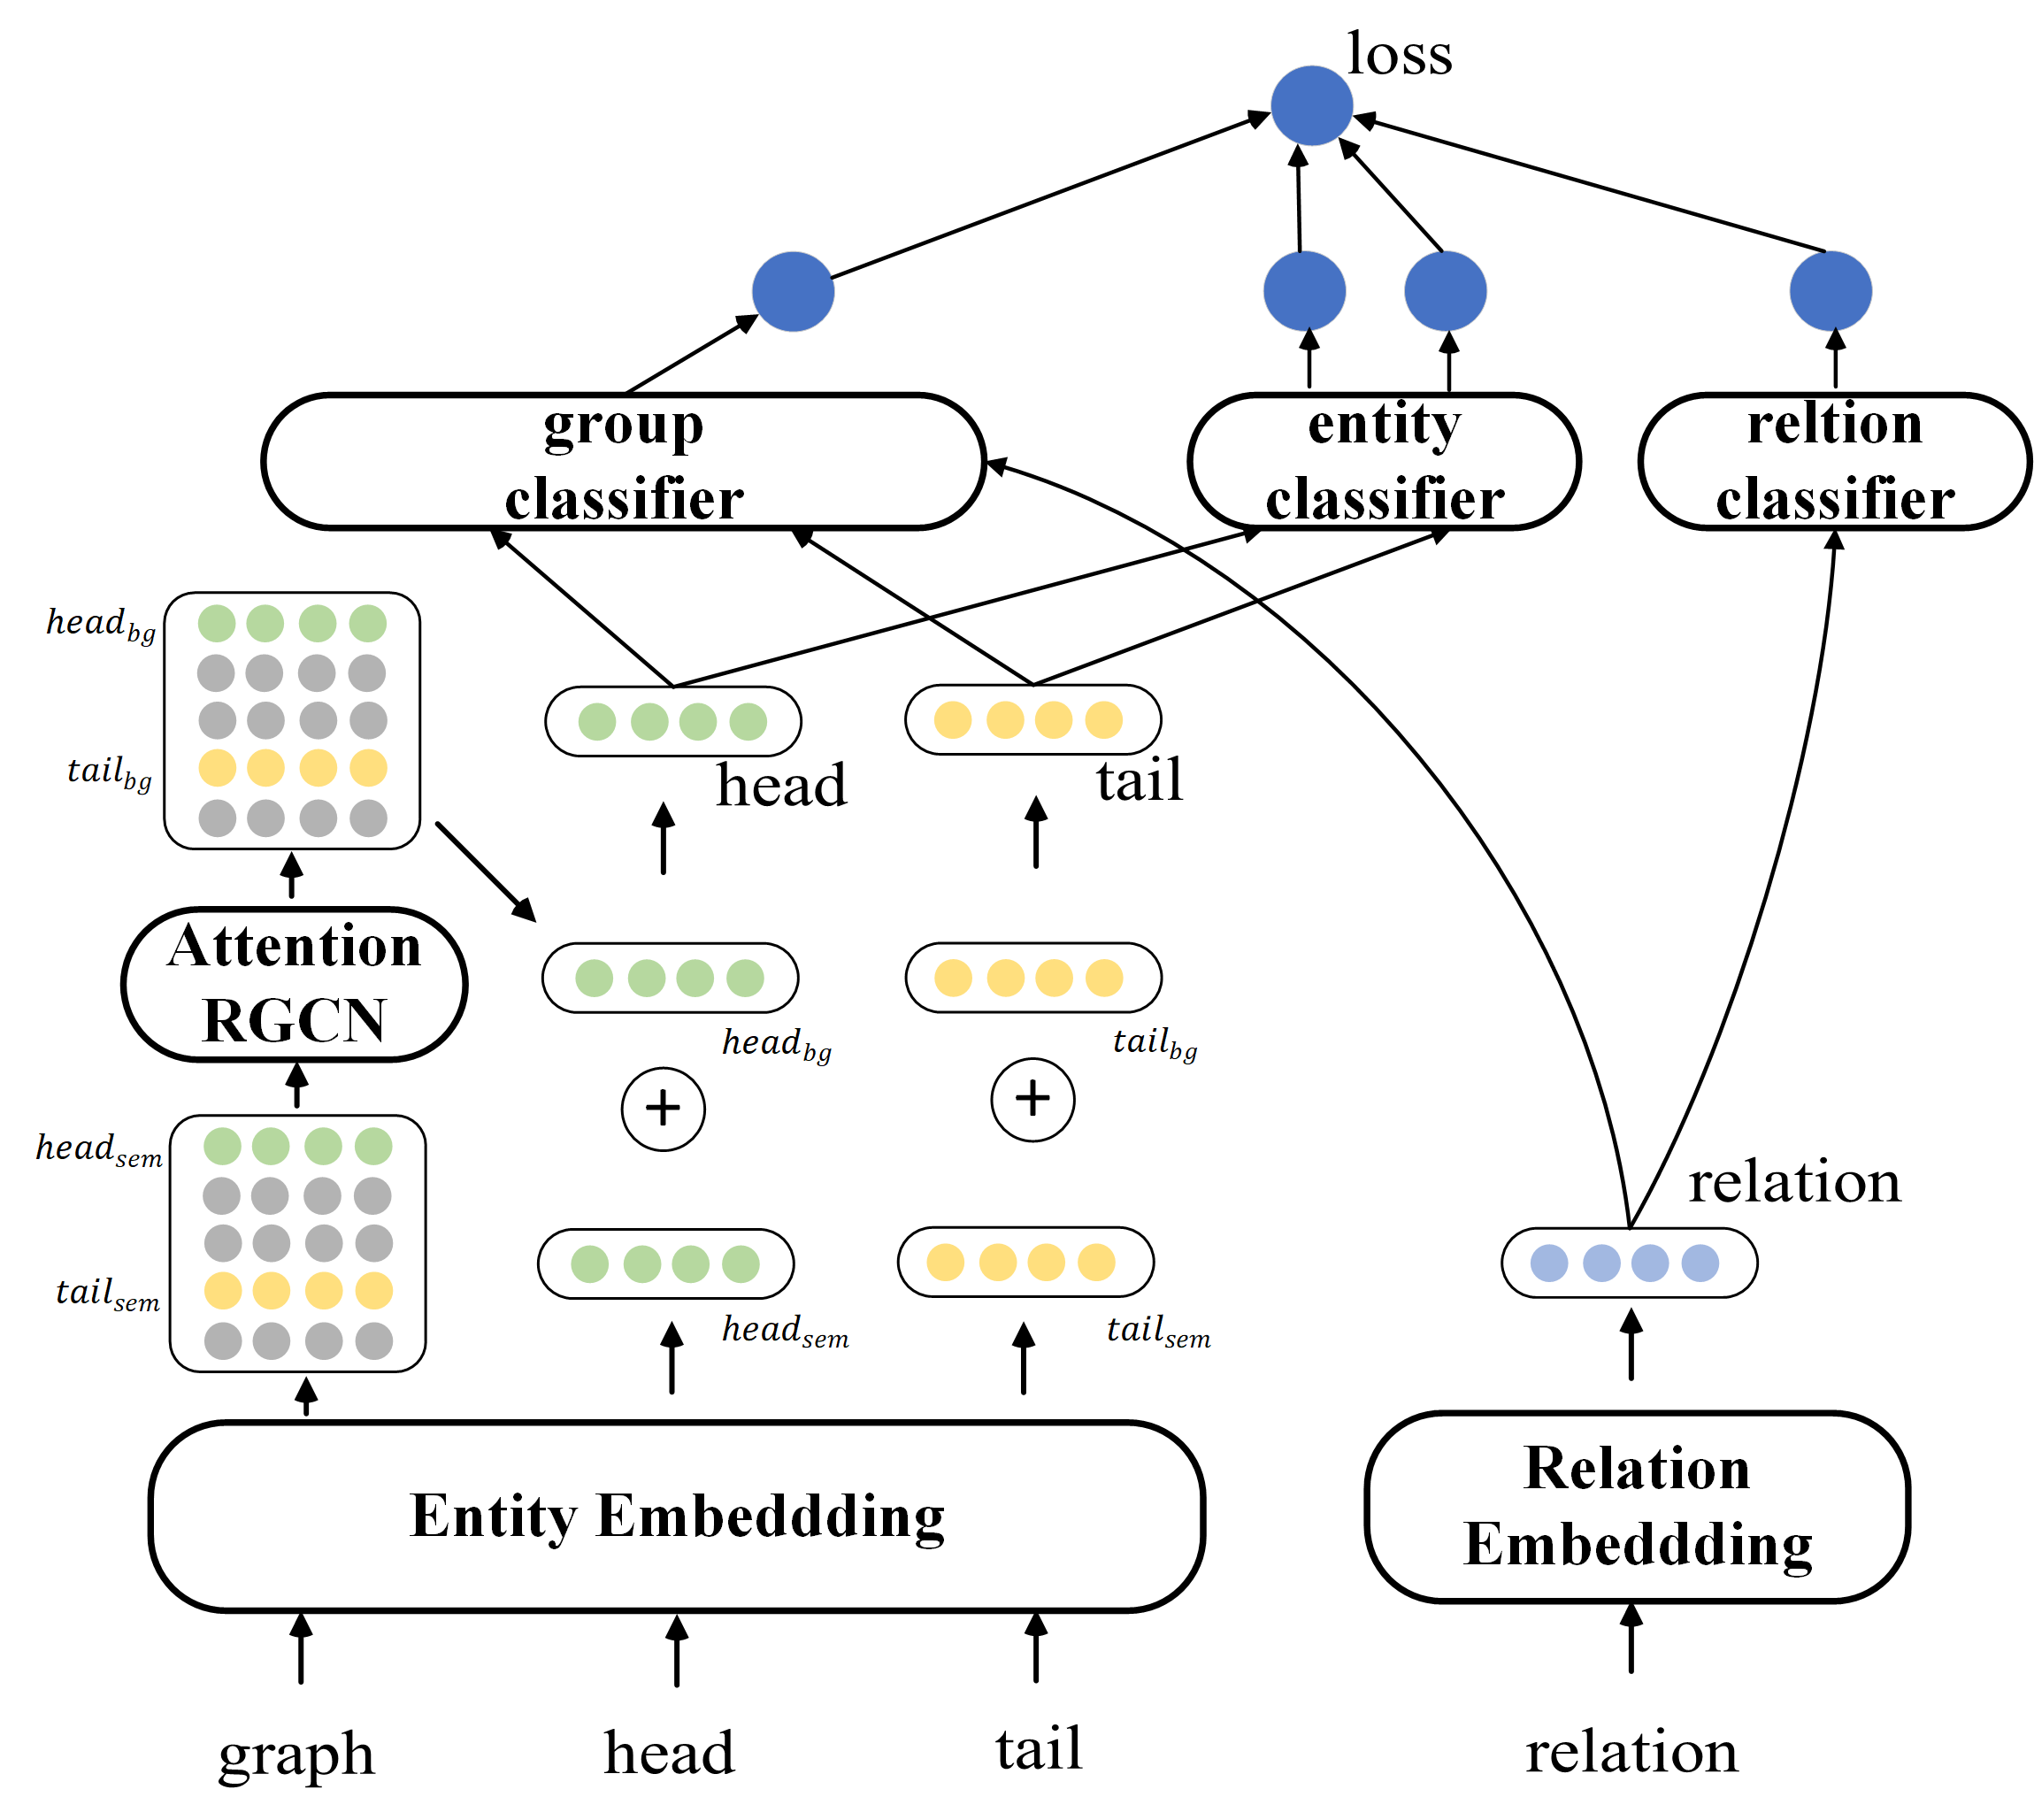
\includegraphics[width=.65\textwidth]{kg-representation.png}
    \caption{组件-事件知识图谱表示学习模型\label{kg-representation}}
\end{figure}

在嵌入层,模型的输入除了三元组$(head, relation, tail)$还有该三元组所在的上下文图$graph$,即$(graph, head,rlation,tail)$。在输入数据前,若三元组为$graph$中存在的,会将$graph$中$head$与$tail$之间的关系$relaion$去掉,防止引入的图结构信息$head_{bg}$与$tail_{bg}$包含了$relation$信息;若三元组中$head$或$tail$不存在于$graph$中,则对应$head_{bg}$或$tail_{bg}$设置为全零。在输入数据后,数据被嵌入层转化为初步向量表示,$graph$被转为了张量矩阵,$head$、$relation$、$tail$则都被转为了单维的向量。初始的嵌入层向量来自于实体、关系的语义信息。具体实现上,使用实体的属性信息对Bert\cite{devlin2018bert}进行预训练,然后每个实体或关系的初始特征向量使用其分词后多个单词的向量均值。

Attention-RGCN层主要在RGCN模型中引入了注意力机制。章节\ref{RGCN}已经对RGCN进行了介绍,在进行特征传播时,实体对其上下文实体都赋予了相同的权重。但在组件-事件知识图谱中,实体对其上下文邻居实体是有不同侧重的,如图\ref{graph-example}中$cpu 100\%$和$memory 100\%$导致了$Backoff$的发生,但$memory 100\%$对$Backoff$的发生更具关键性,它意味着$container1$中没有足够的内存满足$ts-train-service$配置文件里规定的启动需求。因此,本文将注意力机制引入图卷积网络的传播过程,如式\ref{attention-rgcn}所示。
\begin{equation}
    h_{i}^{(l+1)}=\sigma\left(\sum_{r \in \mathcal{R}} \sum_{j \in \mathcal{N}_{i}^{r}} \alpha_{(j, r, i)} \frac{1}{c_{i, r}} W_{r}^{(l)} h_{j}^{(l)}+W_{0}^{(l)} h_{i}^{(l)}\right)
    \label{attention-rgcn}
\end{equation}
本式整体与式\ref{propo-in-directedgraph}一致,各个符号含义此处不进行赘述。其中新引入的$\alpha_{(j, r, i)}$目的在于计算第$i$个结点对其在关系$r$下的邻居结点$j \in \mathcal{N}_{i}^{r}$的注意力权重。其计算公式如下:
\begin{equation}
    v_{(j, r, i)}=\mathbf{W_a}^{T}\left(\mathbf{W_e} h_{j}+\mathbf{W_r} h_{r} + \mathbf{W_e} h_{i}\right)
    \label{group-loss-part1}
\end{equation}
\begin{equation}
    \alpha_{(j, r, i)}=\operatorname{softmax}\left(v_{(j, r, i)}\right)=\frac{\exp \left(v_{(j, r, i)}\right)}{\sum_{j^{\prime} \in \mathcal{N}_{i}^{r}} \exp \left(v_{\left(j^{\prime}, r, i\right)}\right)}
    \label{group-loss-part2}
\end{equation}
式\ref{group-loss-part1}中$h_i,h_j,h_r\in\mathbb{R}^{d}$分别对应索引为$i,j$两实体和关系$r$的嵌入向量,$\mathbf{W_a}\in \mathbb{R}^{d}$,$\mathbf{W_e},\mathbf{W_r} \in \mathbb{R}^{d\times d}$是注意力参数矩阵。最终得到的$ v_{(j, r, i)} \in \mathbb{R}$即为索引为$i$的结点对关系$r$下索引为$j$的结点的注意力权重值。式\ref{group-loss-part2}使用$softmax(.)$函数进一步规范化注意力权重值,其中$\mathcal{N}_{i}^{r}$为索引为$i$的结点在关系$r$下关联的实体索引值集合。经过Attention-RGCN层后可以得到对应索引$i$的实体$head$、对应索引$j$的实体$tail$的上下文图结构嵌入表示$head_{bg}$、$tail_{bg}$,再与通过初步嵌入层的语义向量$head_{sem}$、$tail_{sem}$累加即可,得到同时融入了语义信息和上下文图结构信息的嵌入表示$head_{new}$、$tail_{new}$。

实体分类器用于对实体进行分类,类别标签包括$contanier$、$event$、$service$等共计$c_{n}$个。输入为经过Attention-RGCN得到的融合了语义及上下文图结构信息的嵌入表示$head_{new}$、$tail_{new}$。随后将$head_{new}$、$tail_{new}$输入$d \times h \times c_{n}$的多层感知机和$softmax(.)$层,即可得到实体对各类分类情况。损失函数使用交叉熵,如式\ref{my_entity_loss}所示。其中,$i$、$j$对应着$head$、$tail$两实体的索引号,$h_i$、$h_j$为两实体在网络模型中的输出,$y_i$、$y_j$为两实体的标注向量,$k$表示向量第$k$维度。
\begin{equation}
    \mathcal{L}_{entity}= - \sum_{k=1}^{K} y_{i k} \ln h_{i k} - \sum_{k=1}^{K} y_{j k} \ln h_{j k}
    \label{my_entity_loss}
\end{equation}

关系分类器用于对关系向量分类,类别包括$cause$、$happen$、$hold$等。与实体分类一样,使用多层感知机、$softmax(.)$层分类,然后损失函数使用交叉熵即可,如式\ref{my_relation_loss}所示。其中,$h_r$为关系$relation$对应的网络输出向量,$y_r$为关系的标注向量,$k$表示向量第$k$维度。
\begin{equation}
    \mathcal{L}_{relation}=- \sum_{k=1}^{K} y_{r k} \ln h_{r k}
    \label{my_relation_loss}
\end{equation}

三元组分类器用于判别三元组是否存在,可以使用文献\parencite{trouillon2016complex}中形如式\ref{attention-rgcn-group-score}的评分函数。其中$\operatorname{diag}\left(.\right)$将$h_r\in\mathbb{R}^{d}$中每一个元素当作二维矩阵的对角线元素,从而得到$\mathbb{R}^{d}\times \mathbb{R}^{d}$的二维矩阵。损失函数使用交叉熵,如式\ref{my_group_loss}所示。其中$\mathcal{T}$表示所有的输入$(g, i, r, j)$集合,$l(.)$为激活函数,$y$为三元组是否成立的标签,$g$为三元组$(i, r, j)$所在的上下文图结构。
\begin{equation}
    f(h_{j}, h_{r}, h_{i})=h_{j}^{T} \operatorname{diag}\left(h_{r}\right) h_{i}
    \label{attention-rgcn-group-score}
\end{equation}

\begin{equation}
    \mathcal{L}_{group}= -\frac{1}{|\mathcal{T}|}  \sum_{(g, i, r, j) \in \mathcal{T}} y \log l(f(h_i, h_r, h_j))+(1-y) \log (1-l(f(h_i, h_r, h_j)))
    \label{my_group_loss}
\end{equation}

\subsection{模型训练}\label{representation-paras-learn}
根据上一小节所述,本模型的损失函数为实体分类器、关系分类器、三元组分类器三部分损失函数之和。最终本模型的损失函数如式\ref{represent-loss-all}所示,各个符号含义已在上文进行了描述:

\begin{equation}
    \begin{aligned}
    \mathcal{L}=-\frac{1}{|\mathcal{T}|}&  \sum_{(g, i, r, j) \in \mathcal{T}} y \log l(f(h_i, h_r, h_j))+(1-y) \log (1-l(f(h_i, h_r, h_j)))\\
    &- \sum_{k=1}^{K} y_{i k} \ln h_{i k} - \sum_{k=1}^{K} y_{j k} \ln h_{j k}\\
    &- \sum_{k=1}^{K} y_{r k} \ln h_{r k}\\
    \end{aligned}
    \label{represent-loss-all}
\end{equation}

根据以上损失函数计算的损失值,就可以利用梯度下降算法更新模型参数,直到模型训练完成。模型训练算法如\ref{repre-alg}所示。
\begin{algorithm}[htbp]
	\renewcommand{\algorithmicrequire}{\textbf{输入:}}
	\renewcommand{\algorithmicensure}{\textbf{输出:}}
	\caption{组件-事件知识图谱动态表示学习模型的训练算法}
	\label{repre-alg}
	\begin{algorithmic}[1]
		\REQUIRE 四元组$(graph,head,relation,tail)$集合$D$,学习率$\alpha$,训练代数$epoch$
		\ENSURE 更新后的模型参数$\theta$
		\STATE 随机初始化模型参数$\theta$,$e \gets 0$
		\WHILE {$e<{epoch}$}
            \FORALL{$(graph,head,relation,tail) \in D$}
                \IF {$(head,relation,tail) \in graph$}                        %条件语句
                    \STATE 将$(head,relation,tail)$从$graph$中去除
                \ENDIF
                \STATE ${graph}_{sem}, {head}_{sem}, {tail}_{sem}, {relation}_{sem} \gets \operatorname{Embedding}(graph,head,relation,tail)$
                \STATE ${head}_{bg} \gets 0$, ${tail}_{bg} \gets 0$ 
                \IF {$head,tail \in graph$}          
                    \STATE ${head}_{bg}, {tail}_{bg} \gets \operatorname{Attention-RGCN}({graph}_{sem})$
                \ENDIF
                \STATE ${head}_{new} \gets {head}_{bg} + {head}_{sem}$,${tail}_{new} \gets {tail}_{bg} + {tail}_{sem} $
                \STATE 如式\ref{represent-loss-all}计算损失值$\mathcal{L}_{\theta }\left(graph,head,relation,tail \right)$
                \STATE $\theta \gets \theta - \alpha \nabla \mathcal{L}_{\theta }\left(graph,head,relation,tail \right)$
            \ENDFOR
        \ENDWHILE 
		\STATE \textbf{return} $\theta$
	\end{algorithmic}  
\end{algorithm}
% \begin{algorithm}
%     %\SetAlgoRefName{} % no count number
%     \caption{pISTA}
%     \label{alg:pISTA}
%     Parameters: $\lambda, \gamma$\;
%     Initialization: $x_0$\;
%     \While{not converge}{
%         $x_{k+1}=\Psi^*T_{\lambda\gamma}(\Psi(x_k+\gamma \mathcal{F}^{-1}Q_p(y-Q_p \mathcal{F}x_k)))$\;
%     }
% \end{algorithm}

\subsection{模型预测}
对组件-事件知识图谱进行表示学习后,可以进行抽象事件预测(预测在已发生抽象事件情况下是否会在某组件上发生某种事件)。本质上,就是在给定上下文图结构$g$下,三元组$(i, r, j)$是否成立。

将上下文图结构、头实体、关系和候选尾实体$g$、$(i, r, j)$输入表示学习模型中,会得到该三元组成立的评分,将评分最高的三元组对应的尾实体作为预测抽象事件即可,如式\ref{predict-next-event}所示,其中$events$为候选抽象事件索引集,其它符号含义已在上文进行了描述。

\begin{equation}
    e = \mathop{\arg\max}\limits_{j\in events}( f (h_i, h_r, h_j)) 
    \label{predict-next-event}   
\end{equation}


\section{实验与分析}\label{representation-experiment}
在本节中,对本章提出的组件-事件知识图谱表示学习模型进行了实验与分析。
\subsection{数据集构建}
如实际运维场景一样,本文将模拟收集的数据划分成了历史数据和实时数据。具体上,模拟收集的所有数据会首先按照故障类型分组。然后,每种故障类型下的时间段集合会被划分成历史故障数据和实时故障数据,如表\ref{anomal-split}所示。

\begin{table}[htbp]
    \caption{模拟数据划分}
    \centering
    \label{anomal-split}
    \begin{tabular}{cccc}
    \toprule[1.5pt]
                分布式应用 & \begin{tabular}[c]{@{}c@{}}模拟故障\\ 时间段总数\end{tabular} & \begin{tabular}[c]{@{}c@{}}历史故障\\ 时间段数\end{tabular} & \begin{tabular}[c]{@{}c@{}}实时故障\\ 时间段数\end{tabular} \\ \midrule[1.5pt]
    train-ticket & 471                                                  & 325                                                 & 146                                                 \\
    sock-shop    & 539                                                  & 371                                                 & 168                                                 \\ \bottomrule[1.5pt]
    \end{tabular}
\end{table}

根据章节\ref{event-cause-classidier-experiment}事件因果关系判别实验结果,本处选用SVM模型从每类故障对应的历史故障数据中挖掘事件因果对,再按照章节\ref{graph-generate}所示步骤沉淀生成每类故障的组件-事件知识图谱。由模型初步生成的知识图谱虽然满足了实际使用需求,但不能保证没有任何瑕疵。因此,后续运维专家参与了知识图谱调优,保证了知识图谱绝对无瑕。在调优过程中,因为本文方法初步生成的知识图谱含有实体、关系量级低,所以知识图谱调优过程消耗人工较少。

表\ref{kg-abstract-event-num}统计了两个分布式应用每类故障类型所对应组件-事件知识图谱的抽象事件实体数目及抽象事件因果关系对数。在每张组件-事件知识图谱中,由于每个抽象事件实体都对应着一个组件实体,所以组件到抽象事件的发生关系数量与抽象事件节点数相等;由于组件层实体数量和关系数量只与分布式应用有关,所以每个组件-事件知识图谱的组件层关系数是恒定的。train-ticket组件层关系数为1469,sock-shop组件层关系数为1043。

\begin{table}[htbp]
    \centering
    \caption{知识库三元组数目及划分}
    \label{triple-split}
    \begin{tabular}{cccccccc}
    \toprule[1.5pt]
    分布式应用        & \begin{tabular}[c]{@{}c@{}}组件层\\ 三元组数\end{tabular} & \begin{tabular}[c]{@{}c@{}}组件-事件间\\ 三元组数\end{tabular} & \begin{tabular}[c]{@{}c@{}}事件层\\ 三元组数\end{tabular} & \begin{tabular}[c]{@{}c@{}}总\\ 三元组数\end{tabular} & 训练集  & 验证集 & 测试集 \\ \midrule[1.5pt]
    train-ticket & 1469                                               & 339                                                   & 1182                                               & 2990                                             & 1794 & 598 & 598 \\
    sock-shop    & 1043                                               & 563                                                   & 3089                                               & 4695                                             & 2817 & 939 & 939 \\ \bottomrule[1.5pt]
    \end{tabular}
\end{table} 

在知识图谱中,一个关系对应着一个三元组,所以直接将各个组件-事件知识图谱中的每个关系对应的三元组视作正样本,即将其标注为“成立”。其中组件层的关系不会被重复使用,防止数据不均衡。表\ref{triple-split}为本块实验使用的正样本三元组数量,和按照6:2:2划分数据集的结果。另外,对于每一个正样本三元组,可以将其首实体或尾实体随机替换为不匹配的实体,构成负样本三元组,即“不成立”的三元组。

\begin{table}[htbp]
    \caption{各类故障对应知识图谱信息}
    \centering
    \label{kg-abstract-event-num}
    \begin{tabular}{cccc}
    \toprule[1.5pt]
    分布式应用          & 故障代号                                    & 抽象事件节点数目 & 抽象事件因果关系数目 \\ \midrule[1.5pt]
                 & f1                                      & 41       & 285        \\
                 & f2                                      & 39       & 297        \\
                 & f3                                      & 6        & 8          \\
                 & f5                                      & 62       & 81         \\
    train-ticket & f6                                      & 34       & 233        \\
                 & f10                                     & 15       & 51         \\
                 & f13                                     & 15       & 15         \\
                 & f16                                     & 35       & 59         \\
                 & f17                                     & 38       & 65         \\
                 & f18                                     & 54       & 88         \\ \midrule[1pt]
                 & db\_goods\_disappeared                  & 20       & 86         \\
                 & db\_cart\_disappeared                   & 70       & 638        \\
                 & user\_unable\_log\_in                   & 52       & 180        \\
                 & db\_order\_disappeared                  & 20       & 114        \\
                 & order\_cart\_500                        & 9        & 8          \\
                 & order\_count\_500                       & 55       & 536        \\
                 & order\_payment\_500                     & 13       & 30         \\
                 & user\_register\_500                     & 7        & 6          \\
    sock-shop    & cart\_disappeared                       & 4        & 5          \\
                 & catalogue\_goods\_disappeared           & 6        & 7          \\
                 & add\_cart\_delay                        & 30       & 57         \\
                 & user\_register\_and\_log\_in\_delay     & 17       & 43         \\
                 & check\_order\_delay                     & 102      & 598        \\
                 & net\_loss\_check\_order                 & 92       & 614        \\
                 & net\_loss\_add\_cart                    & 34       & 79         \\
                 & net\_loss\_user\_register\_and\_log\_in & 17       & 55         \\
                 & net\_loss\_goods\_appear\_delay         & 15       & 33         \\ \bottomrule[1.5pt]
    \end{tabular}
\end{table}

% 随后的实验中,数据的输入形式为三元组$(head,relation,tail)$及其所在上下文图结构$graph$。

\subsection{评测指标}
在知识图谱表示学习模型评测方式中有两个被广泛使用的任务。

\textbf{任务1}:链接预测,即预测受损三元组中缺少的头或尾实体。文献\parencite{bordes2011learning,bordes2013translatingE}定义链接预测为给定$(head,relation)$或$(relation,tail)$预测对应丢失的$tail$或$head$。在具体进行链接预测任务时,实验会排序候选实体集合,而不是直接只输出一个最佳匹配实体。

具体上,依据文献\parencite{bordes2013translatingE}的做法,对于每一个测试三元组$(head,relation,tail)$,实验会使用实体集合中任意不匹配$(relation,tail)$(或$(head,relation)$)的实体来替换$head$(或$tail$)生成受损三元组,然后根据模型输出的三元组成立概率分数降序排列这些三元组。在获得所有三元组排名后,实验使用了两个衡量指标:正确实体的平均排名(即MR,mean rank);正确实体在前N名的占比(即Hits at n,Hits@n)。MR越小,Hits@N越大,都意味着表示模型效果越好。另外,文献\parencite{bordes2013translatingE}发现生成的受损三元组可能是正确三元组,所以需要将该三元组筛选过滤掉。而本文中,由于知识图谱已被调优过,每个正确三元组都在对应$graph$中完备地存在着,当实体与$(relation,tail)$(或$(head,relation)$)不匹配时(不存在于组件-事件知识图谱中)意味着其生成的受损三元组一定是错误的,所以本块实验不需进行过滤操作。
% 最终,train-ticket中每个正确三元组会生成1404个受损三元组,sock-shop中每个正确三元组会生成1238个受损三元组。

\textbf{任务2}:三元组分类,即判断给定的三元组是否是知识图谱中真实存在的。在三元组分类任务中,给定知识图谱$graph$和三元组$(head,relation,tail)$,需要判断它是否是正确的。该任务已经在已有的工作\cite{bordes2013translatingE,wang2014knowledge,lin2015learning}中展开过,也被广泛的应用在很多自然语言处理场景,比如问答。

链接预测时,输入候选实体和上下文信息,输出三元组成立的概率,成立概率值越大排名越高,再计算对应的MR和Hits@N即可。三元组分类时,输入待测三元组及其上下文,输出该三元组是否成立,再计算精确率(precision)、召回率(recall)和F1值即可。


% 我们首先对标准链路预测任务中的不同嵌入模型进行了比较研究,即预测不可见三胞胎的正确性。如(Bordes et al.,2013b)中所述,我们将链接预测作为实体排序任务。对于测试数据中的每个三元组,我们依次将每个实体作为要预测的目标实体。计算字典中正确实体和所有损坏实体的分数,并按降序排列。我们考虑平均倒数秩(MRR)(一个回答实体的倒数秩在所有测试三元组上的平均值),命中@10(前10名精度)和平均精度(MAP)(如(Chang等人,2014年)中所用)作为评估指标(from EMBEDDING ENTITIES AND RELATIONS FOR LEARN-
% ING AND INFERENCE IN KNOWLEDGE BASES
% )
\subsection{实验方法}
本块实验选取了多个对比方法以验证本文模型的优越性。实验记录了选取的每个方法在上小节两个评测任务上的表现指标。所选取的各个方法如下所示:
\begin{itemize}[itemsep=0 pt,topsep = 0 pt,parsep =0pt,partopsep=0pt]
    \item [(1)] 
    \textbf{TransE}\cite{bordes2013translatingE}:TransE将每个三元组(head,relation,tail)中的relation视作从head到tail的翻译过程。
    \item [(2)]
    \textbf{TransH}\cite{wang2014knowledge}:TransH将头尾实体都投影到关系所在的张量空间中,可以解决复杂的一对多、多对多关系。
    \item [(3)]
    \textbf{TransR}\cite{lin2015learning}:TransR将关系也嵌入为矩阵,可以区分具有不同语义的关系。
    \item [(4)]
    \textbf{GAKE}\cite{feng2016gake}:GAKE引入邻居上下文、边上下文、路径上下文信息,可以捕获图结构的语义。
    \item [(5)]
    \textbf{TCE}\cite{shi2017knowledge}:TCE引入了两种结构信息,一种是实体的相邻实体,另一种是一对实体之间的关系路径。
    \item [(6)]
    \textbf{DKGE}:本文在章节\ref{chapter-3}所提出的组件-事件知识图谱表示学习模型。
    \item [(7)]
    \textbf{DKGE-1}:相比本文表示学习方法,去除了Attention-RGCN层的注意力机制。
    \item [(8)]
    \textbf{DKGE-2}:相比本文表示学习方法,去除实体分类模块的损失。
    \item [(9)]
    \textbf{DKGE-3}:相比本文表示学习方法,去除关系分类模块的损失。
  \end{itemize}

其中,TransE、TransH和TransR将每个三元组视作一条独立的知识,用于对比验证引入上下文结构信息对表示学习的提升;GAKE、TCE引入上下文结构信息获取静态表示向量,用于对比验证动态表示学习的有效性;DKGE-1使用无attention机制的RGCN,用于对比验证本文在RGCN中引入注意力机制的提升;DKGE-2去除实体分类模块,用于对比验证引入实体类别信息对模型的提升;DKGE-3去除关系分类模块,用于对比验证关系类别信息对模型的提升。

\subsection{实验结果与分析}
% \begin{table}[htbp]
%     \centering
%     \caption{链接预测结果}
%     \label{link-predict-result}
%     \begin{tabular}{ccccc}
%     \hline
%     方法     & MRR         &             & HIT@10        & H10 raw       \\ \hline
%     TransE & 125         & 243         & 47.1          & 34.9          \\
%     TransH & 84          & 211         & 58.5          & 42.5          \\
%     TransR & 77          & 198         & 68.7          & 48.2          \\
%     GAKE   & 119         & 228         & 64.8          & 44.5          \\
%     TCE    & 25          & 110         & 83.1          & 55.3          \\
%     本文方法   & \textbf{17} & \textbf{86} & \textbf{85.4} & \textbf{59.4} \\
%     本文方法-1 & 24          & 124         & 82.6          & 52.1          \\ \hline
%     \end{tabular}
% \end{table}
% \begin{table}[htbp]
%     \caption{链接预测结果}
%     \centering
%     \label{link-predict-result}
%     \begin{tabular}{ccc}
%     \hline
%     方法     & MR                          & Hits@3                         \\ \hline
%     TransE & 121                          & 48.3                           \\
%     TransH & 83                           & 57.3                           \\
%     TransR & 71                           & 66.2                           \\
%     GAKE   & 76                           & 62.8                           \\
%     TCE    & 32                           & 81.9                           \\
%     本文方法   & \textbf{17} & \textbf{85.4} \\
%     本文方法-1 & 24                           & 82.6                           \\ \hline
%     \end{tabular}
% \end{table}


在链接预测任务上,表\ref{link-predict-result}列出了各个方法的链路预测结果。DKGE在MR和Hit@5指标上都得到了比其他方法更好的实验结果。在三元组分类任务上,表\ref{triple-class-result}列出来各个方法的精确率(precision)、召回率(recall)和F1值。DKGE相较基线方法获得了5\%以上的F1值提升。实验结果证明了本文利用注意力机制的RGCN获取图结构上下文信息,再结合语义信息的动态表示学习方法,可以更好地嵌入表示组件-事件知识图谱。
\begin{table}[htbp]
    \caption{链接预测结果}
    \centering
    \label{link-predict-result}
    \begin{tabular}{ccccc}
    \toprule[1.5pt]
           & \multicolumn{2}{c}{train-ticket} & \multicolumn{2}{c}{sock-shop} \\
    方法     & MR            & Hits@5           & MR           & Hits@5         \\ \midrule[1.5pt]
    TransE & 59            & 48.3             & 63           & 42.7           \\
    TransH & 42            & 57.3             & 56           & 45.2           \\
    TransR & 37            & 66.2             & 43           & 59.8           \\
    GAKE   & 33            & 62.8             & 39           & 53.2           \\
    TCE    & 23            & 81.9             & 31           & 78.1           \\
    DKGE   & \textbf{9}    & \textbf{85.4}    & \textbf{13}  & \textbf{82.9}  \\
    DKGE-1 & 26            & 79.5             & 34           & 67.6         \\ 
    DKGE-2 & 19           & 82.2             & 30           & 78.4           \\ 
    DKGE-3 & 16            & 83.6            & 24           & 81.2          \\ 
    \bottomrule[1.5pt]
    \end{tabular}
\end{table}

\begin{table}[htbp]
    \caption{三元组分类结果}
    \centering
    \label{triple-class-result}
    \begin{tabular}{ccccccc}
    \toprule[1.5pt]
               &                & train-ticket   &                &                & sock-shop      &                \\
    方法         & precision      & recall         & F1             & precision      & recall         & F1             \\ \midrule[1.5pt]
    TransE     & 0.650          & 0.692          & 0.670          & 0.653          & 0.626          & 0.639          \\
    TransH     & 0.703          & 0.730          & 0.716          & 0.707          & 0.675          & 0.691          \\
    TransR     & 0.743          & 0.716          & 0.730          & 0.680          & 0.701          & 0.690          \\
    GAKE       & 0.781          & 0.749          & 0.765          & 0.722          & 0.742          & 0.732          \\
    TCE        & 0.804          & 0.783          & 0.793          & 0.736          & 0.769          & 0.752          \\
    DKGE   & \textbf{0.864} & \textbf{0.837} & \textbf{0.850} & \textbf{0.836} & \textbf{0.814} & \textbf{0.825} \\
    DKGE-1 & 0.763          & 0.816          & 0.788          & 0.776          & 0.746          & 0.761          \\
    DKGE-2 & 0.826          & 0.801          & 0.813          & 0.783          & 0.808          & 0.795          \\
    DKGE-3  & 0.845          & 0.822          & 0.834          & 0.788          & 0.810           & 0.799          \\ \bottomrule[1.5pt]
    \end{tabular}
\end{table}

对比DKGE-1、DKGE-2、DKGE-3,可发现图神经网络的注意力机制对模型的提升效果最大,其可以强化重要信息的传播、挖掘重要的图结构信息;实体、关系类别信息的引入也可以改善知识表示学习效果,其中实体类别信息比关系类别信息重要性更高。

另外,DKGE在三元组分类任务上取得的精确率要比链接预测上Hits@5要高,原因在于三元组分类任务中每个“成立”的三元组都只生成$\omega$个“不成立”的受损三元组(本实验中$\omega$取100);而链接预测任务中,每个正确三元组与平均约1000个受损三元组进行比较排序。

本块实验中,本文模型达到最佳效果时使用的超参为:嵌入层维度为100;Attention-RGCN为4层、输入窗口大小为128节点,中间隐状态维度为50、输出隐状态维度为100;实体分类器结构为$100*32*7$,7为实体种类数;关系分类器结构为$100*32*8$,8为关系种类数。
\section{本章小结}
本章主要介绍了组件-事件知识图谱的表示学习模型,通过将实体表示分为结构特征和语义特征,其中拓扑结构特征通过Attention-RGCN获取,语义特征使用实体分词对应词向量均值表示,从而实现了实体在不同拓扑上下文的动态表示。同时也介绍了优化目标和预测事件的公式。实验结果验证了本章表示学习模型的有效性。

% 1、基于 h r t 三元组
% 相关工作:基于path的那种
% 本文:将上下文考虑进去,上下文要么 (hrt)集合  要么图(ve)
% loss:分类,三元组判别对不对
% 评判标准:链路预测、实体分类

% 2、基于 网络表示学习 的那种
% 相关工作:基于rgcn的那种
% 本文:将上下文考虑进去,上下文要么 (hrt)集合  要么图(ve)
% loss:分类,三元组判别对不对
% 评判标准:关系预测、结点分类




\chapter{基于知识图谱的故障预测}
本章节主要介绍基于知识图谱的故障预测模型。在云计算场景中,分布式集群会随时间产生大量的事件序列。本文提出的故障预测模型可以利用已发生的事件序列,并结合知识图谱,预测是否会有故障产生以及具体产生何种故障,有助于运维人员提前检测、调整系统,防止故障真正发生而带来损失。具体实现上,该模型通过双向记忆网络获取实时事件序列编码表示,再使用上一章的表示学习模型获取知识图谱嵌入表示,最后将两者通过注意力权重计算相似度值,相似度值最高的知识图谱对应的故障信息即为所预测的故障。本模型在进行故障预测时取得了最高的准确率,且具有更高的细粒度与更好的可解释性。
\section{场景分析}
目前已经存在着较多相关的工作,但主要集中在研究数据的时序性。文献\parencite{pitakrat2018hora,zhang2018prefix,baldoni2015line}使用了统计学习和机器学习方法,如隐半马尔可夫模型(HSMM)、支持向量机(SVM)。然而,HSMM和SVM都建立于所有输入都是平稳且相互独立的假设之上,这种假设在云计算场景中是不成立的,因为云计算场景中不同组件产生的事件信息之间会存在一定的关联,比如先后时间顺序。为了处理时间序列数据进行故障预测,文献\parencite{xu2016health,cheng2018machine,du2017deeplog,das2018desh,islam2017predicting}使用深度学习方法如卷积神经网络(RNN)和长短期记忆神经网络(LSTM)进行预测。但RNN存在着难以克服的缺点,它会遗忘掉较远距离的数据信息。LSTM则克服了这个缺点,可以通过记忆门依然保留长距离数据的信息。文献\parencite{cheng2018machine,du2017deeplog,das2018desh}等工作已经使用LSTM在故障预测任务上比HSMM、SVM和RNN取得了更高的准确率。上述的方法都使用CPU使用率、内存使用率、未映射页缓存、平均磁盘I/O时间和磁盘使用率作为输入,把系统任务是否会失败作为输出。随后,文献\parencite{gao2020task}在LSTM的基础上使用了多层的Bi-LSTM、引入了任务优先级、提交时间、提交次数等更多的特征,还根据不同数据对故障的重要性赋予其不同的权重。

在本文场景中进行故障预测时,还需要考虑以下场景特性:

1)数据形式为事件序列。本文所有的数据,除了包括上文提到的CPU使用率、内存使用率、未映射页缓存、平均磁盘I/O时间和磁盘使用率,另外还有新引入的微服务启动、重启、程序运行日志等数据,都已经被转为统一规范化的事件数据,所以要处理的数据为事件序列。

2)需要引入知识图谱增强可解释性。本文在进行故障预测时,已经存在了前文所构建的组件-事件知识图谱,所以需要引入知识图谱进行故障预测,这样会使预测结果更具可解释性,还能具体到会预测出现何种故障,而之前的工作只能预测有无故障。
\begin{figure}[htbp]
    \centering
    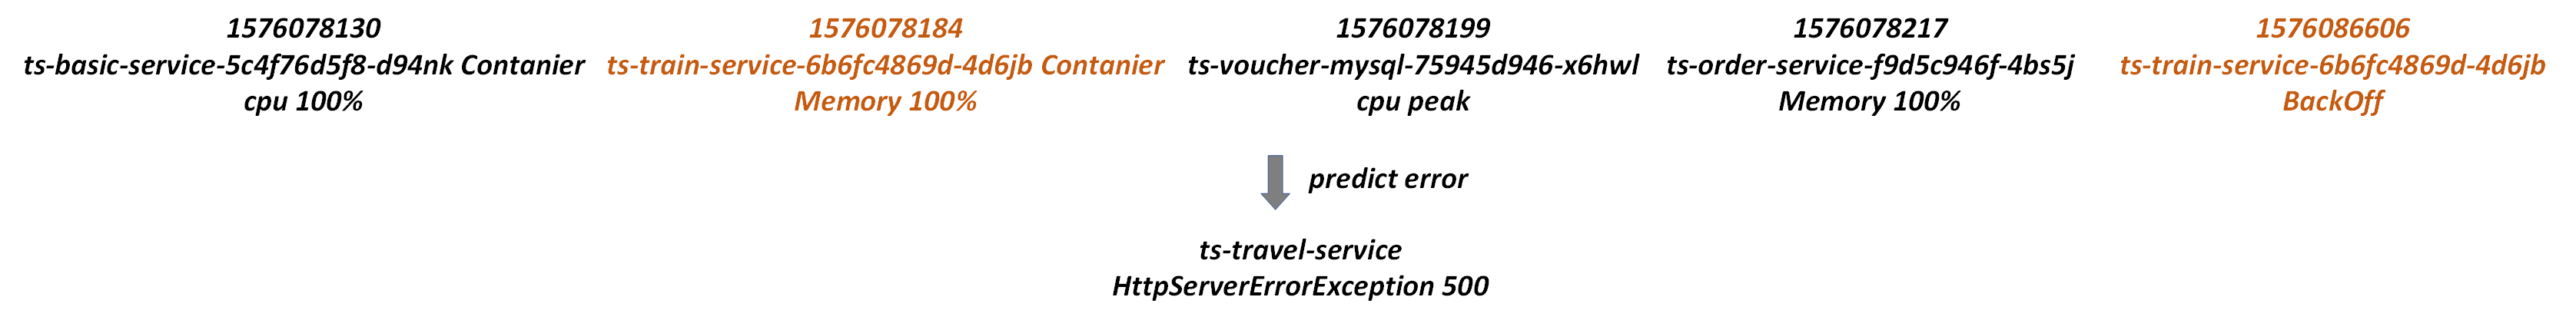
\includegraphics[width=1.0\textwidth]{predict-case.png}
    \caption{事件序列故障预测\label{predict-case}}
\end{figure}

3)事件权重分配需要考虑事件所在的上下文,不能仅根据数据对故障的重要性赋予权重。如图\ref{predict-case}所示是一个实时事件序列案例。在进行故障预测时,并不是每个异常事件都是同等重要的。$ts-train-service-6b6fc4869d-4d6jb$上的$Contanier Memory 100\%$和$ts-train-service-6b6fc4869d-4d6jb$上的$BackOff$事件应当比其他事件的重要性更高,因为这两个事件的发生意味着$ts-train-service$所在的$Container$已经内存不足,使得$ts-train-service$微服务无法正常启动,后续导致$ts-travel-service$发生$  HttpServerErrorException 500$的可能性极高。而其它的事件如$ts-order-service-f9d5c946f-4bs5j$上的$Memory 100\%$虽然对图\ref{order-service-error}的“订票服务不可用”故障较为重要,但是并没有发生后续的关键事件类型$ts-order-service backoff$,所以其重要性较低。

基于以上的分析,本文在编码事件序列时,依然选择基于LSTM的模型,但不同于之前根据每个事件元素对故障重要程度赋予权重\cite{gao2020task},本文选择使用组件-事件知识图谱的嵌入向量来对各个时间单元的数据计算注意力权重,即由组件-事件知识图谱选取其所关注的信息。

\section{基于记忆网络的故障预测算法}\label{memory-net-section}
本小节主要介绍了文献\parencite{gao2020task}在进行故障预测时所使用的记忆神经网络。
\subsection{模型结构}
\begin{figure}[htbp]
    \centering
    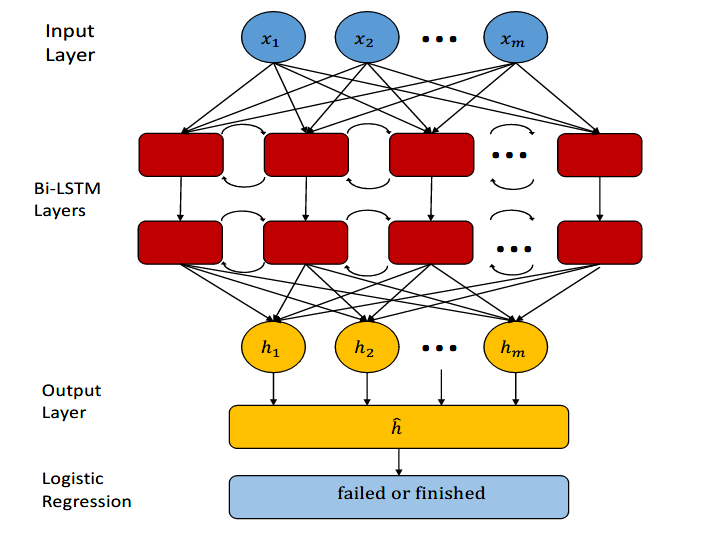
\includegraphics[width=.7\textwidth]{bilstm-model.png}
    \caption{双向记忆网络\label{bilstm-model}}
\end{figure}
图\ref{bilstm-model}所示为双向记忆神经网络,可见其包含输入层、两层Bi-LSTM、输出层和逻辑回归层。

输入层主要是数据的嵌入层。文献\parencite{gao2020task}拼接了同一时间点的CPU使用率、内存使用率、未映射页缓存、平均磁盘I/O时间、磁盘使用率、任务优先级、提交时间和提交次数共计8个特征。这样之后每个时间点都是一个8维的嵌入向量。
\begin{figure}[htbp]
    \centering
    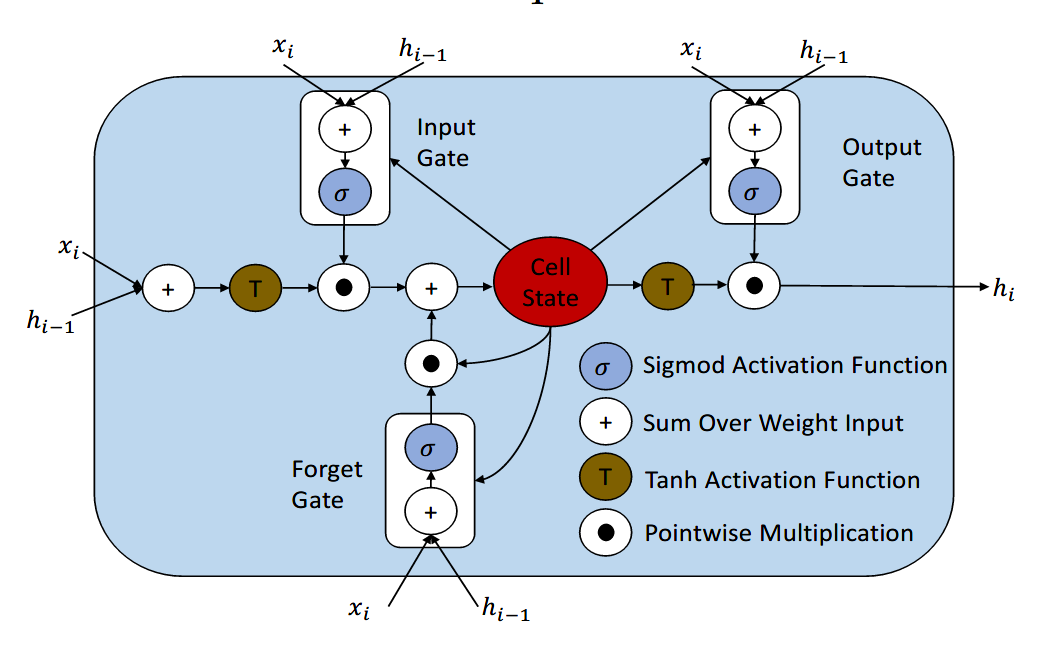
\includegraphics[width=.7\textwidth]{lstm-cell.png}
    \caption{记忆网络单元\label{lstm-cell}}
\end{figure}

Bi-LSTM层完成了对时序数据的特征编码。该层会将输入的时序数据分别进行前向编码和后向编码,再将得到的前向隐状态和后向隐状态拼接得到最终的隐状态。经过上述步骤后,每个时间点的隐状态都会得到正向反向的上下文信息。图\ref{lstm-cell}展示了LSTM神经元内部的结构,可见其主要利用了非线性函数选择数据保存还是舍弃。具体实现上,每个神经元内部共有三个门控制其状态,包括输入门、遗忘门和输出门。输入门决定了应该更新哪个神经元状态,遗忘门决定了应该忽视掉什么信息,输出门决定输出隐状态的哪部分信息。该过程可以用公式\ref{lstm-cell-equation}表示:
\begin{equation}
    \begin{array}{l}
    g_{i}=\varphi\left(w_{g x} x_{i}+w_{g h} h_{i - 1}+b_{g}\right) \\
    n_{i}=\sigma\left(w_{n x} x_{i}+w_{n h} h_{i- 1}+b_{n}\right) \\
    f_{i}=\sigma\left(w_{f x} x_{i}+w_{f h} h_{i- 1}+b_{f}\right) \\
    o_{i}=\sigma\left(w_{o x} x_{i}+w_{o h} h_{i- 1}+b_{o}\right) \\
    s_{i}=g_{i} \odot n_{i}+s_{i -1} \odot f_{i} \\
    h_{i}=\varphi\left(s_{i}\right) \odot o_{i}
    \end{array}
    \label{lstm-cell-equation}
\end{equation}
其中$w_{gx}, w_{nx}, w_{fx} $和$w_{ox} $是记忆单元输入$x_{i}$的权重系数。$w_{gh}, w_{nh}, w_{fh} $和$w_{oh} $是记忆单元上一步输出$h_{i}-1$的权重系数。$b_{g}, b_{n}, b_{f},$ 和 $b_{o}$分别为输入信息$g_{i}$、输入门$n_{i}$、遗忘门$f_{i}$和输出门$o_{i}$对应的偏置系数。而$s_{i}$和$s_{i-1}$则分别为时间$i$和$i-1$的神经元状态。另外,$\odot$代表点乘,$\sigma$代表sigmoid激活函数,$\varphi$代表tanh激活函数。

输出层目的在于将输入序列中每个记忆单元隐状态整合起来。具体方式是将输入$X=\left\{x_{1}, x_{2} \ldots x_{m}\right\}$传入Bi-LSTM得到的表示序列$\left\{h_{1}, h_{2} \ldots h_{m}\right\}$进行式\ref{mean-pool}中所示的平均池化操作,得到序列表示向量$\widehat{h}$。
\begin{equation}
    \widehat{h}=\frac{1}{m} \sum_{i=1}^{m} h_{i}
    \label{mean-pool}
\end{equation}

逻辑回归层是预测当前数据序列将来是否会有故障的二分类器。具体实现上,该层将输出层得到的向量表示$\widehat{h}$输入$\operatorname{logstic}(.)$函数,计算会出现故障的概率。当概率大于阈值时,则预测会出现故障;反之,则预测不会出现故障。

\subsection{模型训练}
基于记忆网络的故障预测模型的最终训练目标为正确分类每种数据序列。对应的损失函数为式\ref{memroy-net-loss}中所示。
\begin{equation}
    \mathcal{L}=-\sum_{i=1}^{n}\left[Y_{i} \log \left(f\left(X_{i} \right)\right)+\left(1-Y_{i}\right) \log \left(1-f\left(X_{i} \right)\right)\right]
    \label{memroy-net-loss}
\end{equation}
其中$X_{i}$表示第$i$条输入序列,$Y_{i}$为$X_{i}$对应的标签,即下一个时间点是否会有故障发生(1代表有故障发生,0代表不会有故障发生)。$f\left(.\right)$表示上文的网络模型。
\section{基于记忆网路和知识图谱的故障预测模型}
本小节主要介绍基于双向记忆网络和组件-事件知识图谱的故障预测模型。在上节已经介绍了编码时序数据的双向记忆网络,本节会进一步引入组件-事件知识图谱辅助故障预测,旨在提高故障预测的细粒度(预测到会出现何种故障)和预测结果可解释性。

\subsection{模型结构}
\begin{figure}[htbp]
    \centering
    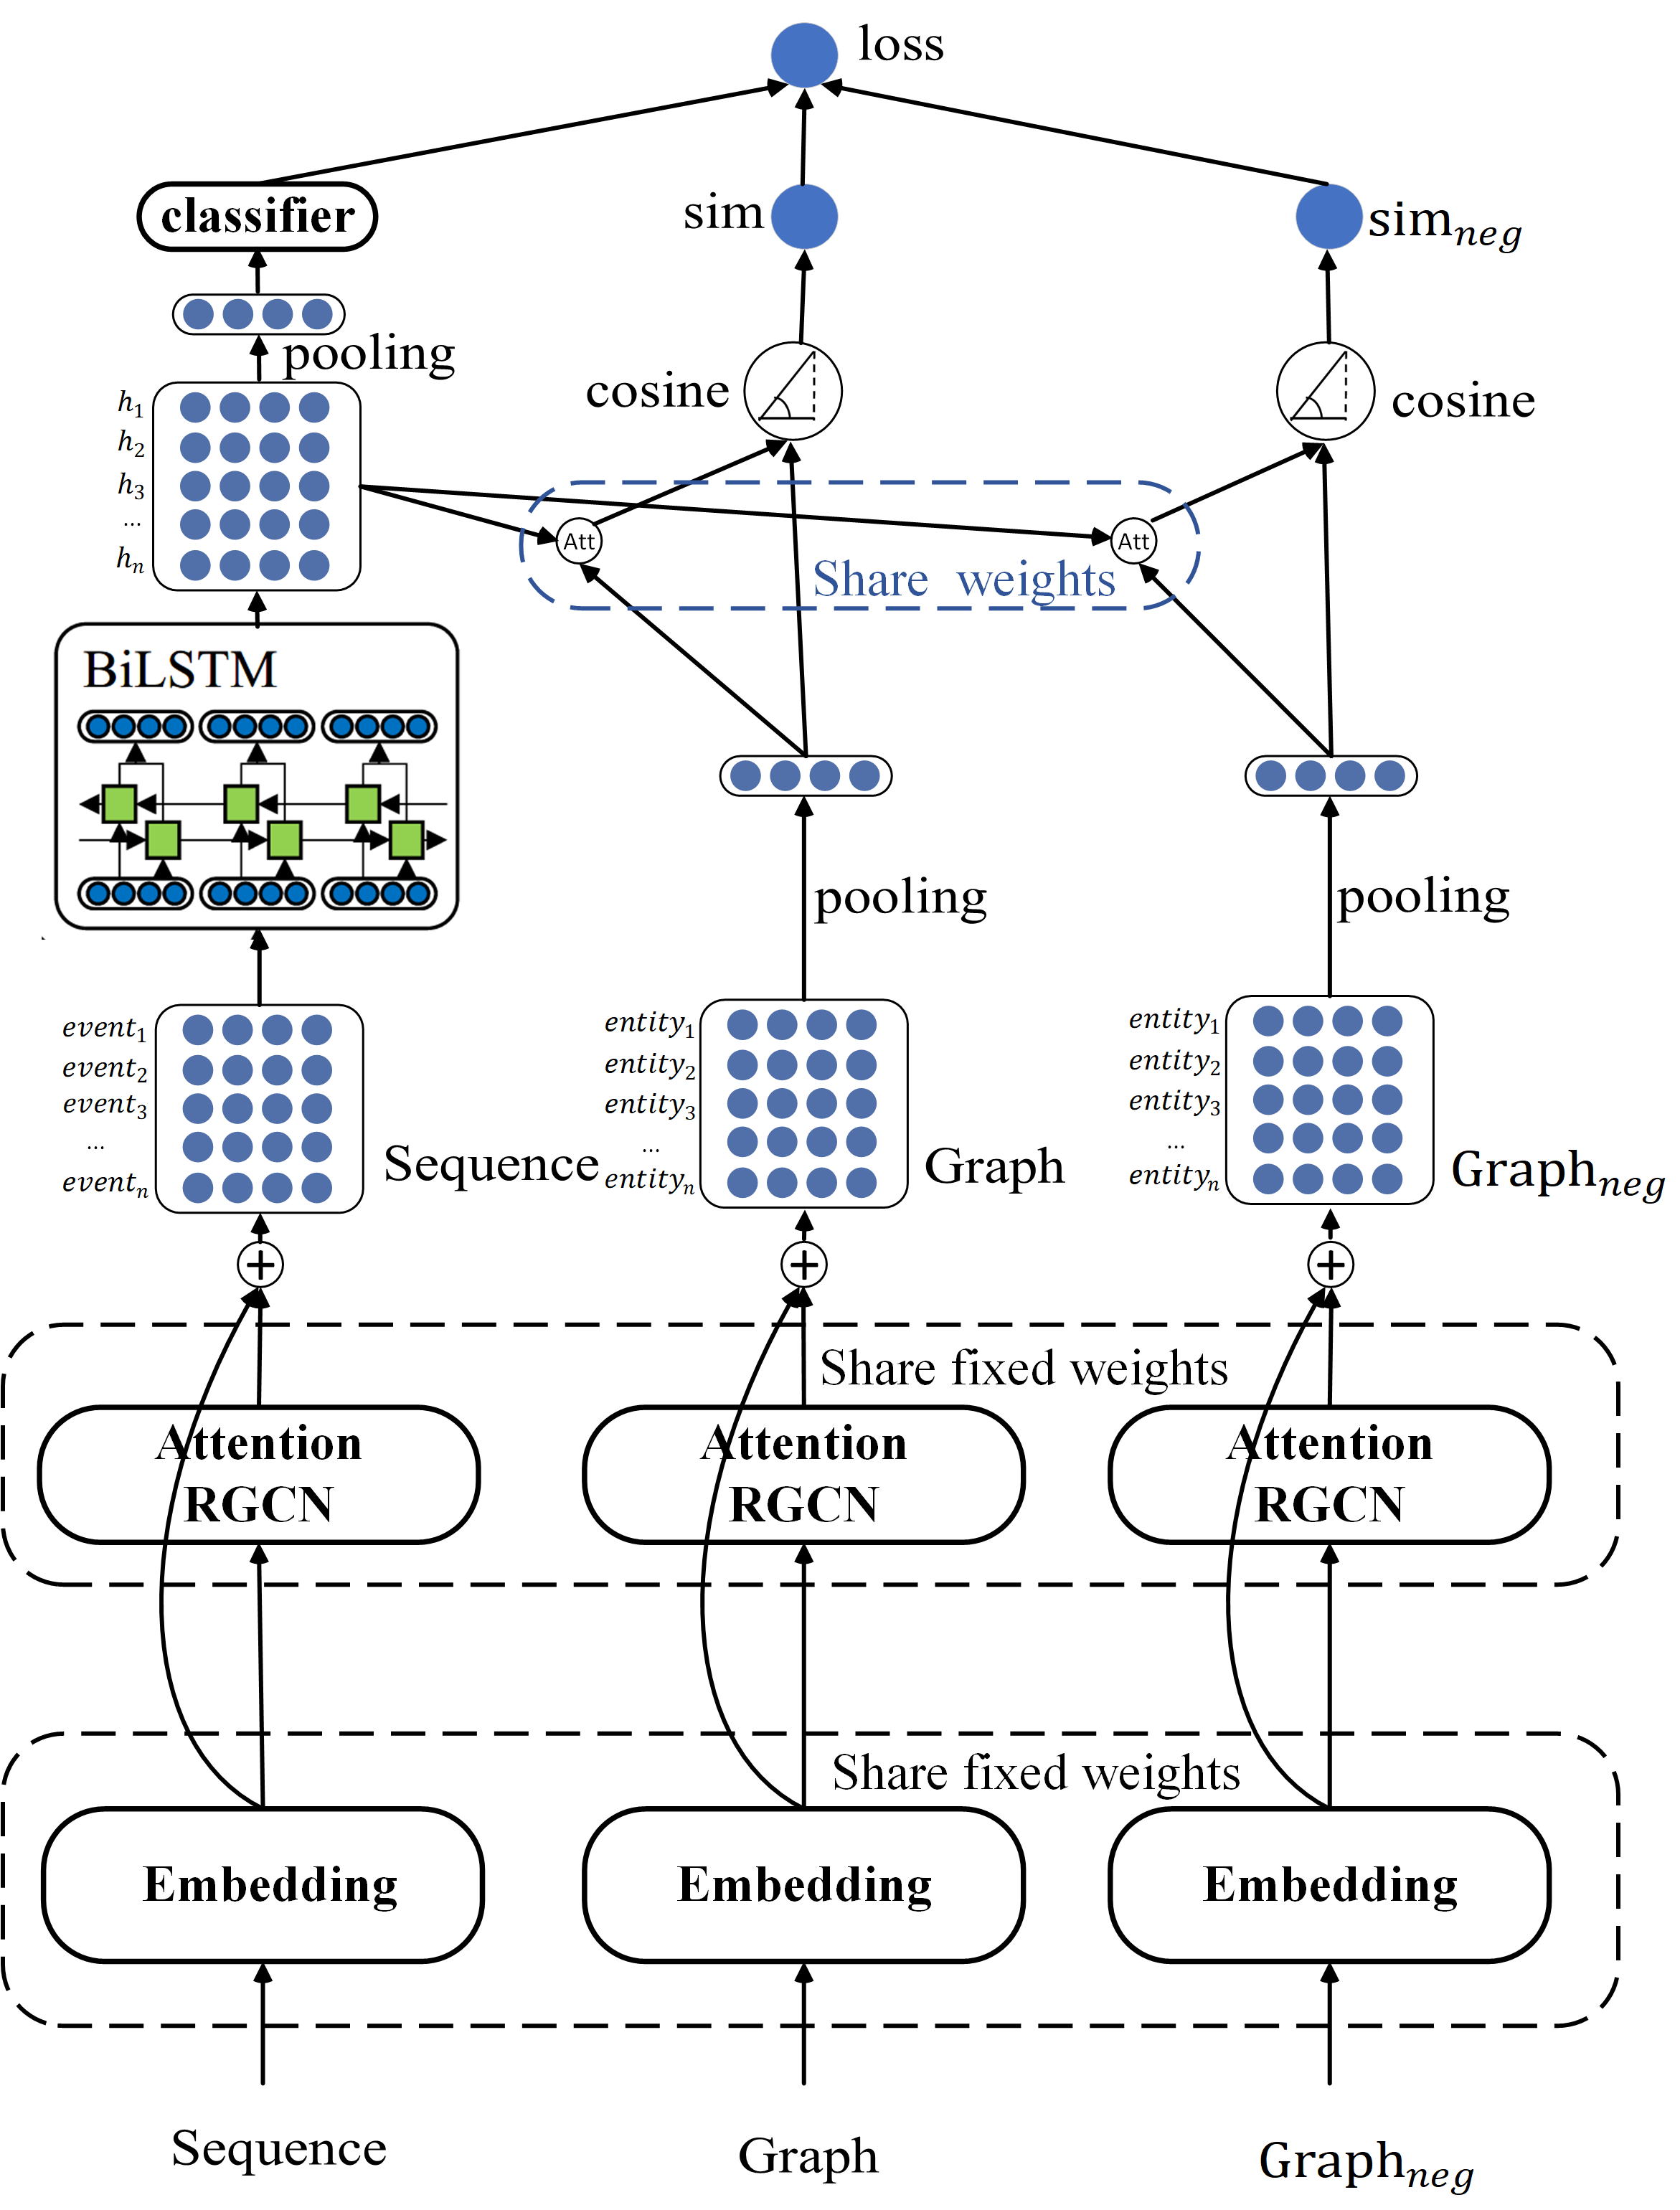
\includegraphics[width=.6\textwidth]{predict-error-model.png}
    \caption{故障预测模型\label{predict-error-model}}
\end{figure}
图\ref{predict-error-model}是引入组件-事件知识图谱的故障预测模型。其中嵌入层、Attention-RGCN使用组件-事件知识图谱表示学习模型的结构与参数,并固定不变。双向记忆网络使用上一小节的模型,参数后续进行训练学习。注意力层和分类层的参数也会在后续进行学习。

嵌入层规定了实时事件序列和知识图谱的嵌入方式。图\ref{input-event-sequence}为一个实时事件序列案例,可见实时事件序列中每个事件也都对应着所在的组件,且组件之间存在着拓扑关系,只是每个组件都有其唯一标识,但对应的组件类型未发生改变,所以同样可以使用图\ref{kg-representation}中的表示学习模型,获取每个实时事件的嵌入表示向量。组件-事件知识图谱则同图\ref{graph-example}所示。输入层中的embedding和Attention-RGCN均使用章节\ref{representation-paras-learn}所学到的参数并固定,实时事件序列和组件-事件知识图谱都会共享这些参数用于嵌入表示。
\begin{figure}[htbp]
    \centering
    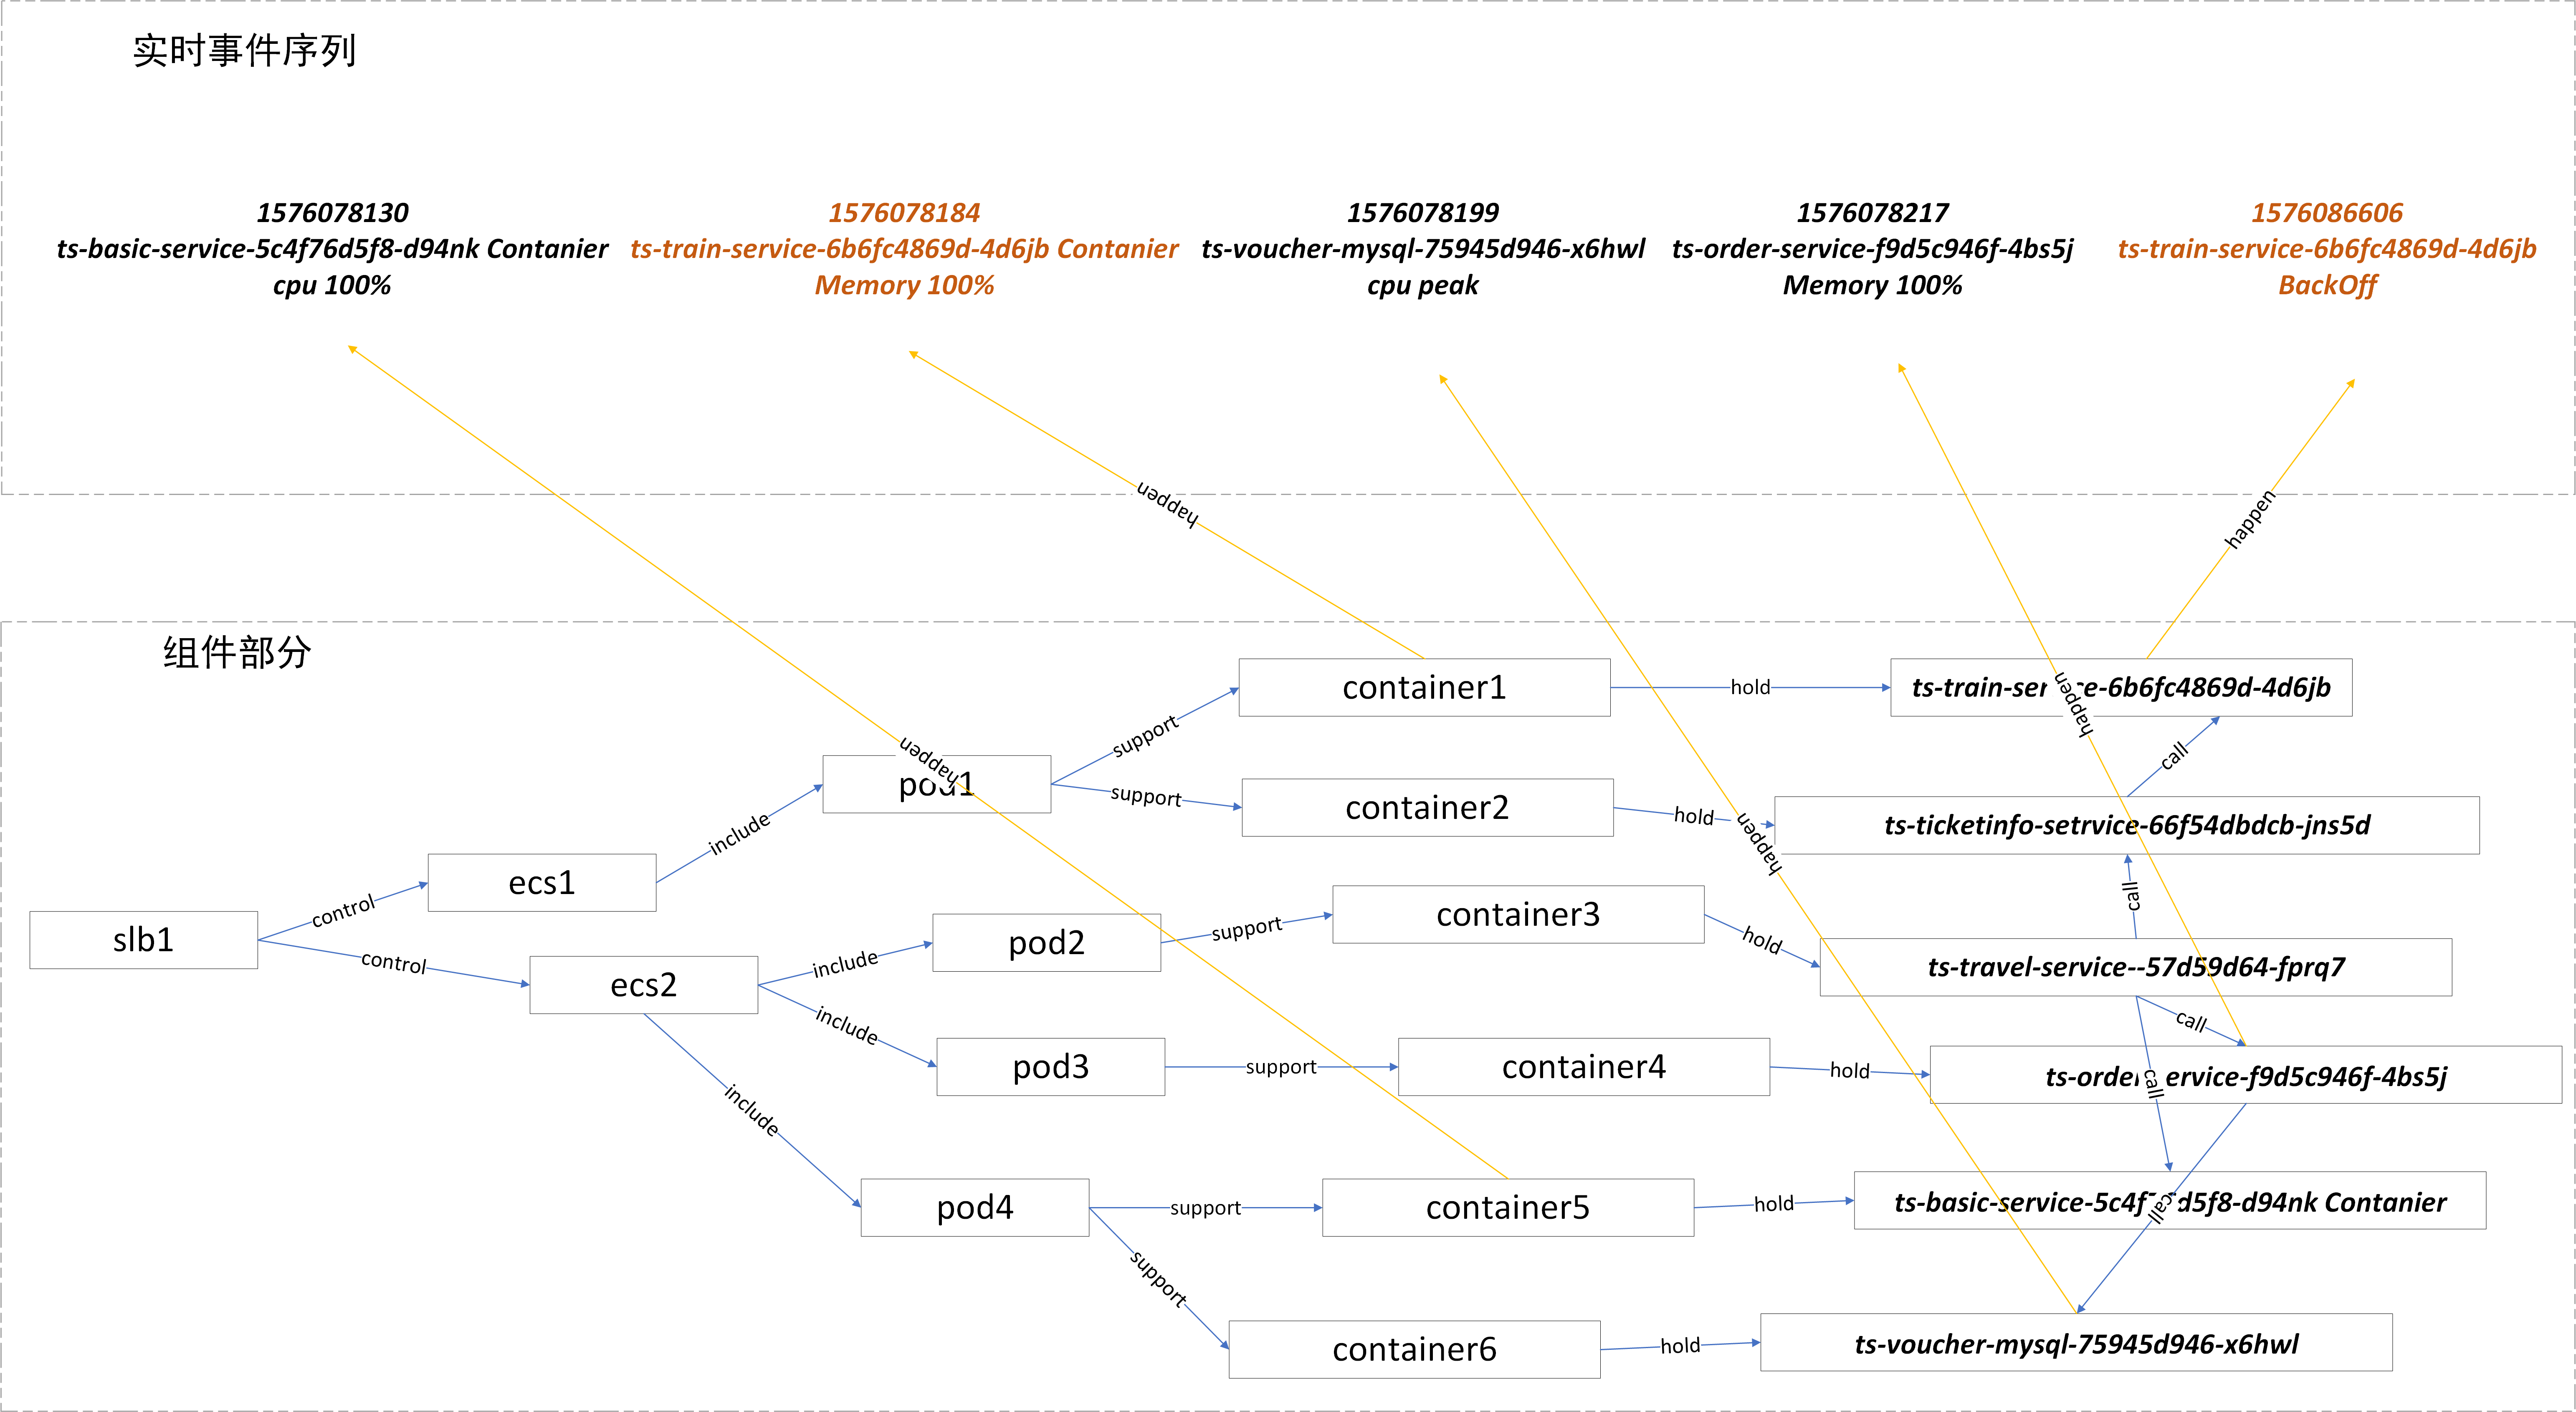
\includegraphics[width=.9\textwidth]{input-event-sequence.png}
    \caption{输入实时事件序列样例\label{input-event-sequence}}
\end{figure}

双向记忆网络层用来获取实时事件序列之间的时序特征。在实时事件序列中,虽然存在着组件之间的拓扑关系,但不存在事件之间的因果关系,事件之间只存在着前后的时序信息。记忆网络层使用上节\ref{memory-net-section}中的双向记忆网络模型,该模型已经在已有的故障预测工作中取得了最佳的效果。

在注意力层中,特定故障类型的组件-事件知识图谱会对经过双向记忆网络得到的隐状态序列做注意力权重累加。这样的注意力计算方式可以让知识图谱选择其所关注的事件子序列,并减少了噪声事件的干扰。输入事件序列$X=\left\{x_{1}, x_{2} \ldots x_{m}\right\}$在经过嵌入层和双向记忆网络后会得到隐向量序列$\left\{h_{1}, h_{2} \ldots h_{m}\right\}$。如式\ref{sequence-hidden}所示,注意层会首先计算知识图谱对隐状态序列的权重$\alpha_{(. , g)}$,然后进行权重累加获取事件序列嵌入表示$h_{sequence}$。

\begin{equation}
    \begin{array}{l}
    e_{(h_{i} , g)} = h_{i}\mathbf{W}g\\
    \alpha_{(h_{i} , g)}=\operatorname{softmax}\left(e_{(h_{i} , g)}\right)=\frac{\exp \left(e_{(h_{i} , g)}\right)}{\sum_{j=0}^{m}  \exp \left(e_{\left(h_{j} , g\right )}\right)}\\
    h_{sequence} = \sum_{i=0}^{m}\alpha_{(h_{i} , g)}\cdot h_{i}\\
    \end{array}
    \label{sequence-hidden}
\end{equation}

输出层分为两方面,一方面会将双向记忆网络的输出平均池化后得到的向量直接进行预测分类(有无故障),另一方面将组件-事件知识图谱的嵌入表示与注意力层权重累加得到的序列嵌入表示$h_{sequence}$做相似度计算,输出每张故障类型对应组件-事件知识图谱的相似度得分,按得分从高至低排列,即可得到预测故障类型排列结果。

\subsection{参数学习}
模型的损失函数如式\ref{graph-sequence-predict}所示,分为两部分。在预测判别有无故障时,使用基于交叉熵的损失函数。在知识图谱相似匹配时,通过负采样用边际损失作为损失函数。
\begin{equation}
    \begin{aligned}
        \mathcal{L}=-\sum_{i=1}^{n}[Y_{i} \log \left(f\left(X_{i} \right)\right)
        +\left(1-Y_{i}\right) \log \left(1-f\left(X_{i} \right)\right)\\
+Y_{i}\cdot \max \left (0, \cos \left (h_{i}, g_{neg} \right ) - \cos \left (h_{i}, g \right )\right )]
    \end{aligned}
    \label{graph-sequence-predict}
\end{equation}

其中,$X_{i}$为第$i$个输入事件序列$\left\{x_{1}, x_{2} \ldots x_{m}\right\}$,$Y_{i}$为第$i$个输入事件序列有无故障的标签(0表示输入事件序列无故障,1表示输入事件序列有故障)。$h_{i}$为$X_{i}$事件序列的隐状态嵌入表示,$g$为$X_{i}$对应故障类型的组件-事件知识图谱的嵌入表示,$g_{neg}$为负采样任意一个与$X_{i}$不匹配的组件-事件知识图谱的嵌入表示向量。

\section{本章小结}
本章主要介绍了基于实时事件序列和组件-事件知识图谱的故障预测,通过上一章的组件-事件知识图谱表示学习模型获取每个故障类型对应的组件-事件知识图谱的嵌入表示向量,然后对双向记忆网络编码的实时事件序列隐状态进行注意力权重累加获取事件序列嵌入表示,最后计算两个嵌入表示向量的相似度,按照相似度从高至低排序即可得到预测的故障类型列表。本文的故障预测模型可以具体到故障类型,同时引入组件-事件知识图谱进行注意力计算,使得预测结果具有了可解释性。
\chapter{基于知识图谱的IT运维辅助系统设计与实现}
实时运行的集群中存在着大量的组件与实时数据,IT运维人员面对海量的信息需要消耗大量精力和时间逐步查询分析多源的繁杂数据。一个基于知识图谱的IT运维辅助系统可以有效地辅助运维人员,帮助其及时发现集群异常并预测可能出现的故障,从而大大降低了运维难度。

本章基于第三章、第四章和第五章提出的各个方法模型,设计并实现了一个基于知识图谱的IT运维辅助系统,并对设计与实现过程展开了细致地描述。本章共分4小节来介绍系统,介绍的内容包括需求分析、系统总体设计、系统详细实现和系统测试。
% 本文设计实现的系统通过jaeger\cite{mengistu2020distributed}、prometheus\cite{padgham2002prometheus}、阿里云公开API等方式获取集群拓扑结构、微服务间拓扑结构、日志数据和指标时序数据,将集群实时运行状态可视化。随后,历史监测数据被按故障类型分组,经过事件因果关系挖掘模型构建了每种故障对应的组件-事件知识图谱。基于构建的组件-事件知识图谱,利用上文提出的表示学习模型和故障预测模型,本系统可以根据实时发生的事件序列预测可能会发生的故障,提醒运维人员及时采取应对措施。


\section{需求分析}\label{need-analysis}
本节详细介绍基于知识图谱的IT运维辅助系统需要满足的需求,包括功能性需求和非功能性需求。功能性需求是指IT运维辅助系统要实现的功能,而非功能性需求是指该系统应当满足的除功能性需求之外的其他需求。
\subsection{功能性需求}
本系统主要目的是辅助IT运维人员,降低实际运维的难度。因此,在系统实现前,本文咨询了IT运维人员,进行了详细的需求调研,总结了IT运维辅助系统的三大功能需求:实时集群状态查询、组件-事件知识图谱查询及调优、实时故障预测。图\ref{user-need}为本章IT运维辅助系统用例图。
\begin{figure}[htbp]
    \centering
    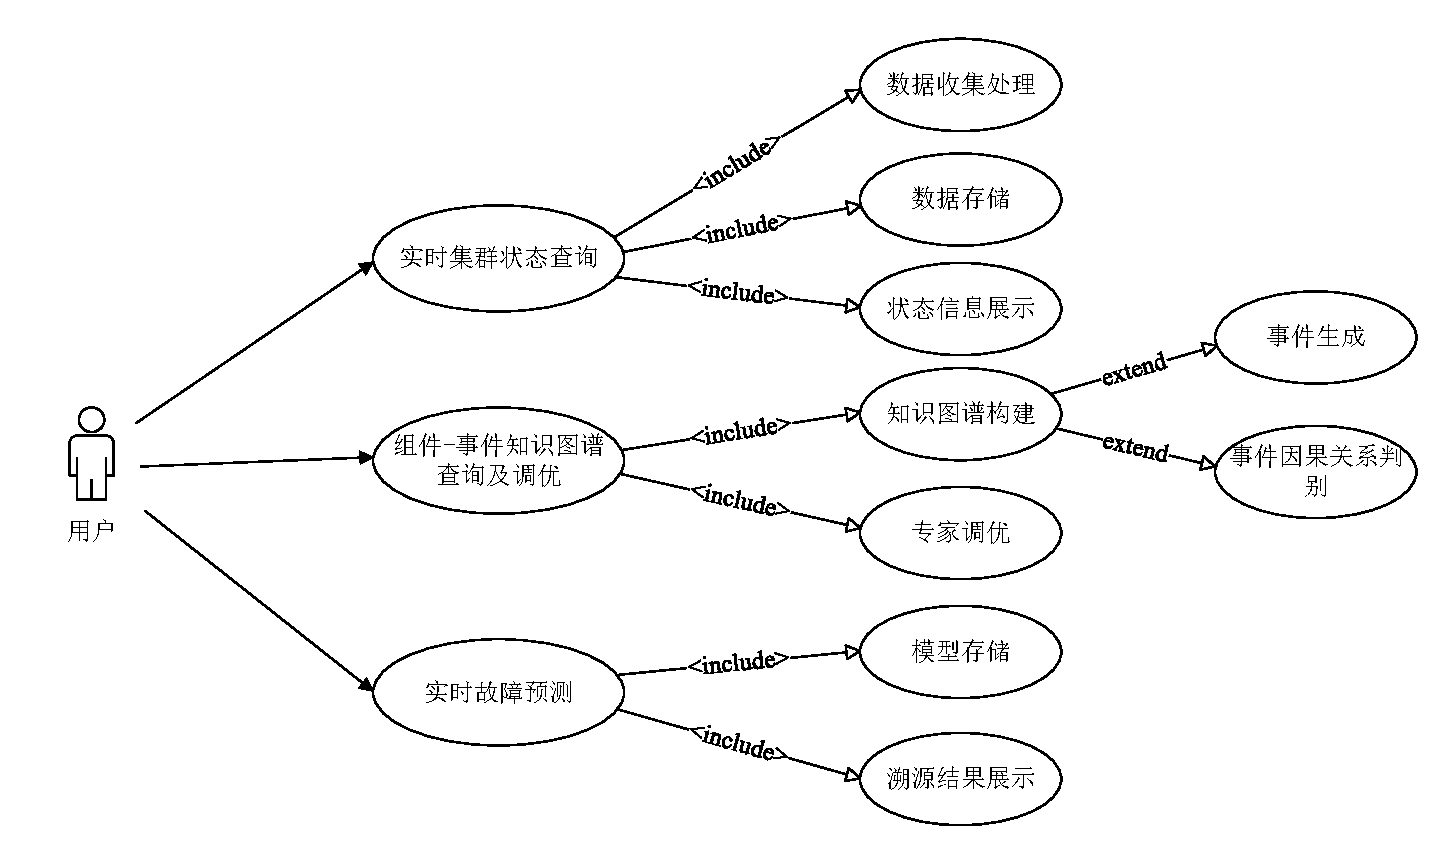
\includegraphics[width=0.98\textwidth]{user-need.pdf}
    \caption{IT运维辅助系统用例图\label{user-need}}
\end{figure}

(1)实时集群状态查询

分布式集群往往包含着上千个组件,每个组件有其特异的属性信息。另外,每个组件会实时产生不同种类的信息:硬件组件会产生内存、读写、CPU 等时序数据,软件组件会产生文本类的日志数据。在分布式集群实际运转时,每秒钟会产生万级的多源异构数据。

IT运维人员在实际工作中,需要调用不同接口,使用不同的开源软件才能全方面的了解每个组件的状态。繁琐的集群状态查询过程,不仅消耗了IT运维人员大量的精力,还会导致运维人员错失最佳的故障解决时机。因此,IT运维人员需要一个能够全面便捷地获取系统状态信息的查询系统。这个集群状态查询系统需要整合多个接口,收集各种状态数据,并将这些数据存储起来。另外,该系统需要提供简洁的查询界面,方便IT运维人员直观地操作。

(2)组件-事件知识图谱查询及调优

组件-事件知识图谱直观地展示了故障触发过程,包含着丰富的运维知识。运维人员在实际工作时,需要查询这些知识图谱,获取运维知识,指导下一步运维工作。系统需要根据第三章的组件-事件知识图谱构建流程,在后台从历史数据沉淀出组件-事件知识图谱。在知识图谱构建时,需要将多源异构数据转为统一规范的事件类型数据,并调用分类器获取事件间因果关系。这种依靠机器学习构建组件-事件知识图谱的方式,虽然能够快速沉淀出可用的故障触发知识,但始终不能做到完全精准,需要运维人员介入,进行少量的人工调优。基于以上分析,本系统需要构建并展示组件-事件知识图谱,方便IT运维人员查询,也方便其对知识图谱进行验证与调优。

(3)实时故障预测

在实际运维工作中,运维人员很难预知是否会有故障发生,往往是在故障发生后采取修复工作。这样解决已发生故障的工作模式,很难避免故障带来的损失。因此,本系统需要提供实时故障预测的功能,能够结合组件-事件知识图谱和实时的运行状态数据,给出准确具体的故障预测结果。为了实现实时故障预测,本系统需要存储多个模型,并给出故障预测结果的可视化展示。


\subsection{非功能性需求}
IT运维辅助系统除了需要满足上节所提的功能,还要满足以下非功能需求:

% (1)故障预测结果要具体准确,系统除了要预测是否会出现故障,还要给出具体会出现的故障,并且预测结果准确率要高。
(1)各个查询接口返回结果要迅速,需要在2s内给出查询结果。

(2)故障预测过程要迅速,系统需要根据实时产生的数据,在5s的响应时间内给出正确预测结果。


\section{系统总体设计}
本节进行了系统的总体设计,首先给出了系统的总体框架图,随后介绍了各个功能模块的设计。
\subsection{系统总体框架图}
本系统使用B/S(Browser/Server)架构,即用户使用浏览器请求服务,后台服务器响应返回结果的工作模式。B/S整体架构分为三个层次,包括模型、视图和控制器。其中,模型负责实现业务功能逻辑,即按照功能需求整合转换数据形式;视图则将数据可视化,即把模型返回的数据直观地易于理解地展示出来;控制器则是从视图中接收用户输入的数据,并将数据传送给模型。另外,按照系统功能又可以把系统结构划分为数据层、业务逻辑层和交互层。图\ref{system-constructure}展示了这三层结构。
% \begin{itemize}
%     \item [(1)]数据层。本系统的数据层主要用于存储各种数据,使用了三种存储数据库,用于存储不同类型的数据。Kafka用于缓存大量的微服务实时访问请求,这部分数据会被用于生成微服务间拓扑关系;Neo4j用于存储生成的组件-事件知识图谱;阿里云SLS用于存储日志数据和指标时序数据。
%     % 包含了日志数据、指标时序数据、集群组件拓扑和微服务间拓扑。这四类数据有不同的获取方式,具体获取方式在小节\ref{data-collect-way}进行了具体描述。
%     \item [(2)]业务逻辑层。业务逻辑层连接了数据层与交互层,包含了算法模型和业务逻辑。该层由多个模块协同工作实现系统功能,分为状态监测模块、组件-事件知识图谱构建模块和故障预测模块。每个模块的具体功能在下面几小节展开介绍。
%     \item [(3)]交互层。交互层将业务逻辑层数据可视化地直观展示在前端页面,并支持用户操作数据。本系统交互层主要分为三部分:组件-事件知识图谱查询及调优页面、实时集群状态查询页面和故障预测页面。
% \end{itemize}

(1)数据层。本系统的数据层主要用于存储各种数据,使用了三种存储数据库,用于存储不同类型的数据。Kafka用于缓存大量的微服务实时访问请求,这部分数据会被用于生成微服务间拓扑关系;Neo4j用于存储生成的组件-事件知识图谱;阿里云SLS用于存储日志数据和指标时序数据。

    % 包含了日志数据、指标时序数据、集群组件拓扑和微服务间拓扑。这四类数据有不同的获取方式,具体获取方式在小节\ref{data-collect-way}进行了具体描述。
(2)业务逻辑层。业务逻辑层连接了数据层与交互层,包含了算法模型和业务逻辑。该层由多个模块协同工作实现系统功能,分为状态监测模块、组件-事件知识图谱构建模块和故障预测模块。每个模块的具体功能在下面几小节展开介绍。

(3)交互层。交互层将业务逻辑层数据可视化地直观展示在前端页面,并支持用户操作数据。本系统交互层主要分为三部分:组件-事件知识图谱查询及调优页面、实时集群状态查询页面和故障预测页面。

\begin{figure}[htbp]
    \centering
    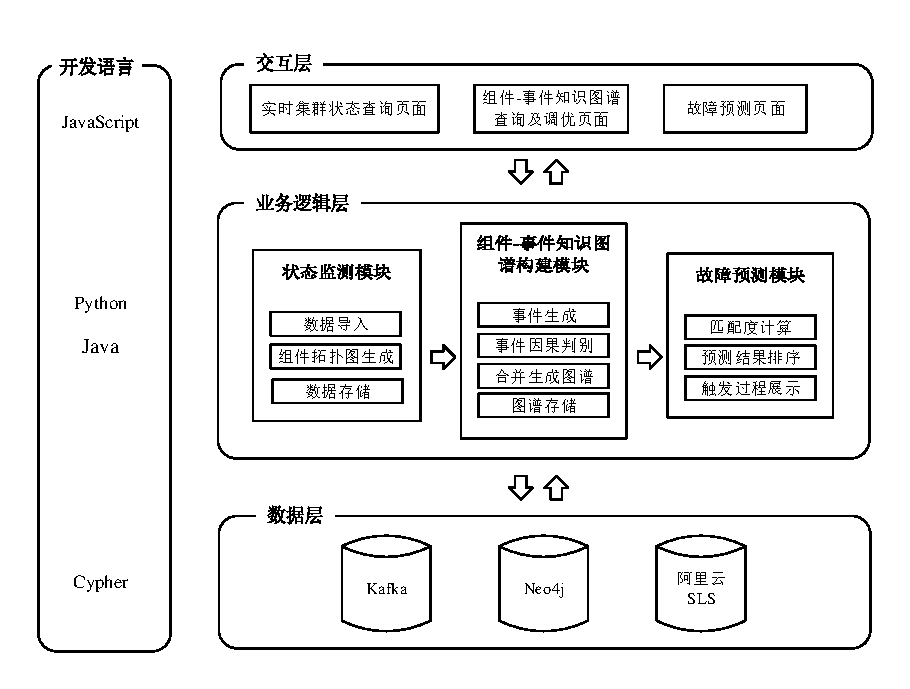
\includegraphics[width=0.8\textwidth]{system-constructure.pdf}
    \caption{IT运维辅助系统框架图\label{system-constructure}}
\end{figure}
% \begin{figure}[htbp]
%     \centering
%     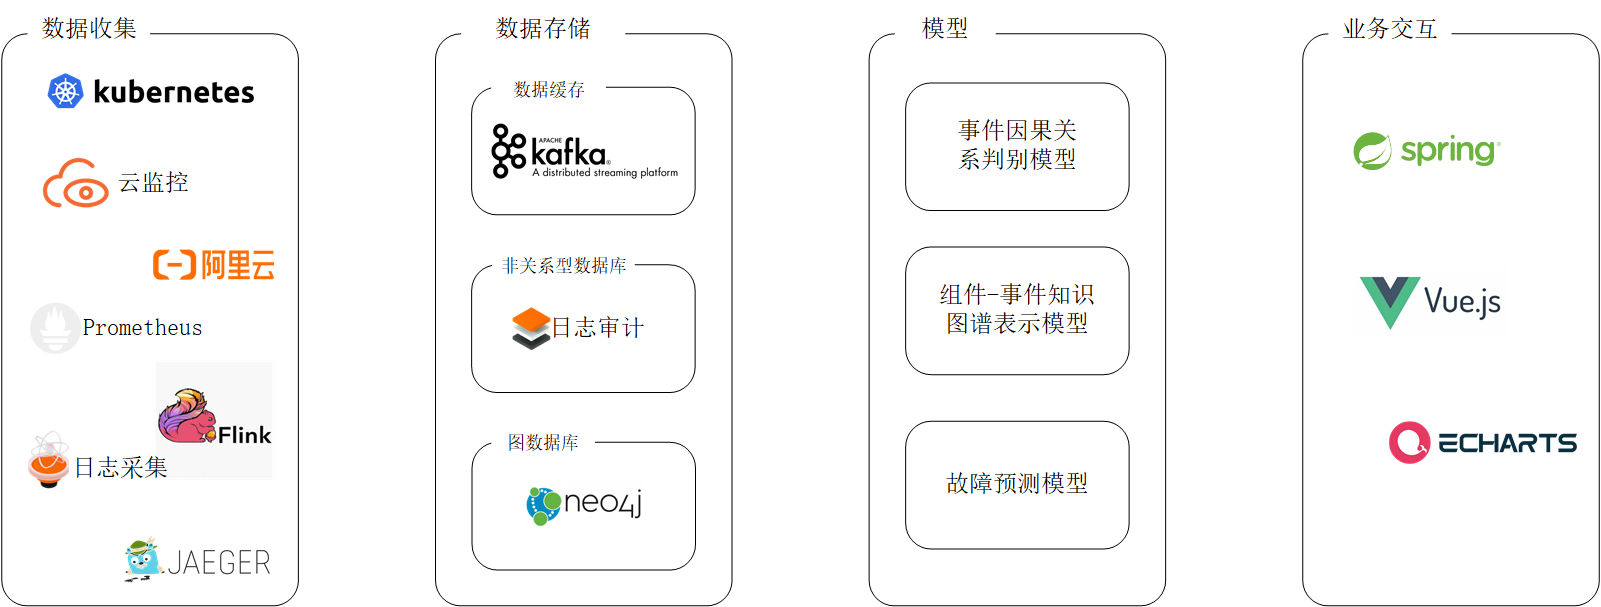
\includegraphics[width=0.8\textwidth]{system-technology.png}
%     \caption{IT运维辅助系统相关工具\label{system-technology}}
% \end{figure}

% \subsection{功能模块设计}\label{system-function}
\subsection{状态监测模块概要设计}
本模块主要负责将不同来源、不同种类的数据整合起来,减少IT运维人员查询数据的难度。该模块需要设计并实现数据导入、组件拓扑图生成和数据存储三部分,分别如下:
% \begin{itemize}
%     \item [(1)]数据导入部分要使用不同的API,不同的中间件,获取不同种类的数据,包括日志数据、指标时序数据、组件属性数据、微服务请求数据;
%     \item [(2)]组件拓扑图生成部分需要分析组件属性、微服务请求数据,生成组件间拓扑图;
%     \item [(3)]数据存储部分负责数据持久化,需要整理不同形式的数据,并根据数据特性存入不同的数据库中。
% \end{itemize}

(1)数据导入部分要使用不同的API,不同的中间件,获取不同种类的数据,包括日志数据、指标时序数据、组件属性数据、微服务请求数据;

(2)组件拓扑图生成部分需要分析组件属性、微服务请求数据,生成组件间拓扑图;

(3)数据存储部分负责数据持久化,需要整理不同形式的数据,并根据数据特性存入不同的数据库中。

\subsection{组件-事件知识图谱构建模块概要设计}
本模块的主要功能是从历史数据中沉淀生成组件-事件知识图谱。本模块需要设计并实现4个子功能:
% \begin{itemize}
%     \item [(1)]首先,该模块需要整理日志数据、指标时序数据,转化为统一格式的事件类型数据;
%     \item [(2)]随后,该模块需要调用机器学习模型,判别事件间是否有因果关系;
%     \item [(3)]然后,该模块需要合并生成的事件因果关系,生成抽象事件层图谱,再结合组件拓扑图得到组件-事件知识图谱;
%     \item [(4)]最后,该模块要把生成的组件-事件知识图谱存入Neo4j中,以保证可以被其他模块调用。
% \end{itemize}

(1)首先,该模块需要整理日志数据、指标时序数据,转化为统一格式的事件类型数据;

(2)随后,该模块需要调用机器学习模型,判别事件间是否有因果关系;

(3)然后,该模块需要合并生成的事件因果关系,生成抽象事件层图谱,再结合组件拓扑图得到组件-事件知识图谱;

(4)最后,该模块要把生成的组件-事件知识图谱存入Neo4j中,以保证可以被其他模块调用。

\subsection{故障预测模块概要设计}
本模块的主要功能是实时预测集群是否会发生故障,并给出故障预测结果排名。本模块需要设计并实现3个部分,分别为匹配度计算,预测结果排序和触发过程展示,具体如下:
% \begin{itemize}
%     \item [(1)]在匹配度计算部分,每个故障类型的组件-事件知识图谱,会分别与实时事件序列进行匹配度计算,匹配度越高意味着越有可能发生对应类型的故障。
%     \item [(2)]在预测结果排序部分,本模块会根据匹配度降序排列候选故障类型,当所有匹配度均小于阈值时,会认为不会有故障发生。
%     \item [(3)]在触发过程展示部分,本模块会结合组件-事件知识图谱和实时事件序列,给出可能会发生的故障的触发过程。
% \end{itemize}

(1)在匹配度计算部分,每个故障类型的组件-事件知识图谱,会分别与实时事件序列进行匹配度计算,匹配度越高意味着越有可能发生对应类型的故障。

(2)在预测结果排序部分,本模块会根据匹配度降序排列候选故障类型,当所有匹配度均小于阈值时,会认为不会有故障发生。

(3)在触发过程展示部分,本模块会结合组件-事件知识图谱和实时事件序列,给出可能会发生的故障的触发过程。

% 系统各功能模块已在图\ref{system-constructure}中业务逻辑层展示,分为:a.事件生成模块、b.组件拓扑生成模块、c.集群状态监测模块、d.事件因果判别模块、e.组件-事件知识图谱生成模块、f.故障预测模块。下面具体介绍这些模块的功能:
% \begin{itemize}
%     \item [a.]事件生成模块:收集各种实时的系统运行数据,将数据转化为统一规范的事件类型数据。
%     \item [b.]组件拓扑生成模块:分析集群组件属性信息列表,根据其中表明了集群组件关系的字段,生成集群组件拓扑。而微服务间的拓扑则利用其实际工作时的访问关系生成。
%     \item [c.]集群状态监测模块:根据事件发生所在的组件位置,将前两个模块数据关联起来,得到可视化的集群运行状态图。
%     \item [d.]事件因果关系判别模块:借助事件因果关系判别模型,分析事件间是否具有因果关系。
%     \item [e.]组件-事件知识图谱生成模块:从某类故障的历史数据中沉淀出包含组件依赖关系、组件事件产生关系和抽象事件因果关系的组件-事件知识图谱。
%     \item [f.]故障预测模块:基于集群状态监测模块所收集的事件序列,联合组件-事件知识图谱,预测未来可能发生的故障。
% \end{itemize}
\section{系统详细实现}
本节介绍系统的详细实现过程,分为3小节展开介绍,分别为状态监测模块详细实现、组件-事件知识图谱构建模块详细实现和故障预测模块详细实现。

\subsection{状态监测模块详细实现}\label{data-collect-way}
状态监测模块从多个源头获取多种类别的数据。本模块通过处理收集到的数据,生成共计4类数据,包括集群拓扑结构、微服务拓扑结构、日志数据、指标时序数据。下面分为4部分分别介绍这四种数据的实际收集、处理、存储流程。
% \subsubsection{集群拓扑结构}
% \begin{itemize}
    % \item [(1)]第一部分为集群拓扑结构数据。
    
    (1)第一部分为集群拓扑结构数据。
    
    首先,在系统开发时,引入阿里云提供的SDK核心库和组件的Maven项目依赖。其次,编写多线程代码调用不同组件的数据请求方法并设置参数,再保存方法返回的Json数据。如调用方法$DescribeImagesRequest(.)$,设置要查询的镜像类型$setImageOwnerAlias(.)$,就会返回对应镜像的Json格式的基本信息。
    
    随后,分析返回的Json数据,读取指定字段值。返回的Json数据不同字段包含着不同类型的信息,如字段$ ImageId: freebsd\_11\_02\_64\_30G\_alibase\_20190722.vhd$表明了镜像的唯一标识符;$OSNameEn: FreeBSD  11.2 64 bit$表明了系统名称;$VpcId:vpc—2zeuphj08tt7q3brd****$表明了ECS所在VPC。
    
    最后,按获取的字段信息构建实体属性列表,和组件间关联拓扑。

% \subsubsection{微服务拓扑结构}
    % \newpage
    % \item [(2)]第二部分为微服务拓扑结构的获取。
    \newpage
    (2)第二部分为微服务拓扑结构的获取。
    
    微服务依赖关系虽然在分布式应用的代码逻辑中已清晰规定,但应用的代码属于机密信息且阅读代码时耗过大。为了无需了解应用代码逻辑就可以获取微服务间访问拓扑关系,本系统选用开源Jaeger实时监控微服务间的访问信息,并存储到Kafka中。
    
    Jaeger获取微服务拓扑结构流程如图\ref{tracing-generate}所示,其中span的形状代表了它对应何种微服务。一个Span对应一条微服务被调用的记录,其记录了微服务被标识符为parentSpan中的微服务调用了一次。一个Trace对应着微服务间的一条请求链路。具体步骤如下:

    \begin{figure}[htbp]
        \centering
        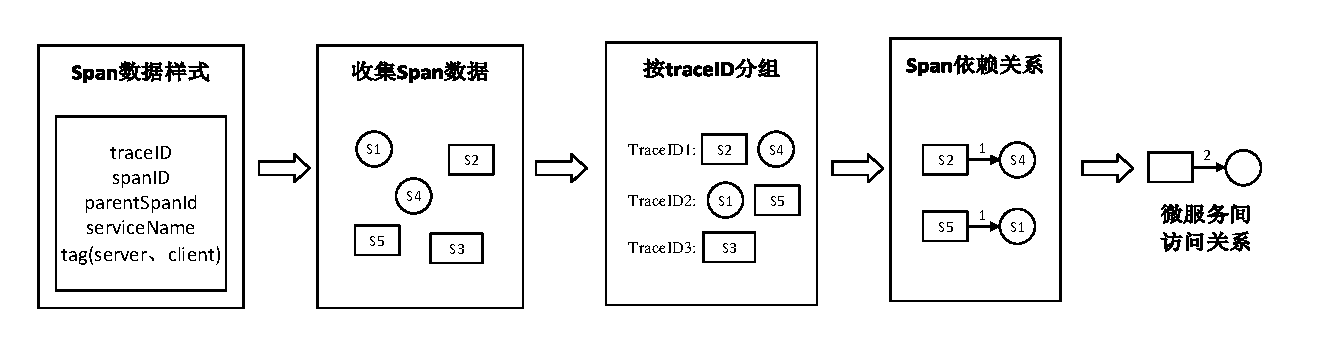
\includegraphics[width=0.9\textwidth]{tracing-generate.pdf}
        \caption{微服务间拓扑图生成流程\label{tracing-generate}}
    \end{figure}

    首先,获取Span数据,从Kafka中读取一个时间段内所有来源的Span。随后,分组Span数据,将所有Span按照traceID分组,这样就获得了traceID到Span集合的映射关系。然后,分析同组Span间依赖关系,即遍历每个Span对应的ParentSpanID,得到Span之间的父子依赖关系。其次,生成微服务间依赖关系,根据Span中serviceName信息,将Span间依赖关系映射为微服务间依赖关系。最后,生成微服务间拓扑图,将不同Trace中微服务间依赖关系整合规约,生成微服务拓扑图结构。

% \subsubsection{日志数据}
    % \item [(3)]第三部分为日志数据的收集。
    (3)第三部分为日志数据的收集。
    \begin{figure}[htbp]
        \centering
        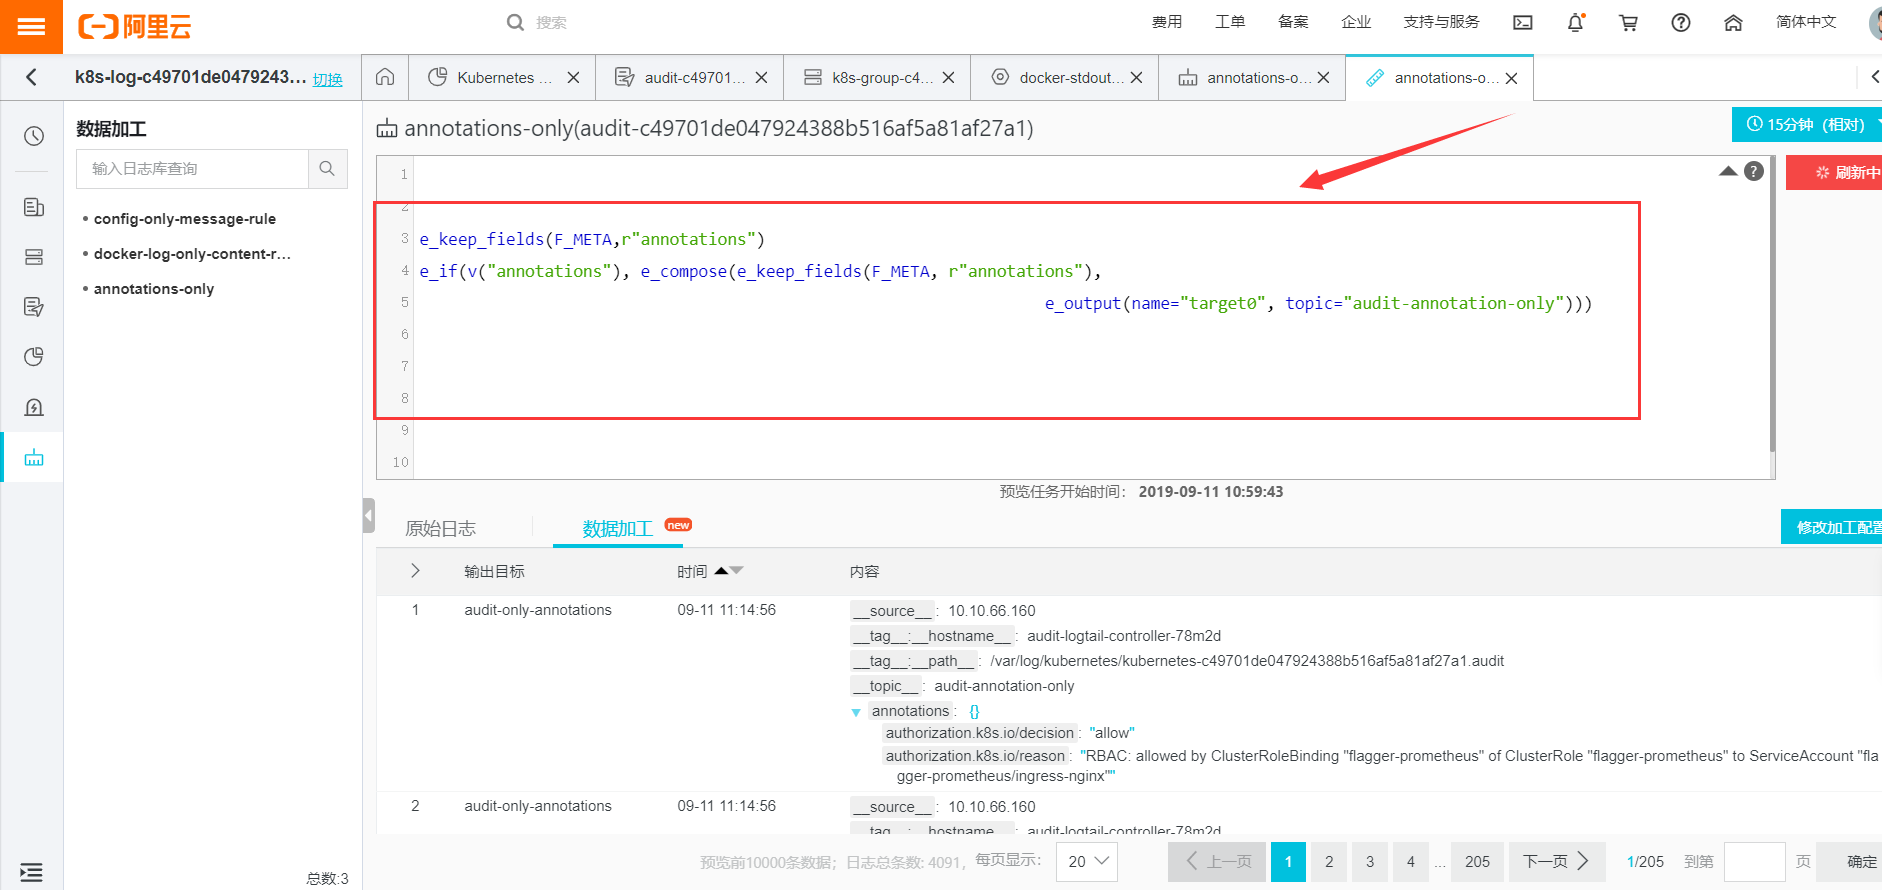
\includegraphics[width=0.9\textwidth]{data-process.png}
        \caption{数据加工指令示例\label{data-process}}
    \end{figure}

    首先对日志数据进行采集。阿里云日志服务(Log Service, SLS)提供了数据投递、查询、消费和采集等功能,可以高效的处理海量日志。在阿里云日志服务中创建Logstore,选择DockerIO、k8s日志等作为数据源,日志服务就会实时将数据汇总收集起来。

    然后,对日志数据进行加工。由于原始日志数据包含了很多无效信息,上一步得到的原始日志需要进一步加工处理只保留有效字段信息。加工过程直接使用日志服务的数据加工功能,编写加工命令选取保留的字段,并传输到新的Logstore中即可。如图\ref{data-process}所示图,该数据加工指令只保留了audit数据中的annotation字段。

    最后,使用公开API请求日志数据。经过上述步骤,日志数据被存储在日志服务各个Logstore中。当系统需要获取某段时间日志数据时,系统直接使用公开API并设置参数请求即可。如使用函数$PullLogsRequest(project, logStore, shardId, logNum, cursor)$并设置所要消费的project、LogStore和每次读取日志数量logNum等参数,就会返回符合参数约束的日志数据。

% \subsubsection{指标时序数据}
    % \item [(4)]第四部分为获取指标时序数据。
    (4)第四部分为获取指标时序数据。

    指标时序数据均为曲线类的数据,在存储形式上,均为一组时间戳到值的映射关系集合。其获取过程如下:首先,监测获取指标时序数据。在分布式集群中,多种组件都会有指标时序数据,且每个组件上会有不同种类的指标时序数据,如CPU、内存、磁盘吞吐率等。系统选用了Prometheus进行实时的监测。其次,对指标时序数据进行长期存储。由于Prometheus监测得到的指标时序数据不能长期存储(一般只保留14天),系统为了长期存储选择将数据导入日志服务。最后,使用公开API获取指标时序数据。将数据长期存储入日志服务平台后,系统可采用请求日志的API来请求获取指标时序数据。
% \end{itemize}

\subsection{组件-事件知识图谱构建模块详细实现}
本小节介绍构建组件-事件知识图谱的详细实现。在构建知识图谱之前,所有的历史故障数据都已按照故障类型进行了分组。在实际运行时,本模块接收用户的构建请求,根据对应的历史故障数据构建对应的组件-事件知识图谱,并返回构建结果。
% \begin{figure}[htbp]
%     \centering
%     
\includegraphics[width=0.8\textwidth]{request-construct.pdf}
%     \caption{构建组件-事件知识图谱请求样例\label{request-construct}}
% \end{figure}
% \ref{request-construct}

前端向后台发送的请求示例如下所示。请求URI路径为/construct,请求方式为POST,请求参数共包含两个字段。其中“faultType”表明了要构建哪个故障类型的知识图谱(当未设置时,默认构建所有故障类型的知识图谱),“showResult”表明是否展示构建结果。

\begin{lstlisting}[xleftmargin=12em,label=code]
    {
        "faultType": f3,
        "showResult": True
    }
\end{lstlisting}

在后台接收到请求后,本模块开始构建指定故障类型的组件-事件知识图谱,整个构建流程如图\ref{graph-constructure-process}所示。针对读取到的数据,本模块根据章节\ref{event-generate}中所述方法,对指标时序数据使用异常检测算法,对日志数据使用聚类算法,后续使用人工模板匹配转化为事件类型数据。对于生成的事件集合,按照时间先后顺序两两相连,得到候选因果关系集。为了加快对候选因果关系的判别,实际
开发中使用了多线程批量处理候选因果关系,直到候选因果关系集为空。每一个线程都调用事件因果关系判别模型,判别出真正存在的事件因果关系。所有被判别为存在的事件因果关系被收集了起来,规约生成抽象事件因果图。

最后,按照章节\ref{graph-generate}中的方法,本模块合并组件拓扑图和抽象事件因果图,生成对应故障类型的组件-事件知识图谱,并存入到Neo4j中。
\newpage
\begin{figure}[htbp]
    \centering
    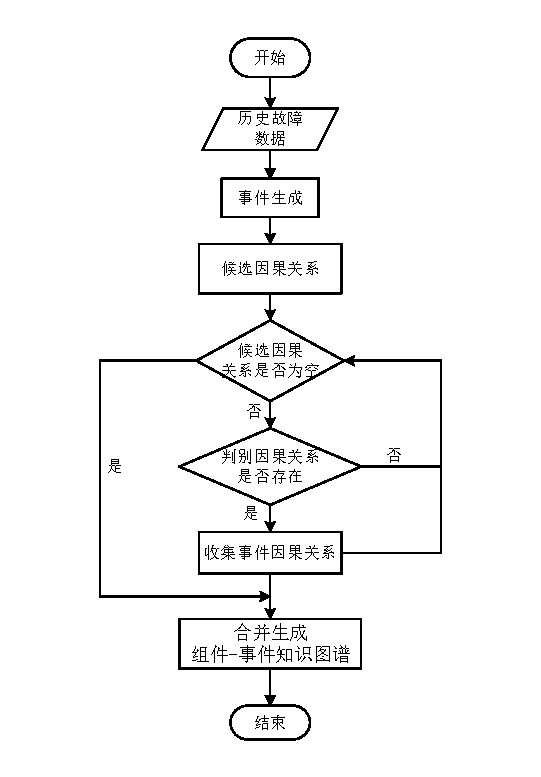
\includegraphics[width=0.6\textwidth]{graph-constructure-process.pdf}
    \caption{组件-事件知识图谱构建程序流程图\label{graph-constructure-process}}
\end{figure}

% \begin{figure}[hb]
%     \centering
%     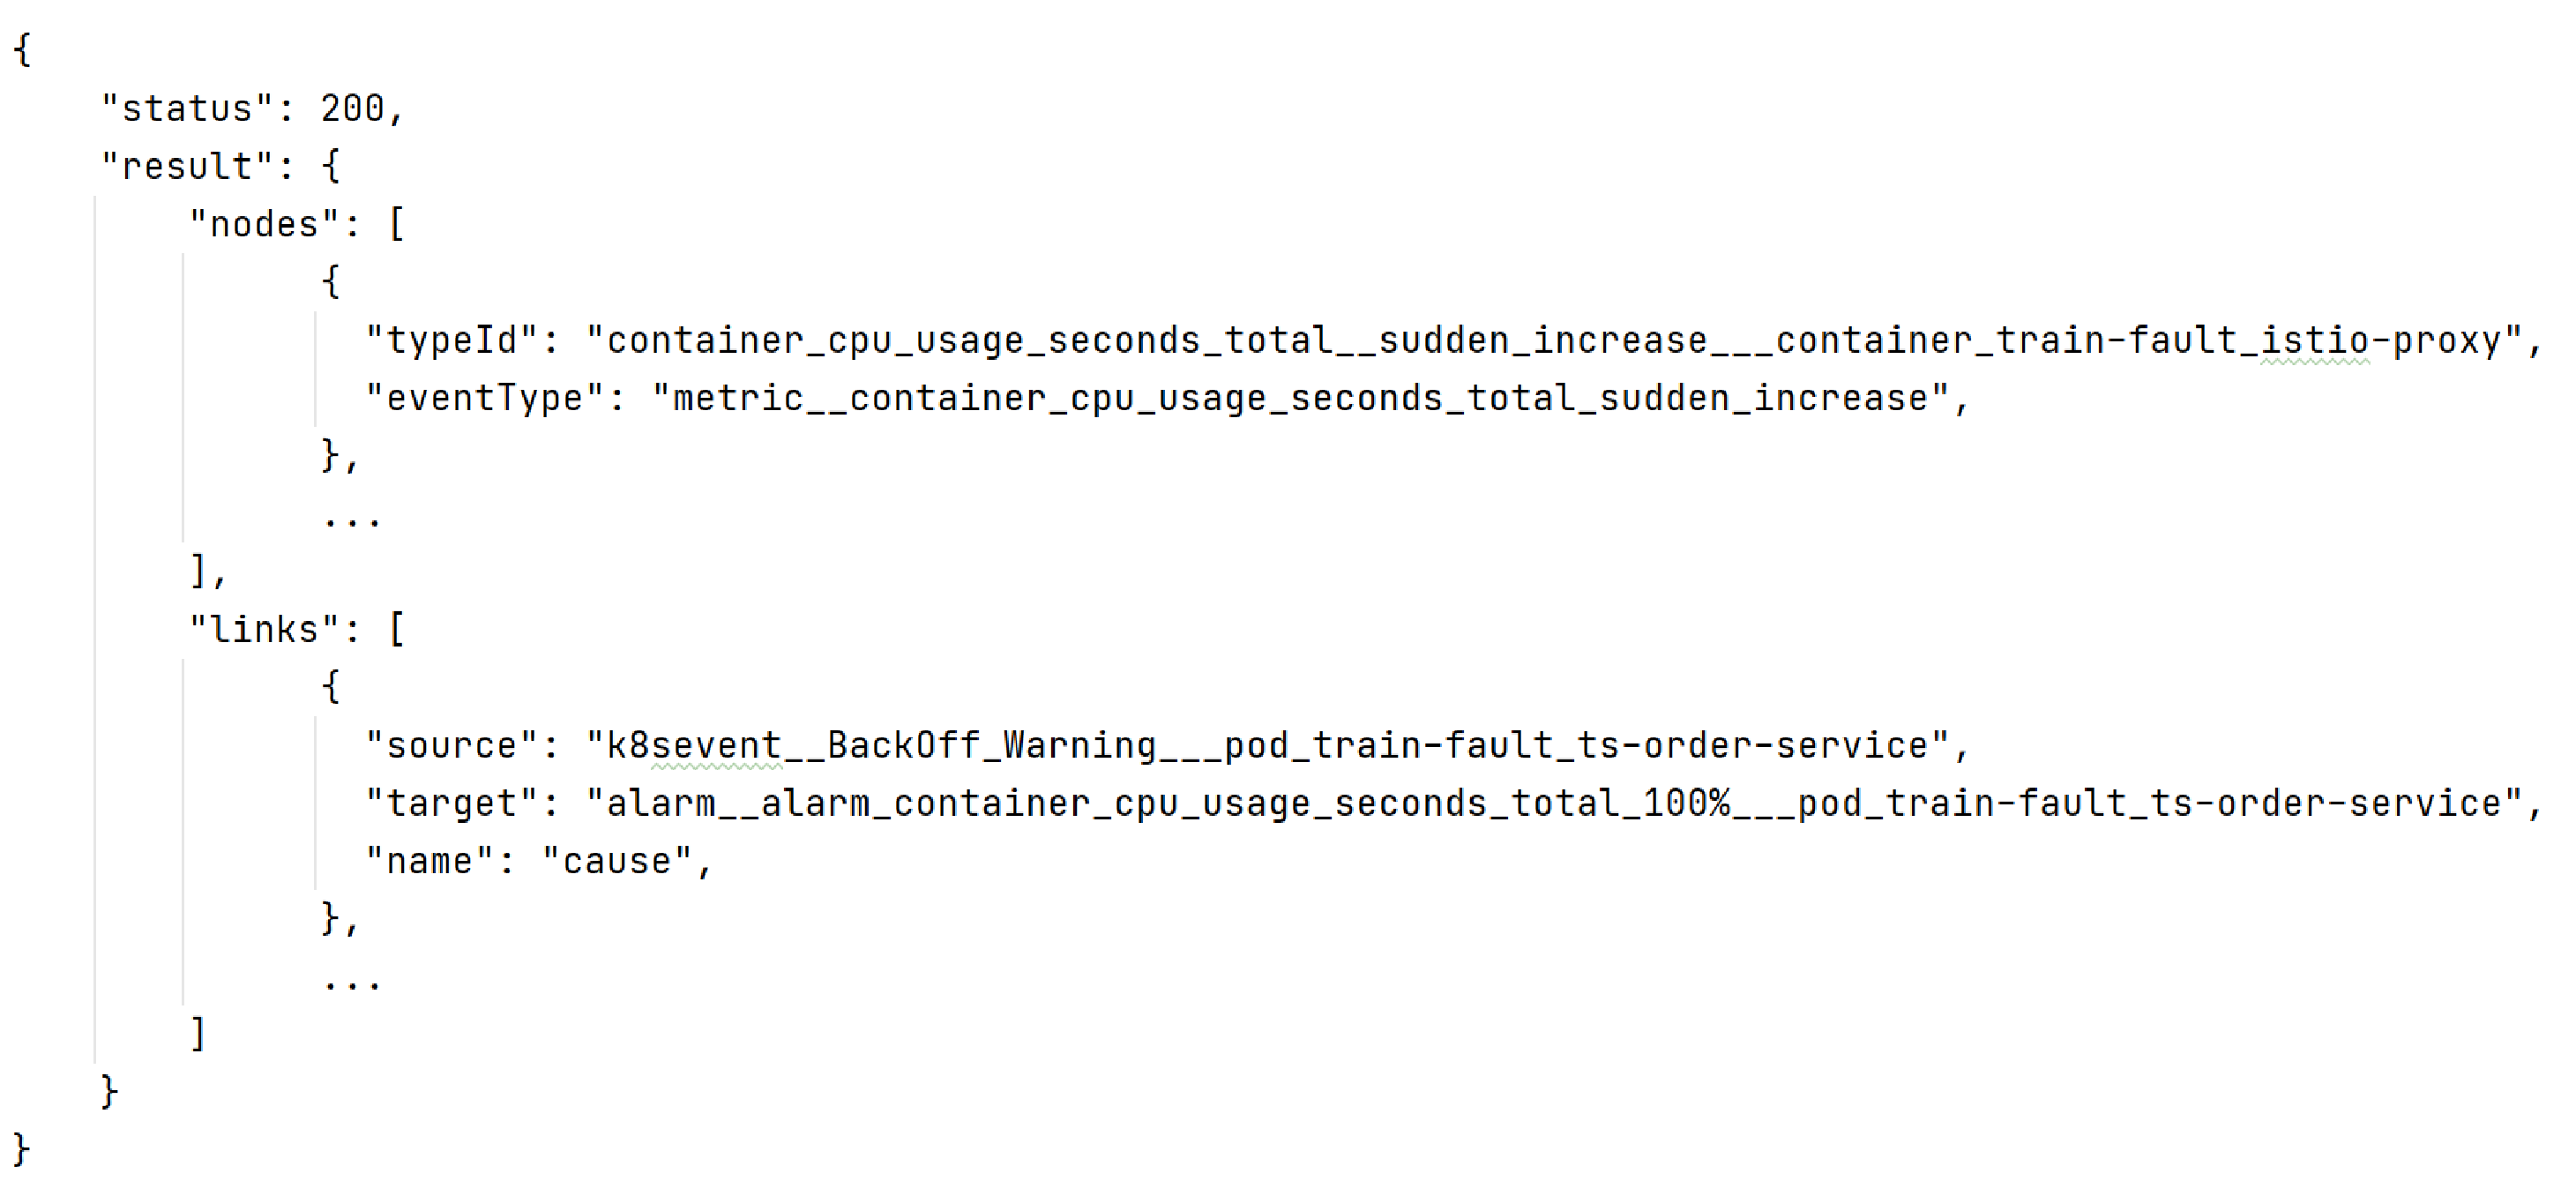
\includegraphics[width=0.8\textwidth,height=0.23\textheight]{construct-result.pdf}
%     \caption{构建组件-事件知识图谱响应样例\label{construct-result}}
% \end{figure}

另外,后台会向前端返回响应结果,如下所示。其中,“status”返回请求响应状态,“result”返回了所构建图谱的结点、关系列表。列表中详细记录着每个结点、每条关系的属性信息。
\begin{lstlisting}[xleftmargin=8em]
    {
        "status": 200,
        "result": {
            "nodes": [ 
                {
                    "typeId": "app_log__INFO_1_tracing...",
                    "eventType": "app_log__INFO_1",
                }...],
            "links": [...]
        }
    }
\end{lstlisting}

\subsection{故障预测模块详细实现}
本节介绍故障预测模块的详细实现过程。故障预测模块被启动后,其会默认一直运行,不停地监测实时事件序列,并给出故障预测结果。运维人员在不需要故障预测时,将该功能手动关闭即可。

\begin{lstlisting}[xleftmargin=2em]
    {
        "eventSequence": [
            {
                "id":"container_cpu_usage_seconds_total__sudden...",
                "time": "1576077300",
                "location": "container_train-fault_ts-verificat...",
                "event_type": "cpu_usage_seconds_total__sudden...",
                "detail": "2019-12-11 23:15:00/1576077300 pod...",
            }, 
            ...]
    }
\end{lstlisting}

每当状态监测模块监测到新事件后,就会向故障预测模块发送一个请求。请求URI路径为/failurePredict,请求方式为POST,请求参数中包含着最新的1024个事件(少于1024时,故障预测模块会补零)。请求示例如上所示,“eventSequence”字段记录着事件序列中每个事件的属性字典。
% \begin{figure}[htbp]
%     \centering
%     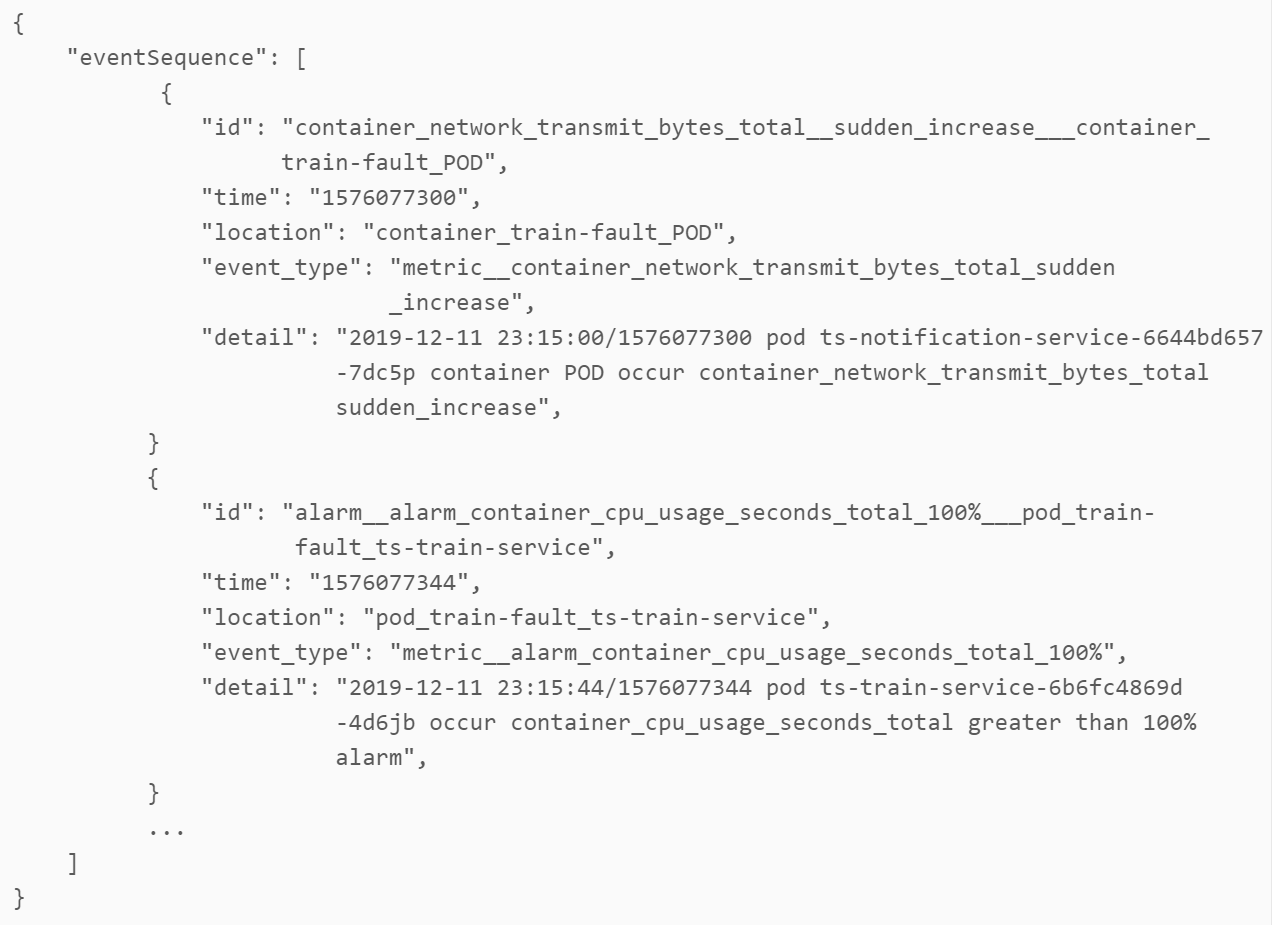
\includegraphics[width=0.8\textwidth]{predict-request.png}
%     \caption{故障预测请求样例\label{predict-request}}
% \end{figure}
% \ref{failure-predict-process}

\begin{figure}[H]
    \centering
    \center{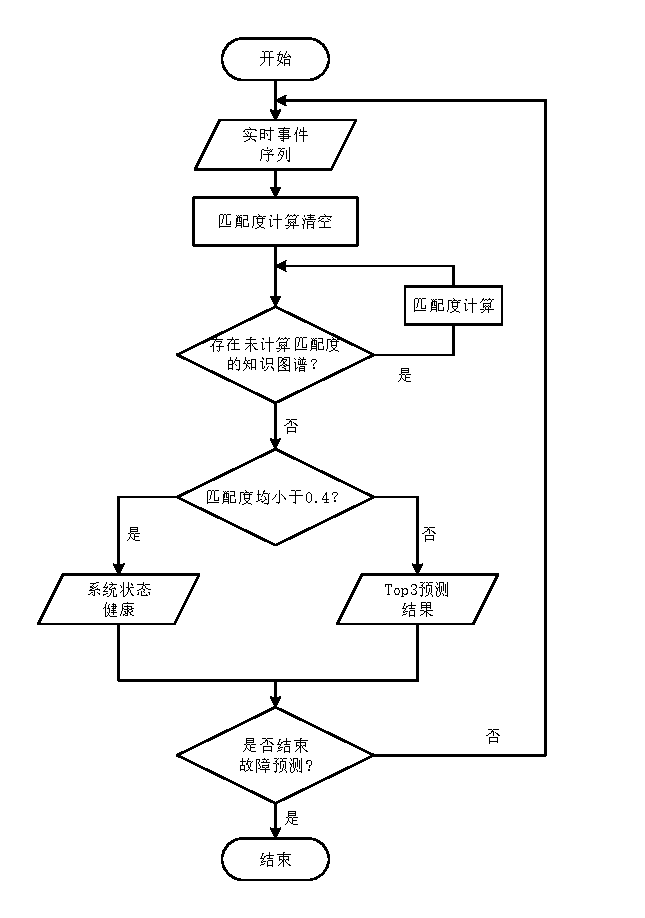
\includegraphics[width=0.65\textwidth,height=0.495\textheight]  {failure-predict-process.pdf}}
    % 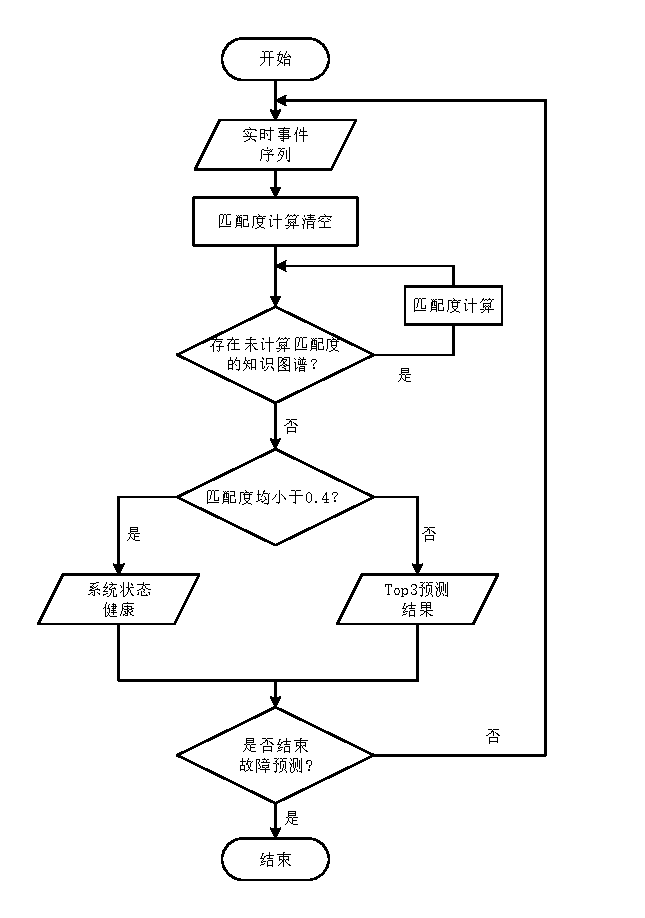
\includegraphics[width=0.65\textwidth,height=0.521\textheight]{failure-predict-process.pdf}
    % 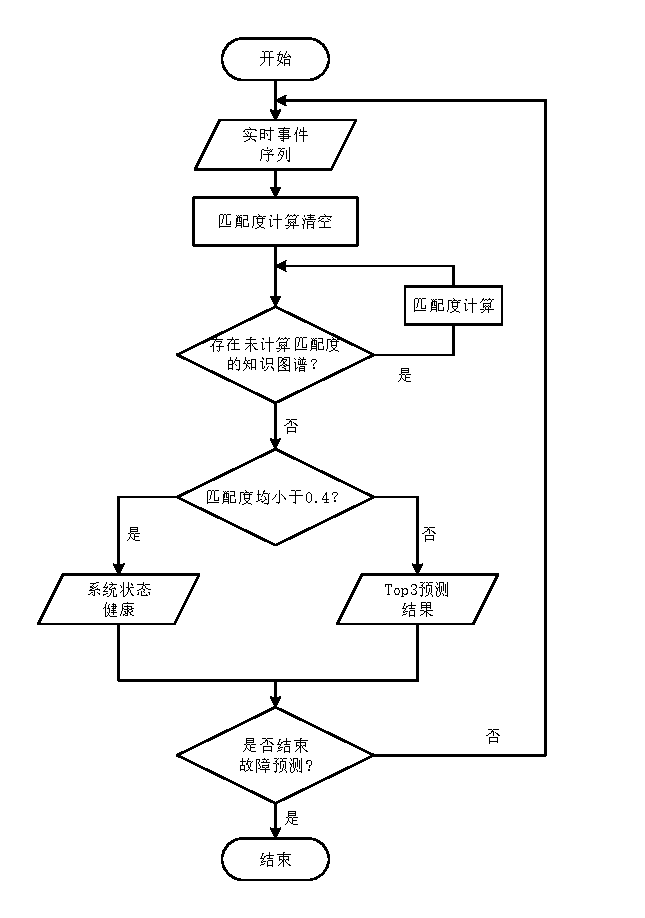
\includegraphics[width=0.6\textwidth]{failure-predict-process.pdf}
    \caption{故障预测程序流程图\label{failure-predict-process}}
\end{figure}

故障预测模块在接受请求后,会运行如图\ref{failure-predict-process}所示的程序。首先,实时事件序列被双向长短期记忆神经网络编码为隐向量。随后,本程序遍历知识库中每种故障类型对应的组件-事件知识图谱,与输入的事件序列计算匹配度。在遍历知识库每张知识图谱计算匹配度的过程中,使用了多线程来加快故障预测速度。当匹配度均小于阈值0.4时,程序会输出集群状态健康的提示;当存在匹配度大于等于0.4的,程序会输出前三的故障预测结果,预测结果为每个匹配的知识图谱对应的故障类型以及其匹配度。本处的阈值0.4是运维人员根据实际运维经验调整设定的。

另外,本模块会对比最匹配的组件-事件知识图谱和实时事件序列,当知识图谱中某条因果关系对应的首尾事件同样在实时事件序列中,就认为该关系为可能的触发关系,合并所有的触发关系即可得到故障触发链。

最后,故障预测模块将预测结果返回到前端。预测结果包含在响应参数中,如以下示例所示。在“result”字段中,“failureType”和“value”依次记录着预测的top3结果及其匹配度值,“nodes”和“links”记录着可能的故障触发链。每一个node都对应着一个具体的事件,所以会有唯一标识、时间戳、位置、事件类型和具体信息5种属性。每个link对应着一条关系,下例中为souce到target的一条cause关系。由于每条属性信息过长,不易于直接展示,所以此处省略了一部分。
\begin{lstlisting}[xleftmargin=6em]
    {
        "status": 200,
        "result": 
        {
            "failureType": [“f3”,“f6”,“f17”,],
            "value": [0.821,0.381,0.217],
            "nodes": [ 
                {
                    "id": "container_cpu_usage...",
                    "time": "1576077480",
                    "location": "container_train...",
                    "event_type": "metric__container...",
                    "detail": "1576077480 pod...",
               }, 
               ... ],
            "links": [ 
                {
                    "source": "k8sevent__BackOff_Warning...",
                    "target": "container_network...",
                    "name": "cause",
                },
                ...]
        }
    }
\end{lstlisting}
% \begin{figure}[htbp]
%     \centering
%     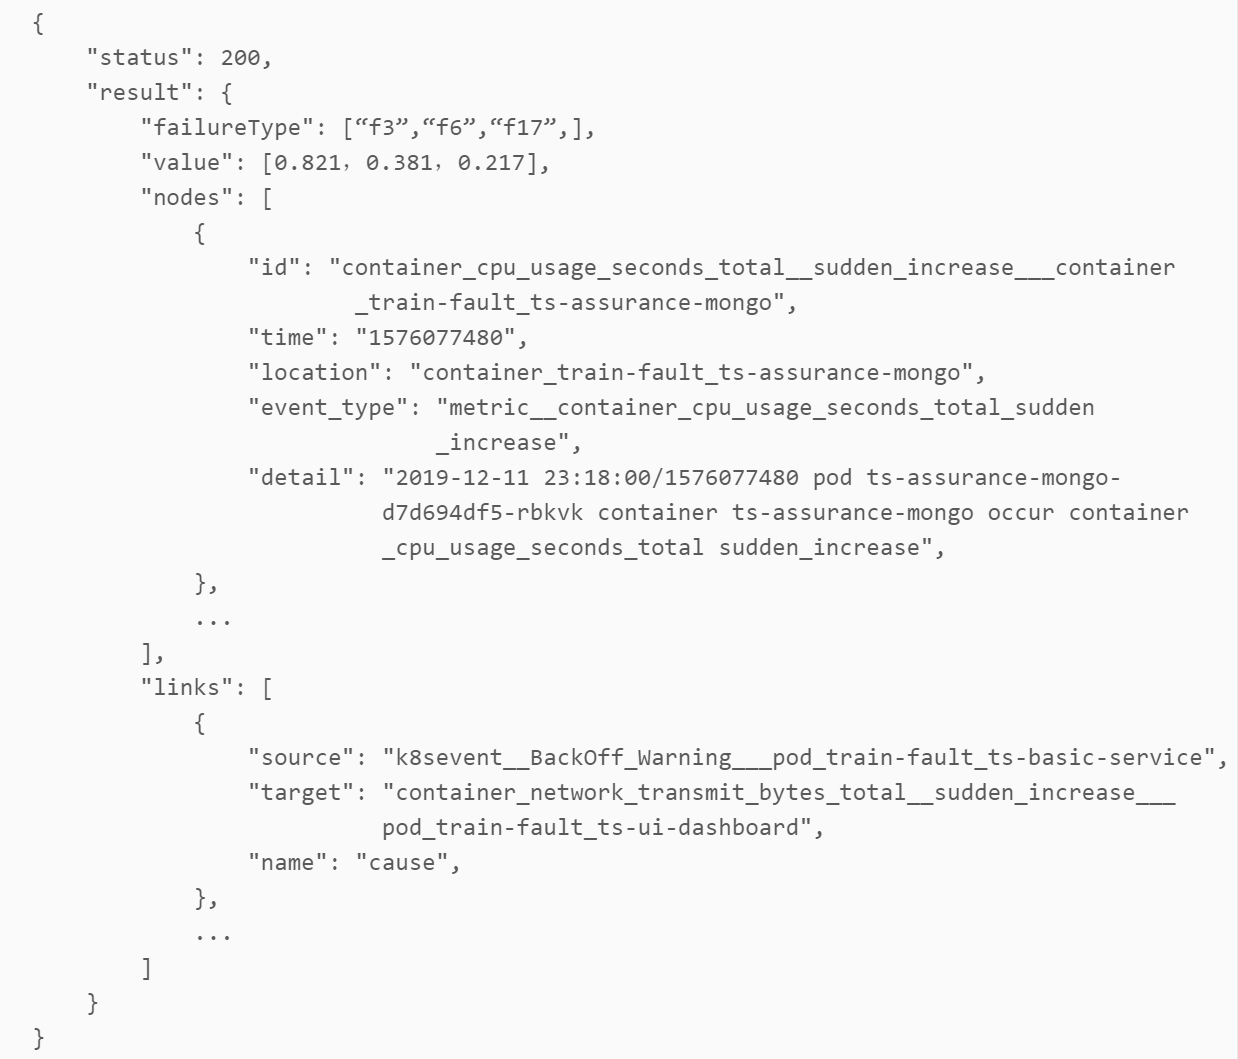
\includegraphics[width=0.8\textwidth]{predict-result.png}
%     \caption{故障预测响应样例\label{predict-result}}
% \end{figure}

\newpage
\section{系统测试}
本章根据章节\ref{need-analysis}中所述的功能性需求和非功能性需求,采用JUnit测试框架对系统进行了测试。本节分为5个小节,分别为系统测试环境、运行状态查询测试、组件事件知识图谱查询及调优测试、实时故障预测测试和系统性能测试。
\subsection{系统测试环境}
本章在进行测试前,记录测试过程所在的环境,包括集群、服务器和各种开发工具版本号,如表\ref{system-test-env}所示。

\begin{table}[htbp]
    \centering
    \caption{系统测试环境}
    \label{system-test-env}
    \begin{tabular}{cc}
    \toprule[1.5pt]
    环境项                        & 环境参数                                                                                                                                        \\ \midrule[1.5pt]
    集群                         & \begin{tabular}[c]{@{}c@{}}集群类型:Kubernetes 托管版\\ 版本:1.12.6-aliyun.1\\ 云服务器个数:30\\ 节点操作系统:CentOS 7.6 64位\\ 节点CPU:8 核\\ 节点内存:16 GiB\end{tabular} \\ \midrule[1pt]
    服务器                        & \begin{tabular}[c]{@{}c@{}}操作系统:Windows 10\\ 处理器:11th Gen Intel(R) Core(TM) i5-11300H\\ 内存:256GB\\ 显存:11GB\\ 硬盘:2TB\end{tabular}            \\ \midrule[1pt]
    Neo4j                      & 版本号4.2.6                                                                                                                                    \\
    Java                       & 版本号1.8.0\_281                                                                                                                               \\
    Python                     & 版本号3.6.8                                                                                                                                    \\
    Kafka                      & 版本号2.2.1                                                                                                                                    \\
    prometheus                 & 版本号2.17.2    \\
    Vue.js                     & 版本号4.5.12    \\
    Spring Boot                & 版本号2.5.0    \\
    \multicolumn{1}{c}{Jaeger} & 版本号1.22.0                                                                                                                                   \\ \bottomrule[1.5pt]
    \end{tabular}
\end{table}

\subsection{运行状态查询测试}
在进行运维工作时,运维人员会有不同的查询需求,本系统实现了常用的查询方式。本小节对实现的各个运行状态查询功能进行了测试,共设计了4条测试用例,分别对应4种查询功能需求,测试结果如表\ref{test-search}所示。测试结果表明各个查询功能均已正确实现,下面展示各个测试用例在前端界面的返回结果。
\newpage
\begin{table}[htbp]
    \centering
    \caption{运行状态查询测试用例}
    \label{test-search}
    \begin{tabular}{cc}
    \toprule[1.5pt]
    内容项  & 描述                                                                                                                                                                                                   \\ \midrule[1.5pt]
    测试目的 & 测试运行状态查询功能                                                                                                                                                                                           \\ \midrule[1pt]
    前置条件 & 测试机联网、系统查询界面可访问                                                                                                                                                                                      \\ \midrule[1pt]
    用例设计 & \multicolumn{1}{l}{\begin{tabular}[c]{@{}l@{}}1.输入查询语句“vpc slb   ecs”,查询符合特定路径类型的所有拓扑,\\点击查询按钮。\\ 2.输入查询语句“vpc id k1aexj”,模糊查询id 包含k1aexj 的vpc 节点,\\点击查询按钮。\\ 3.鼠标悬停在任一组件上方。\\ 4.鼠标左键点击任一组件。\end{tabular}} \\ \midrule[1pt]
    预期结果 & \multicolumn{1}{l}{\begin{tabular}[c]{@{}l@{}}1.返回查询结果,查询结果为符合“vpc slb   ecs”路径类型的所有拓扑。\\ 2.返回查询结果,查询结果是id包含“k1aexj”子序列的vpc节点。\\ 3.组件右上方浮现该组件的属性信息列表。\\ 4.查询页面右侧弹出该组件的所有指标时序数据。\end{tabular}}        \\ \midrule[1pt]
    测试结果 & 4个用例经过测试与预期结果相符合                                                                                                                                                                                     \\ \midrule[1pt]
    状态   & 通过                                                                                                                                                                                                   \\ \bottomrule[1.5pt]
    \end{tabular}
\end{table}
% \hspace*{\fill}
% \begin{itemize}
%     \item 图\ref{search-component-path}显示了搜索符合特定路径类型关系的所有拓扑。如图中所示,在搜索框输入“vpc-slb-ecs”,回车后,下方界面会显示所有由vpc、slb和ecs三种类型组件构成的拓扑结构。
%     \begin{figure}[bhtp]
%         \centering
%         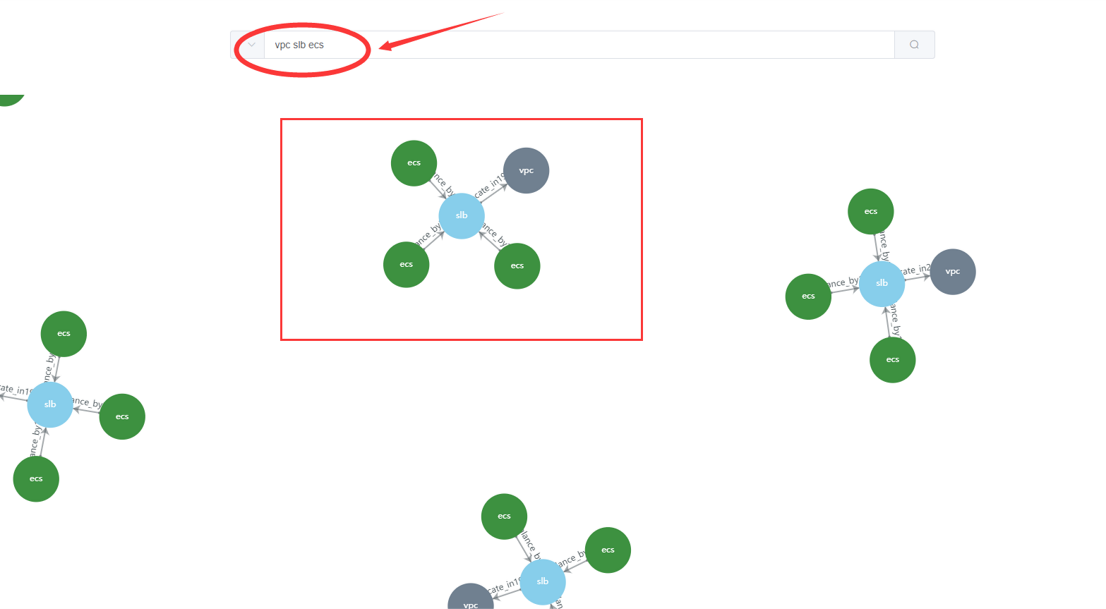
\includegraphics[width=0.7\textwidth,height=0.3\textheight]{search-component-path.png}
%         \caption{搜索指定路径结果\label{search-component-path}}
%     \end{figure}
%     \item 图\ref{search-detail-component}显示了模糊搜索符合某类型某id的组件(如id中包含字段k1aexj的VPC组件)。返回结果除了包含符合条件的组件,还包含该组件的周边组件,便于运维人员查看其上下游拓扑。
%     \begin{figure}[htbp]
%         \centering
%         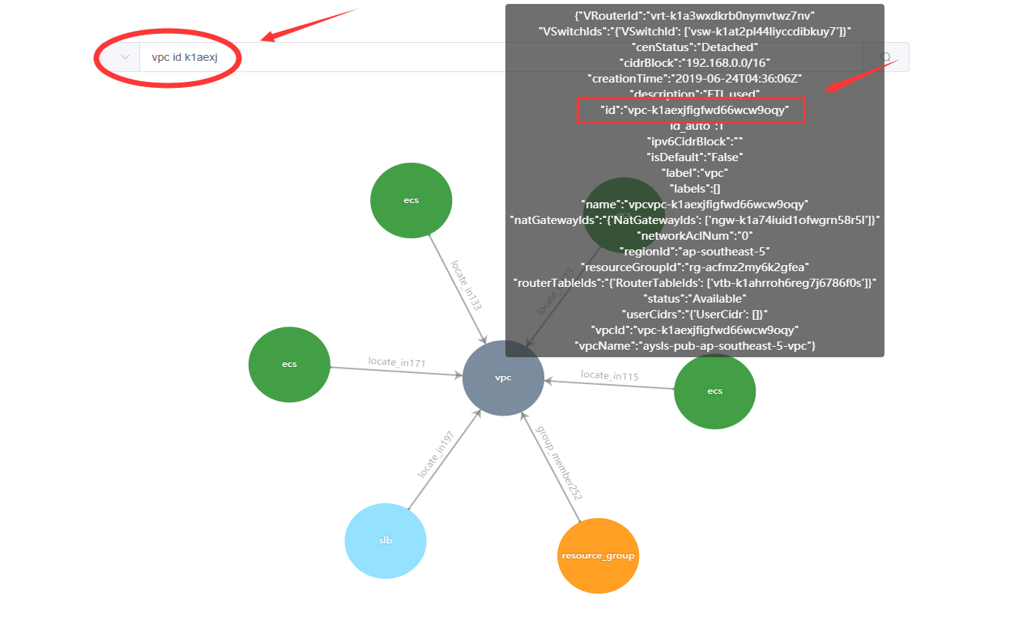
\includegraphics[width=0.9\textwidth]{search-detail-component.png}
%         \caption{模糊搜索结点结果\label{search-detail-component}}
%     \end{figure}
    
%     \item 图\ref{component-detail-info}为组件信息显示界面,在该界面中,组件类型、唯一标识和其间拓扑关系都会被直接展示出来。为了显示组件的所有具体属性信息,将鼠标悬停于组件上,右上方的灰色方框中会浮现该组件的属性信息列表。
%     \begin{figure}[htbp]
%         \centering
%         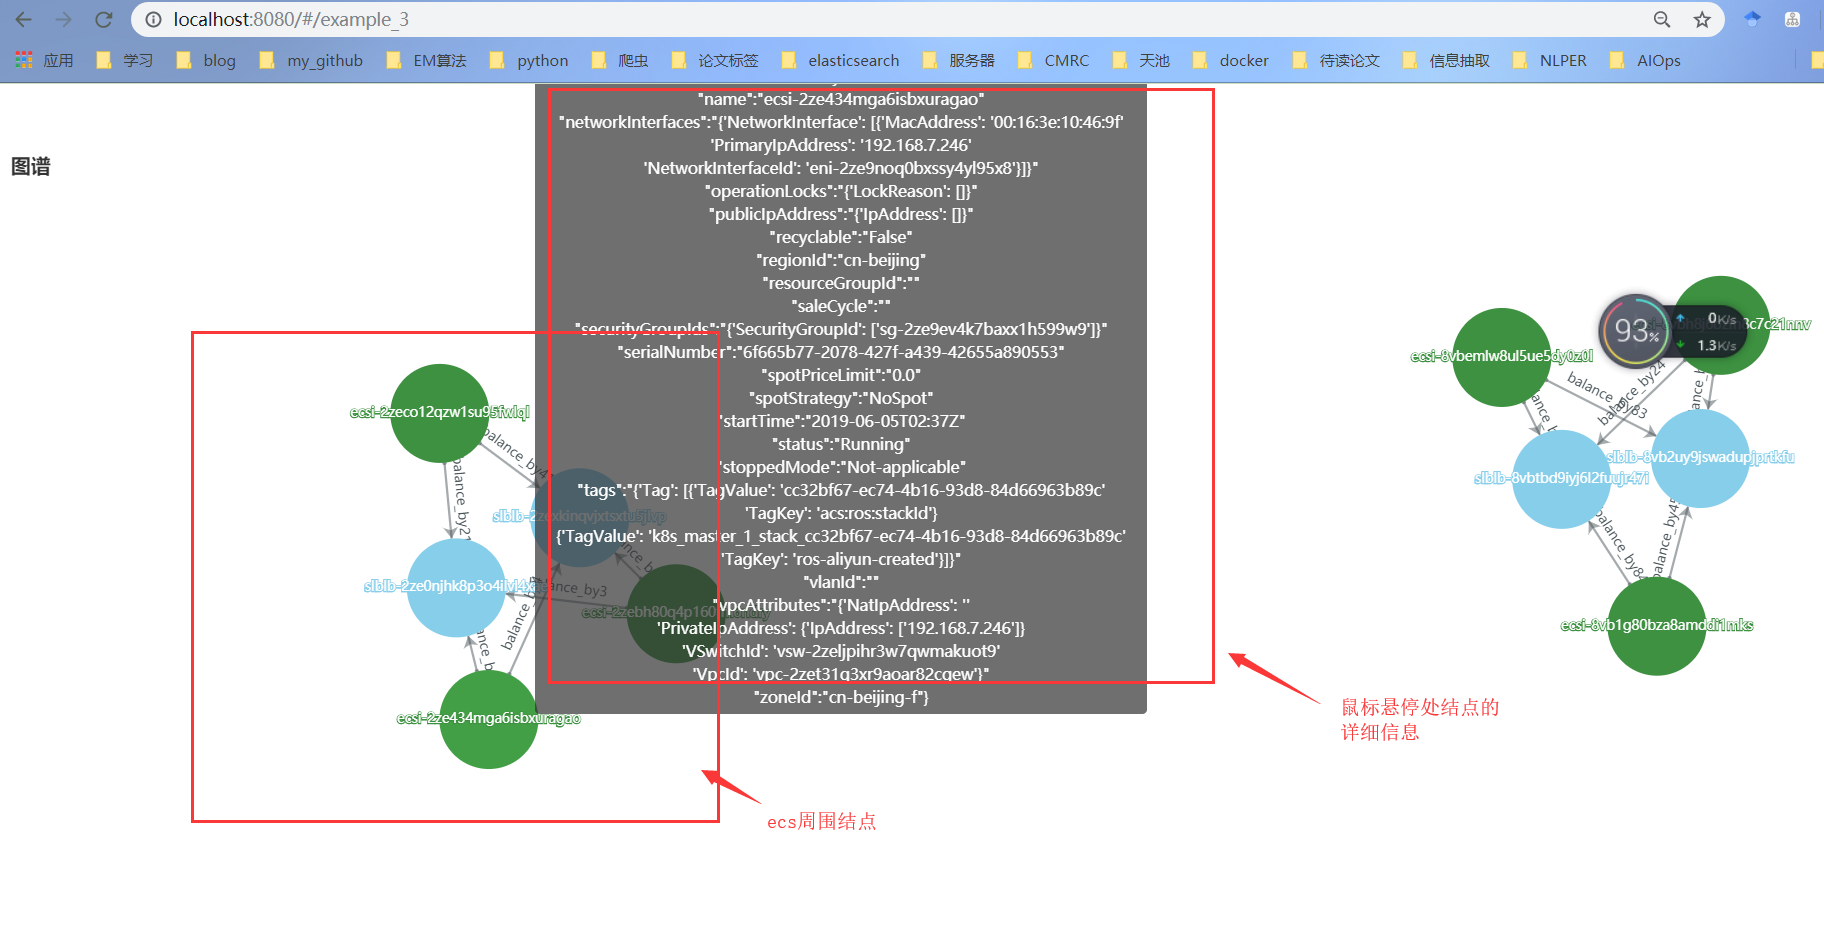
\includegraphics[width=0.9\textwidth]{component-detail-info.png}
%         \caption{查询组件属性信息结果\label{component-detail-info}}
%     \end{figure}
%     \item 对于组件的指标时序数据,可以通过鼠标左键点击组件,右侧抽屉会弹出该组件的各种指标时序数据折线图。如图\ref{search-component-metric-info}所示,在指标时序数据折线图中,上方会显示该组件的唯一标识,中间有该组件多种指标时序数据类型可以选择,下方横坐标可以任意选择展示区间。
%     \begin{figure}[htbp]
%         \centering
%         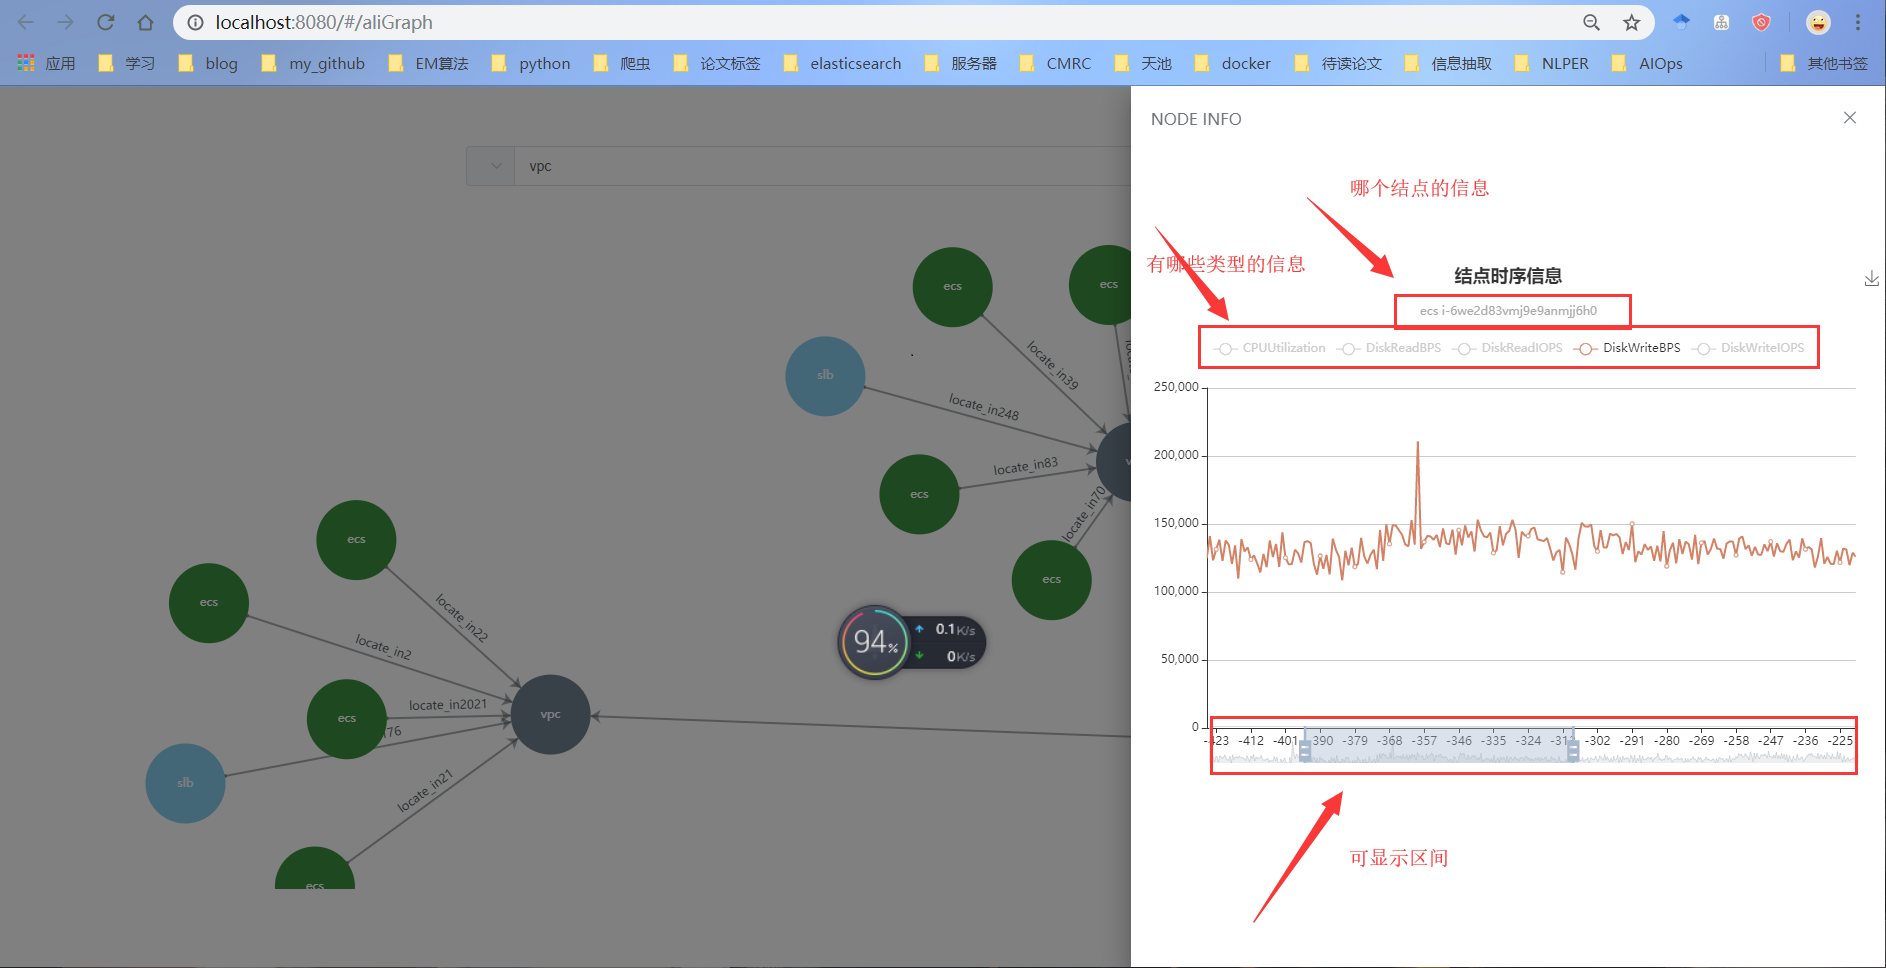
\includegraphics[width=0.8\textwidth]{search-component-metric-info.png}
%         \caption{查询组件指标时序信息结果\label{search-component-metric-info}}
%     \end{figure}
% \end{itemize}

图\ref{search-component-path}显示了搜索符合特定路径类型关系的所有拓扑。如图中所示,在搜索框输入“vpc-slb-ecs”,回车后,下方界面会显示所有由vpc、slb和ecs三种类型组件构成的拓扑结构。
% ,height=0.4\textheight
% \begin{figure}[hbtp]
%     \centering
%     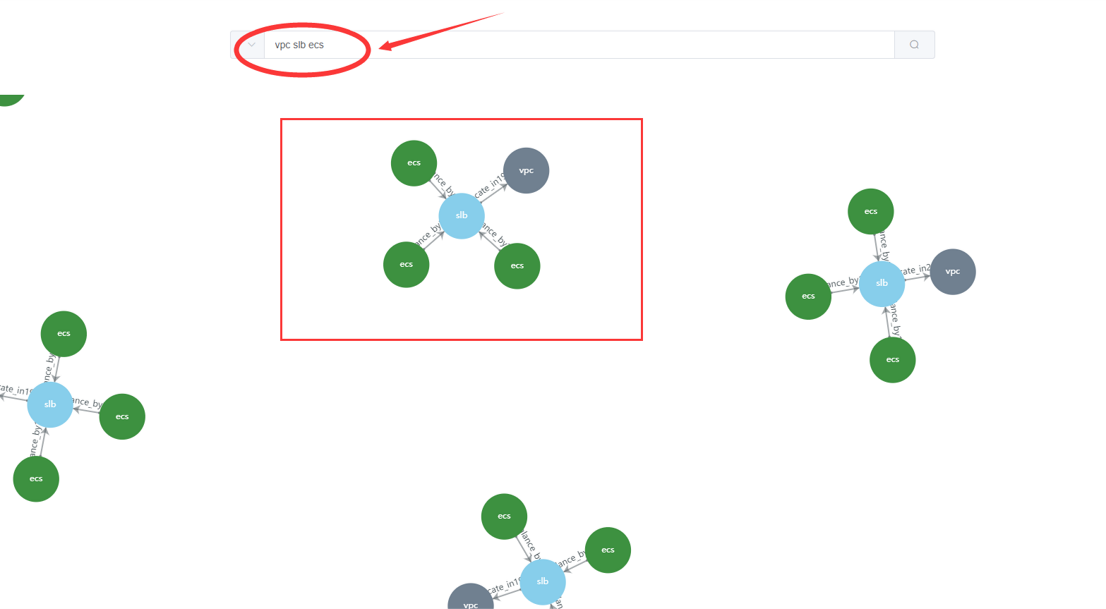
\includegraphics[width=0.75\textwidth,height=0.2425\textheight]{search-component-path.png}
%     \caption{搜索指定路径结果\label{search-component-path}}
% \end{figure}

\begin{figure}[H]
    \center{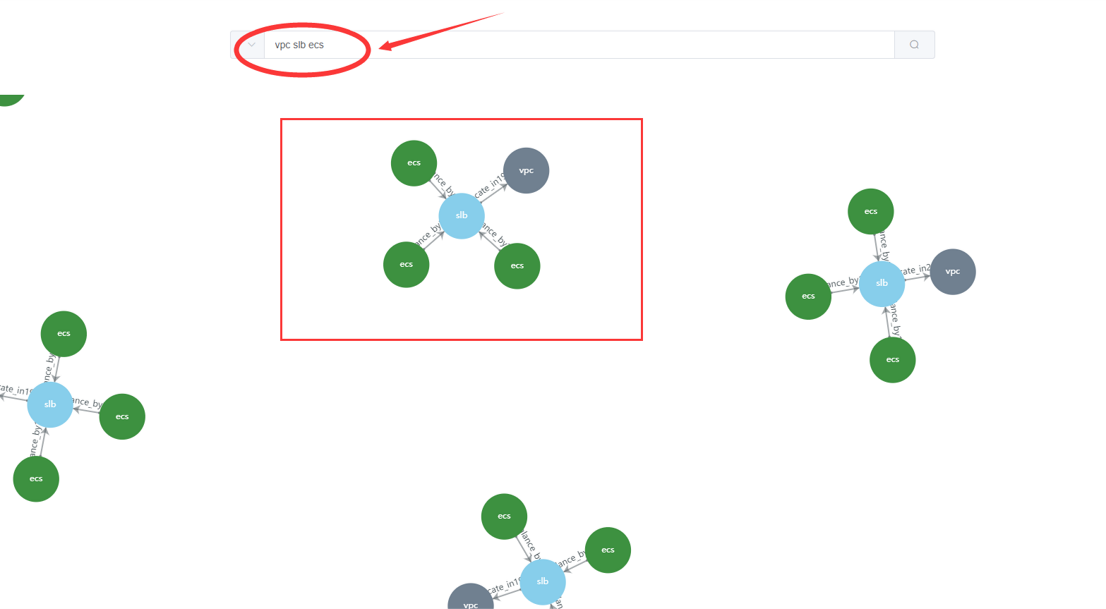
\includegraphics[width=0.95\textwidth]  {search-component-path.png}}
    % 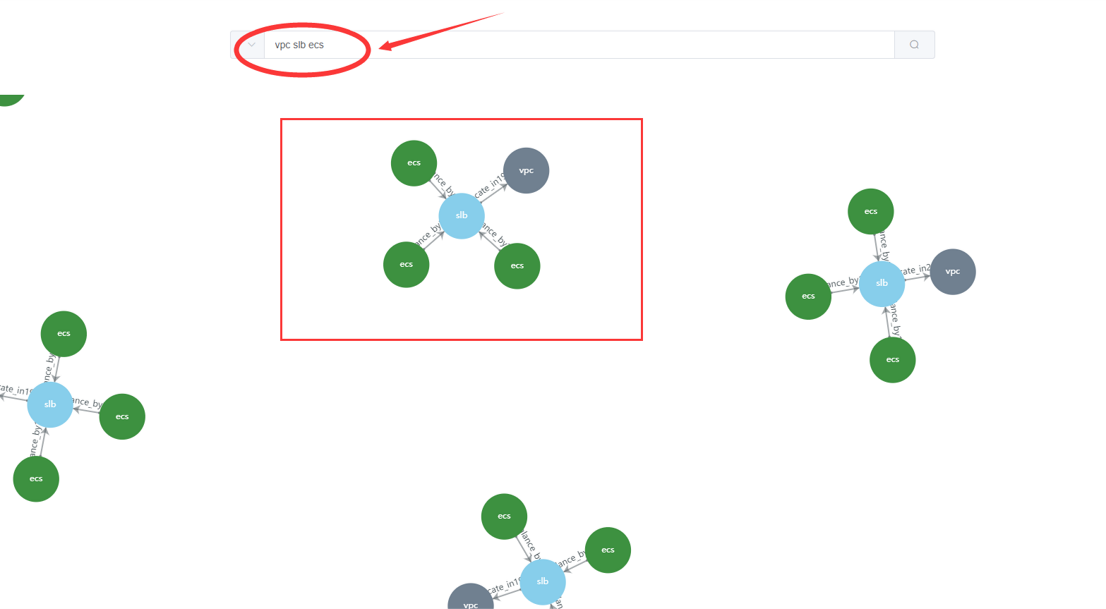
\includegraphics[width=0.4\textwidth]{search-component-path.png}
    \caption{搜索指定路径结果\label{search-component-path}}
\end{figure}
\newpage
图\ref{search-detail-component}显示了模糊搜索符合某类型某id的组件(如id中包含字段k1aexj的VPC组件)。返回结果除了包含符合条件的组件,还包含该组件的周边组件,便于运维人员查看其上下游拓扑。
\begin{figure}[htbp]
    \centering
    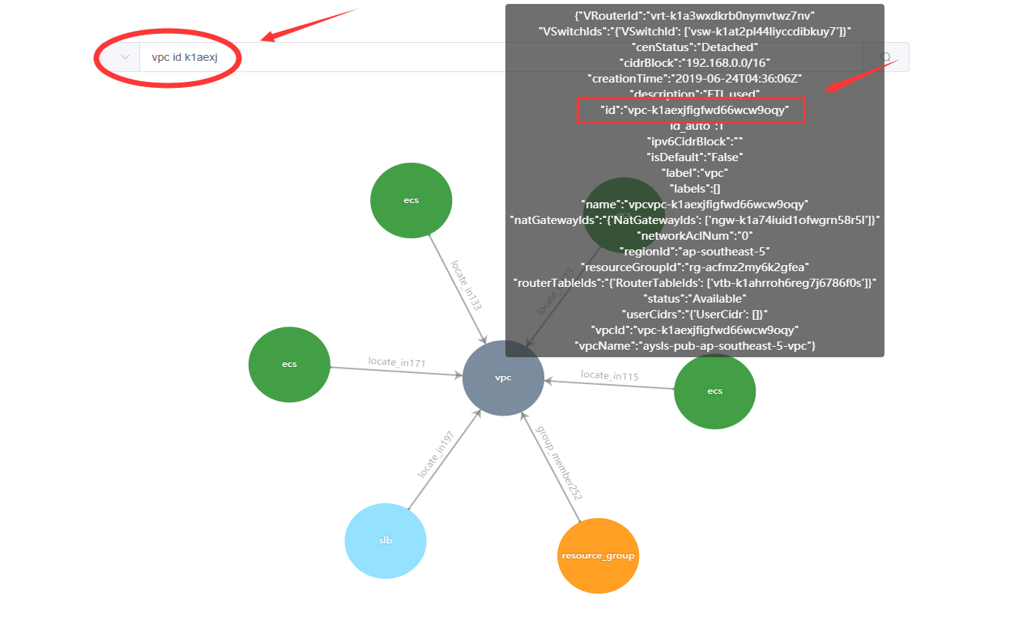
\includegraphics[width=0.9\textwidth]{search-detail-component.png}
    \caption{模糊搜索结点结果\label{search-detail-component}}
\end{figure}

图\ref{component-detail-info}为组件信息显示界面,在该界面中,组件类型、唯一标识和其间拓扑关系都会被直接展示出来。为了显示组件的所有具体属性信息,将鼠标悬停于组件上,右上方的灰色方框中会浮现该组件的属性信息列表。
\begin{figure}[htbp]
    \centering
    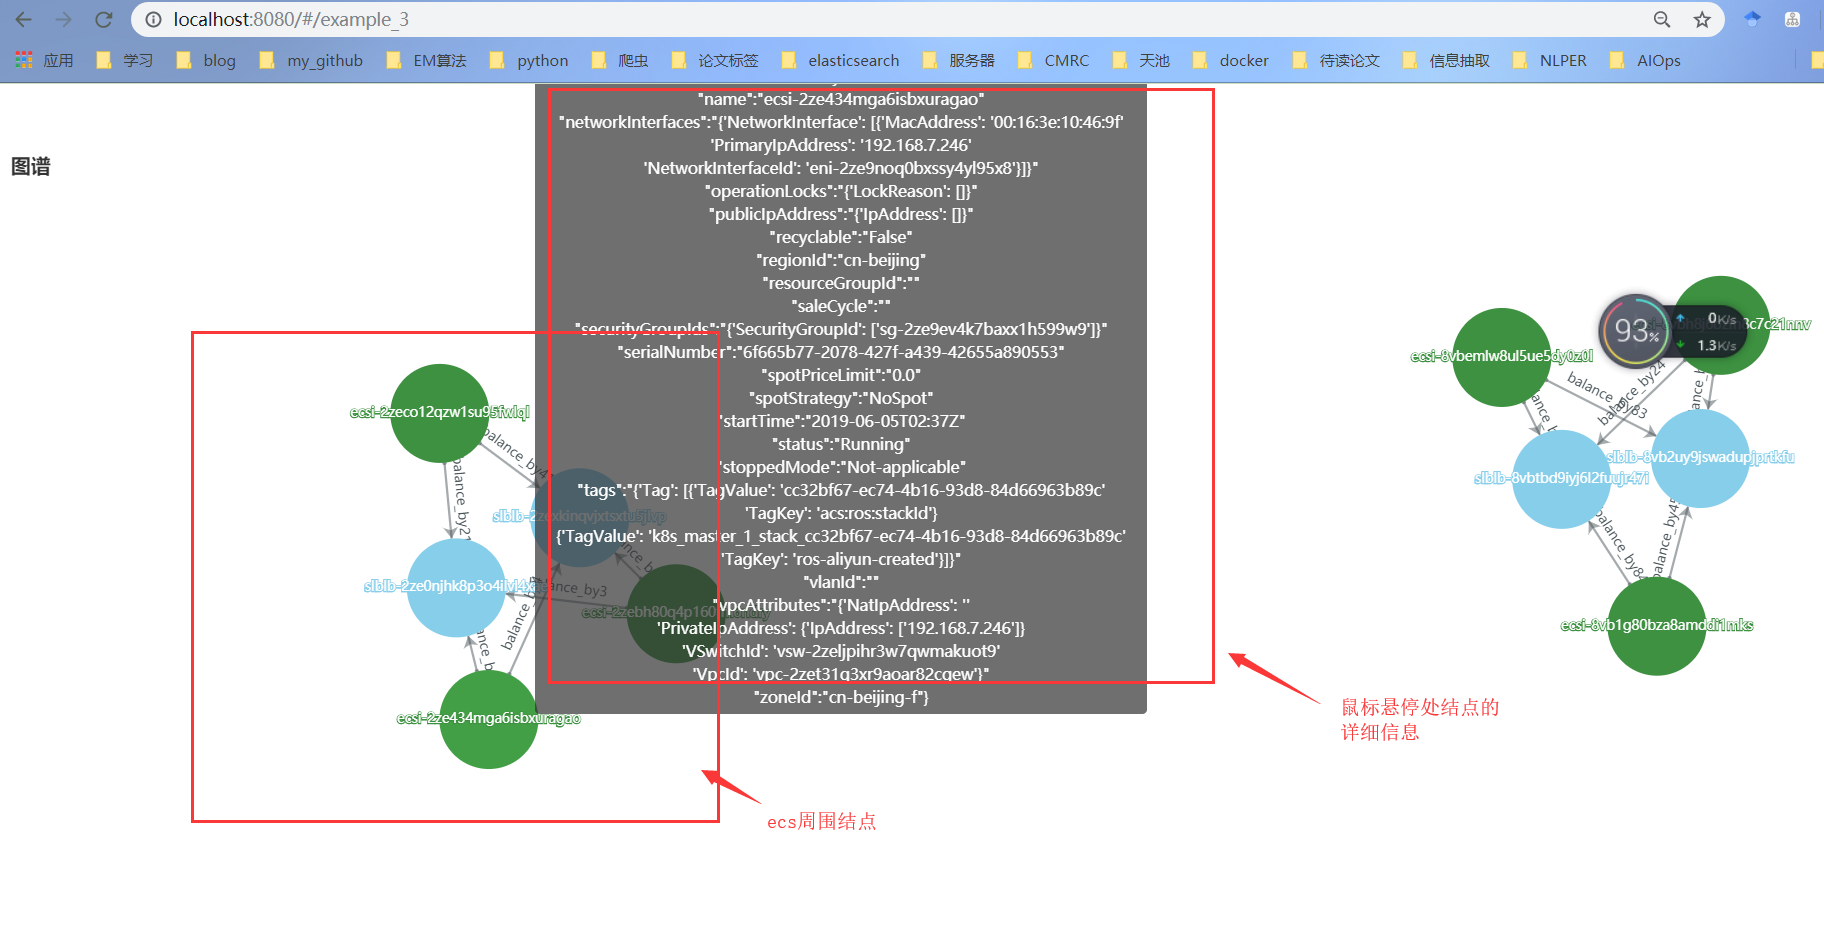
\includegraphics[width=0.9\textwidth]{component-detail-info.png}
    \caption{查询组件属性信息结果\label{component-detail-info}}
\end{figure}

对于组件的指标时序数据,可以通过鼠标左键点击组件,右侧抽屉会弹出该组件的各种指标时序数据折线图。如图\ref{search-component-metric-info}所示,在指标时序数据折线图中,上方会显示该组件的唯一标识,中间有该组件多种指标时序数据类型可以选择,下方横坐标可以任意选择展示区间。
\begin{figure}[htbp]
    \centering
    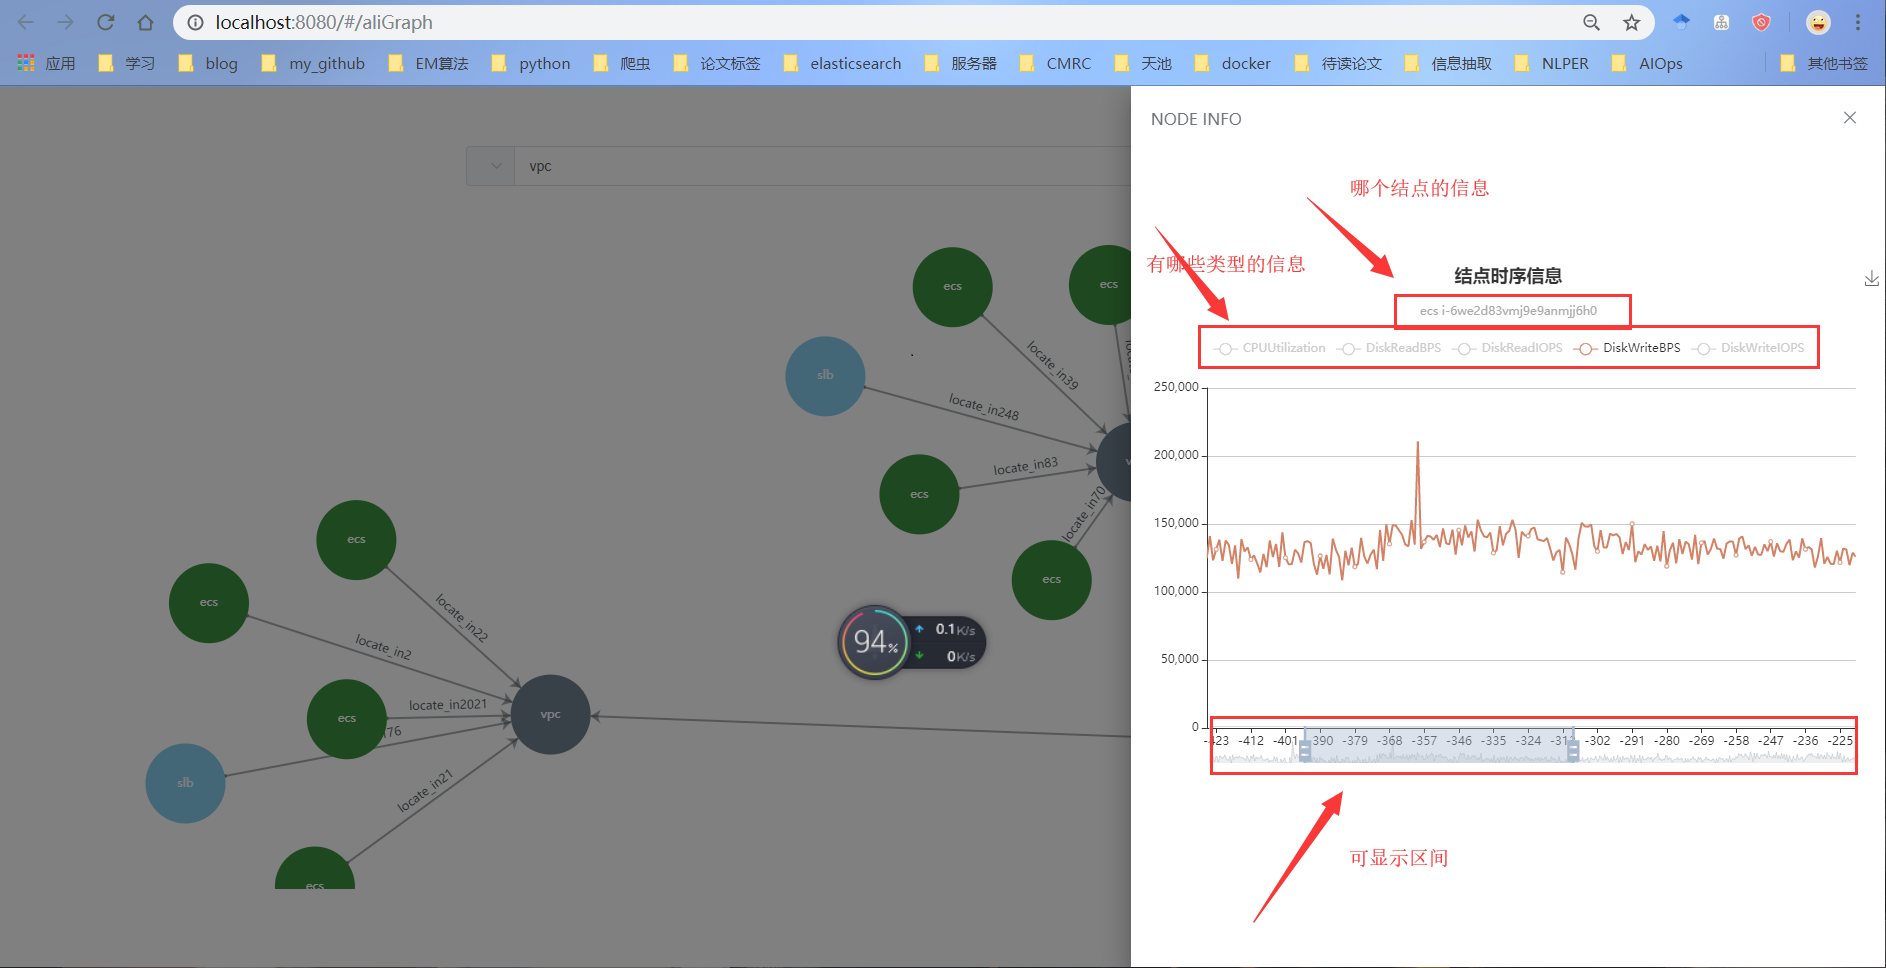
\includegraphics[width=0.9\textwidth]{search-component-metric-info.png}
    \caption{查询组件指标时序信息结果\label{search-component-metric-info}}
\end{figure}

\subsection{组件事件知识图谱查询及调优测试}
本小节对组件-事件知识图谱查询及调优功能进行了测试,共设计了3条测试用例,分别对应查询及调优,测试结果如表\ref{test-graph}所示。
\begin{table}[htbp]
    \centering
    \caption{组件-事件知识图谱查询及调优测试用例}
    \label{test-graph}
    \begin{tabular}{cc}
    \toprule[1.5pt]
    内容项  & 描述                                                                                                                                               \\ \midrule[1.5pt]
    测试目的 & 测试组件-事件知识图谱查询及调优功能                                                                                                                               \\ \midrule[1pt]
    前置条件 & 系统已经存在故障代号为f3的组件-事件知识图谱                                                                                                                              \\ \midrule[1pt]
    用例设计 & \multicolumn{1}{l}{\begin{tabular}[c]{@{}l@{}}1.输入查询语句“f3”,查询故障类型代号为f3的组件-事件\\知识图谱,点击查询按钮。\\ 2.左键任一条边,选择删除,并再次查询“f3”。\\3.选择两个事件结点,单击右键添加一条因果关系,并再次查询“f3”。\end{tabular}}             \\ \midrule[1pt]
    预期结果 & \multicolumn{1}{l}{\begin{tabular}[c]{@{}l@{}}1.返回查询结果,查询结果为故障类型代号为f3的组件-事件知识图谱。\\ 2.返回查询结果,删除的边已经不存在于图中。\\3.返回查询结果,添加因果关系存在于图中。\end{tabular}} \\ \midrule[1pt]
    测试结果 & 3个用例经过测试与预期结果相符合                                                                                                                                 \\ \midrule[1pt]
    状态   & 通过                                                                                                                                               \\ \bottomrule[1.5pt]
    \end{tabular}
\end{table}

图\ref{device-service-event}为查询到的故障代号为f3的组件-事件知识图谱。为了便于查看,整个组件-事件知识图谱使用三层展示:最上层为事件层;中间层为微服务层;下层为部分集群组件层。

\begin{figure}[htbp]
    \centering
    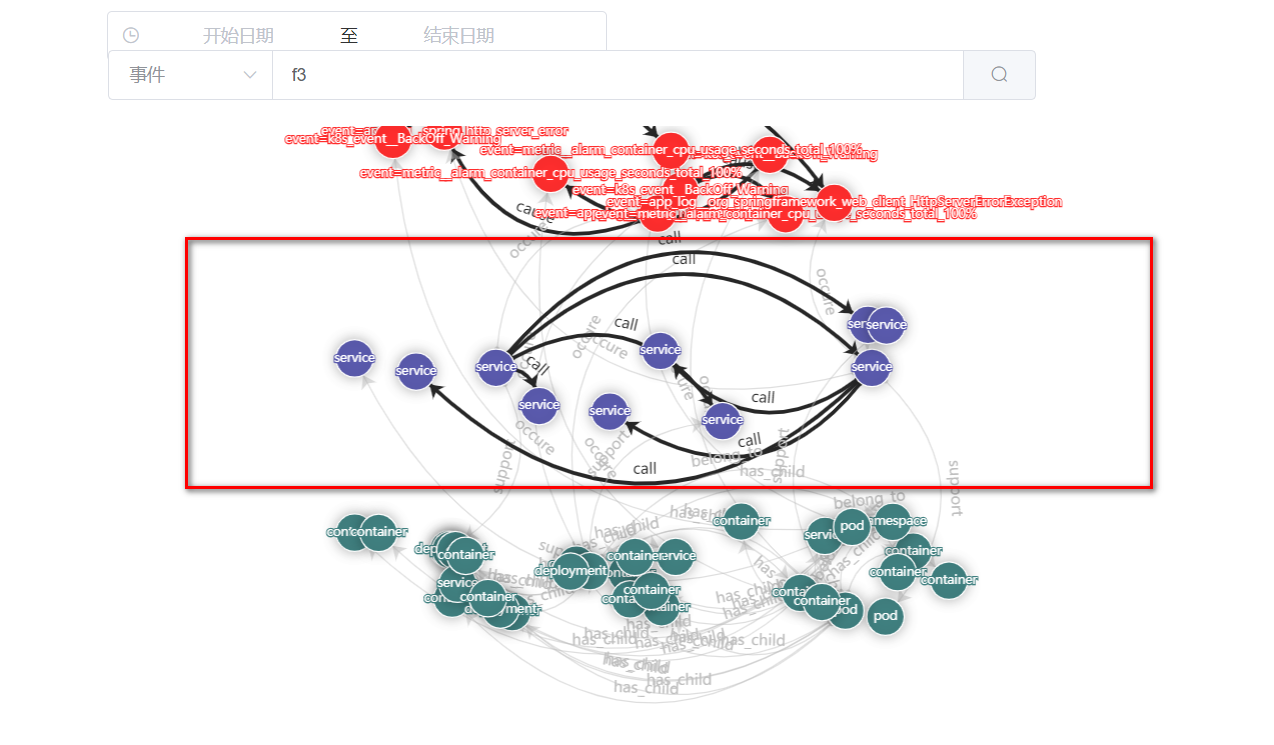
\includegraphics[width=0.85\textwidth]{device-service-event.png}
    \caption{查看f3故障类型的组件-事件知识图谱\label{device-service-event}}
\end{figure}


\subsection{故障预测测试}
本小节对故障预测功能进行了测试,共设计了3条测试用例,测试结果如表\ref{test-predict-failure}所示。
\begin{table}[H]
    \centering
    \caption{故障预测测试用例}
    \label{test-predict-failure}
    \begin{tabular}{cc}
    \toprule[1.5pt]
    内容项  & 描述                                                                                                                                           \\ \midrule[1.5pt]
    测试目的 & 故障预测功能                                                                                                                                       \\ \midrule[1pt]
    前置条件 & 系统存在组件-事件知识图谱,开启了故障检测功能                                                                                                                      \\ \midrule[1pt]
    用例设计 & \multicolumn{1}{l}{\begin{tabular}[c]{@{}l@{}}1.开启故障预测功能,后台注入f3故障的根因异常。\\ 2.关闭故障预测功能,后台注入f3故障的根因异常。\\ 3.开启故障预测功能,后台不注入任何异常。\end{tabular}}   \\ \midrule[1pt]
    预期结果 & \multicolumn{1}{l}{\begin{tabular}[c]{@{}l@{}}1.在故障产生前,页面弹出故障预测top3结果及其对应匹配\\ 度值。\\ 2.故障预测页面未出现任何信息。\\ 3.故障预测页面,一直显示“集群状态健康”。\end{tabular}} \\ \midrule[1pt]
    测试结果 & 3个用例经过测试与预期结果相符合                                                                                                                             \\ \midrule[1pt]
    状态   & 通过                                                                                                                                           \\ \bottomrule[1.5pt]
    \end{tabular}
\end{table}

图\ref{failure-prediction}为实时故障预测界面。在该界面中,实时数据同样以三层结构展示,但发生异常事件的微服务、系统组件节点会显示为红色。当实时数据经过后台故障预测模型判别会出现故障时,右边会弹出故障预测结果窗口,并按照故障类型匹配度由高至低排出前3个最匹配的结果。事件层会显示可能的故障触发链条。
\begin{figure}[htbp]
    \centering
    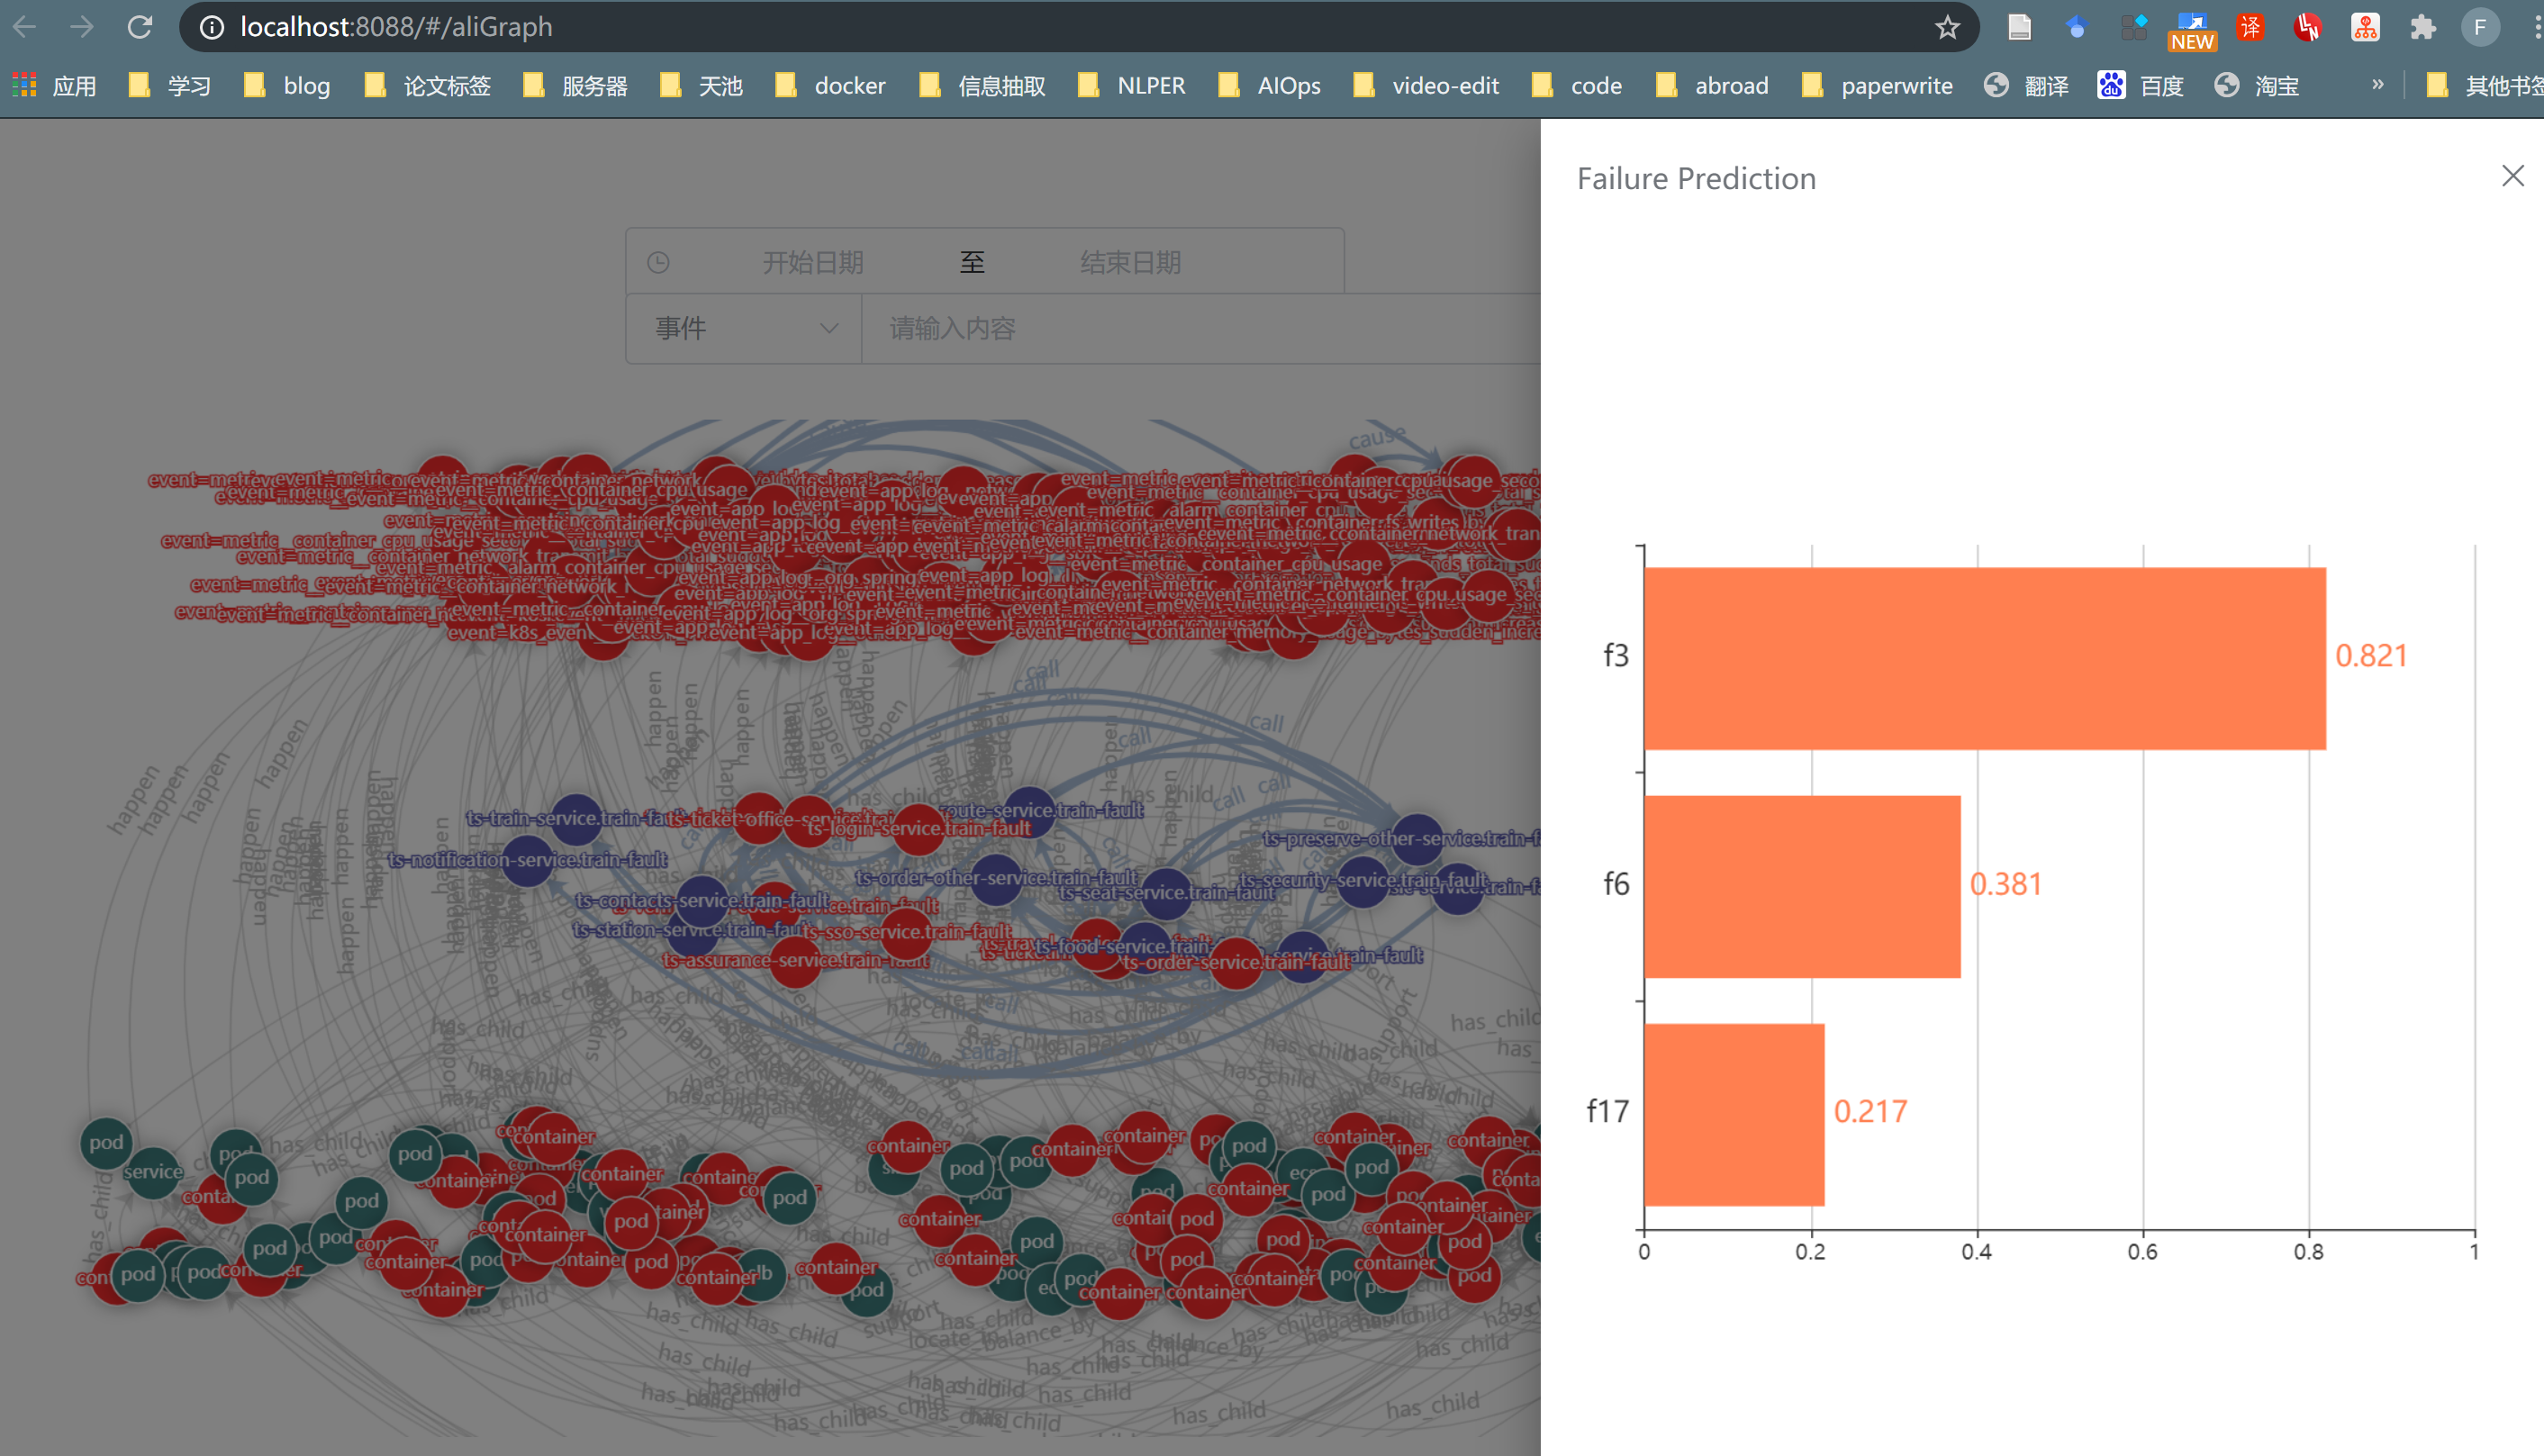
\includegraphics[width=0.8\textwidth]{failure-prediction.png}
    \caption{实时故障预测结果\label{failure-prediction}}
\end{figure}

\subsection{系统性能测试}
本节测试了系统的性能表现,主要包括各个查询功能和故障预测的时间消耗。本节对每一个测试项重复了100次,最终以平均耗时作为测试结果,如表\ref{test-performance}所示。由测试统计结果可见,本系统满足了秒级的系统性能需求。
\begin{table}[htbp]
    \centering
    \caption{系统性能测试}
    \label{test-performance}
    \begin{tabular}{cc}
    \toprule[1.5pt]
    系统性能测试项                                                      & 时间消耗  \\ \midrule[1.5pt]
    查询特定路径类型的拓扑                                                  & 0.65s \\\midrule[1pt]
    模糊查询某个组件                                                     & 0.59s \\\midrule[1pt]
    悬停显示组件信息                                                     & 0.76s \\\midrule[1pt]
    \begin{tabular}[c]{@{}c@{}}左键获取组件\\ 指标时序数据\end{tabular}      & 1.71s \\\midrule[1pt]
    \begin{tabular}[c]{@{}c@{}}搜索某故障类型的\\ 组件-事件知识图谱\end{tabular} & 0.63s \\\midrule[1pt]
    \begin{tabular}[c]{@{}c@{}}注入异常到故障预测\\ 正确并弹出结果\end{tabular}  & 2.38s \\ \bottomrule[1.5pt]
    \end{tabular}
\end{table}

\section{本章小结}
本章分析了IT运维人员在实际工作中的需求,根据第三章、第四章和第五章所提出的各个算法模型,设计了一个基于知识图谱的IT运维辅助系统。随后,本章详细实现了多个功能模块,使得系统可以快速整合多源异构数据、自动沉淀生成组件-事件知识图谱,进行实时故障预测。最后,经过系统测试,证明了本系统可以满足IT运维人员的实际工作需求。

\chapter{总结与展望}
\section{本文工作总结}
本文首先描述了IT运维的研究背景及意义,分析了在实际运维场景中存在的问题:多源异构数据难以整合、运维知识表示不足和故障难以准确预知。随后,本文针对这些问题,对国内外研究现状展开了调研,并分析了已有方案的局限性。本文提出了自动构建组件-事件知识图谱、动态表示组件-事件知识图谱和结合知识图谱进行故障预测的一套算法模型。基于这些算法模型,本文设计并实现了基于知识图谱的IT运维辅助系统。本文完成的工作可分为以下4点:
% 首先,本文设计了事件特征,利用机器学习模型从硬件、软件、日志和指标时序数据中自动地构建组件-事件知识图谱。其次,本文设计了针对组件-事件知识图谱的动态表示学习模型,将实体表示分为语义表示和结构表示,实现了随着实体上下文变化动态地表示实体。最后,本文以上述表示学习模型作为嵌入层,利用双向记忆网络编码事件序列信息,再结合知识图谱进行了故障预测。本文不仅全面地获取并表示了系统多元异构信息,也结合了场景拓扑传播特征、先验知识、实时事件序列进行了表示学习和故障预测。本文完成的工作可分为以下4点:

(1)本文提出了全面整合多源异构数据,自动构建组件-事件知识图谱的方案。在判别事件因果关系时,本文引入了新的事件特征,提升了事件因果关系判别模型的效果。构成的知识图谱包含了高细粒度的多种信息,如软硬组件间关系、指标时序数据和日志数据,解决了多源异构数据难以整合的问题。

(2)本文提出了适配组件-事件知识图谱的动态表示学习模型。该模型将实体表示分为了语义表示和结构表示,语义表示通过实体文本信息获取,结构表示通过Attention-RGCN获取,实现了实体随上下文变化的动态表示,解决了运维知识表示不足的问题。

(3)本文提出了引入知识图谱的故障预测模型。该故障预测模型,利用各类故障对应的知识图谱识别事件序列中的关键信息,把最匹配事件序列的知识图谱作为预测结果,提高了预测结果的细粒度,增强了可解释性,解决了故障难以准确预知的问题。

(4)基于以上工作,本文设计并实现了基于知识图谱的IT运维辅助系统。该系统能够详细展示集群运行状态,并根据实时发生的事件序列和知识图谱预测故障,提醒运维人员及时采取应对措施,满足了实际的IT运维需求。

\section{未来工作展望}
本文深入调研IT运维难点及现有工作不足,提出了结合知识图谱、场景实时特征的基于知识图谱的IT运维辅助方案。但本文所作工作仍有继续优化的空间。

(1)需要在工业界项目上进一步验证效果。目前本系统已在开源的分布式应用train-ticket和sock-shop上取得了良好效果。但工业界应用如淘宝、饿了吗、滴滴等,相较本文使用的两个开源应用,在客户请求量、系统复杂度上都要高出较多量级。因此,本文需要寻求在工业级应用中进一步验证系统性能,并采取相对应的优化措施。

(3)自动生成新的知识图谱,拓展知识库。本文虽然已模拟了常见的十余种故障,但仍难以涵盖实际运行中可能出现的新故障,需要添加业务逻辑自动收集过往未出现的新故障数据并沉淀生成对应的组件-事件知识图谱。
\backmatter
%打印参考文献表
% \chapter{致谢}
恍然间,三年硕士生活已然结束。在东南大学读研的日子里,指导老师、实验室同学和室友均给本人的学习和生活带来了良多帮助,诚心感谢硕士生涯所遇到的诸位良师益友。

科研是一种看似简单而又充满荆棘的认知探索。在科研中,研究生不仅需要有恒心毅力去坚持,还需要有分析问题、提出思路、验证思路的严谨方法论。本人的导师漆桂林教授在科研方面具有丰富的经验与严谨好学的求知态度,引领实验室营造了良好的科研氛围,触动了实验室同学们强烈的科研热情,并常常耐心地指导实验室同学们从事实际的科研工作。本人的硕士毕业论文从开题、模型设计、实验方法到撰写定稿,其间都得到了漆老师的悉心指导。此外,漆老师也经常在生活、职业规划、修身为人方面给予本人诸多教诲,珠玑之言帮助本人形成了正确的价值观与人生观,确立了持续学习、奉献祖国的人生态度。

本人也要感谢实验室的诸位同学。在初入实验室时,花云程博士分享了学校宿舍,使我得以在研究生入学前就开始参与实验室的科研项目。在工程项目中,李林、罗安源、吴畏、李震等同学帮助我补全科研知识、提高工程能力,一起顺利完成项目结题。实验室的师兄也经常提供科研与生活方面的建议,每当科研受阻、思路难寻、或生活受挫时,吴天星、花云程、吴桐桐、毕胜诸位博士都会提出宝贵的意见。在日常起居方面,本人真心感谢蒋志强、李同哲、丛宏宇、李蒙、支伯川和傅汉霖同学,不仅共同维护了良好的宿舍环境,也经常互相督促学习共同进步。

最后,本人真诚感谢父母、妹妹与弟弟,家人不仅给予了求学所需的物质基础,也在生活受挫时给予了我安慰与鼓励。幸福的家庭氛围给予了本人面对生活、工作和求学的本源信心与动力。

























% 时光如同奔流的长河,一去不回来不及道别。转眼间三年飘然离去,回忆中刚进实验室时,应是我一生中最浪漫的瞬间。

% 科研是一种难以捉摸又让人兴奋致死的东西。平凡的生命会因科研而火热,也会因它错过周六的约会。往后的日子里余波荡漾,再看你一眼,我就头也不回的走了,我的蒙娜丽莎,我只有真心而已。
\thesisbib

\appendix


% \resume{作者攻读硕士学位期间的研究成果}
% \begin{flushleft}
%     {\bfseries \large 发表的论文}\\ \relax
%     [1] 智能运维中事件知识图谱的构建与事件表示学习[J].东南大学计算机科学与工程学院学术论坛,2021.(第一作者)\\
% \end{flushleft}

\end{sloppypar}
\end{document}
% 在线表格生成工具https://json.im/tableConvert/   https://www.tablesgenerator.com/latex_tables  https://www.tablesgenerator.com/#
% 知识规则抽取工具 https://zhuanlan.zhihu.com/p/353043426